\documentclass{article}
\usepackage{lmodern}
\usepackage[francais]{babel}
\usepackage[utf8]{inputenc}
\usepackage{graphicx}
\usepackage{shortvrb}
\usepackage{amssymb}
\usepackage{amsmath}
\usepackage{listings}
\usepackage{mathtools}
\usepackage{soul}
\usepackage{color}
\usepackage{fancyhdr}
\usepackage{verbatim}
\usepackage{geometry}
\usepackage{tikz}
\geometry{hmargin=2.5cm,vmargin=2.5cm}
\pagestyle{fancy}
%\renewcommand{\footrulewidth}{0.4pt}
\renewcommand{\headrulewidth}{0.4pt}
\lhead{Introduction à la théorie des ondelettes}
\rhead{Xavier Friederich et Gaétan Bahl}

\title{TIPE: Introduction à la théorie des ondelettes}
\author{Xavier Friederich et Gaétan Bahl}

\begin{document}
\maketitle
\tableofcontents
\listoffigures
\MakeShortVerb{@}
\clearpage

\newcommand{\fonction}[5]{\begin{array}{l|rcl}
#1: & #2 & \longrightarrow & #3 \\
    & #4 & \longmapsto & #5 \end{array}}



\section{L'analyse de Fourier, outil certes efficace mais insuffisant}

Les séries de Fourier (pour les signaux périodiques) et la transformée de Fourier (pour un signal quelconque) ont longtemps été les outils essentiels de l'analyse harmonique. \\
Le but de cette première partie est de présenter brièvement l'analyse de Fourier et de montrer ses limites.

\subsection{Le cas des signaux périodiques : l'utilisation des séries de Fourier}

Considérons $f$ fonction $2\pi$-périodique de classe $\mathcal{C}^{1}$ par morceaux. \\
Notons $S_{p}(f)$ la p-ième somme partielle de Fourier de $f$, ou p-ième somme partielle de la série de Fourier de $f$. \\
On a : $$ S_{p}(f)=\sum_{n=-p}^{p}c_{n}(f)e^{int} $$ en notation exponentielle ou bien $$ S_{p}(f)=\displaystyle\frac{a_{0}}{2}+\sum_{n=1}^{p}\left(a_{n}(f)\cos(nt)+b_{n}(f)\sin(nt)\right)$$ en notation trigonométrique ; \\
les $a_n$ et $b_n$ étant donnés par les relations 
$$ a_n=\displaystyle\frac{1}{\pi}\int_{0}^{2\pi}f(t)\cos(nt)\mathrm{d}t$$
$$ b_n=\displaystyle\frac{1}{\pi}\int_{0}^{2\pi}f(t)\sin(nt)\mathrm{d}t$$
\\
Le cours de mathématiques (plus particulièrement le théorème de Dirichlet) nous donne alors le résultat bien connu suivant, avec les hypothèses sur $f$ données plus haut : \\
\\
$f$ est somme de sa série de Fourier, ce qui se réécrit de la façon suivante :
$$\forall t\in\mathbb{R}, f(t)=\displaystyle\frac{a_{0}}{2}+\sum_{-\infty}^{+\infty}\left(a_{n}(f)\cos(nt)+b_{n}(f)\sin(nt)\right)$$
\\
On peut ainsi très facilement décomposer un signal périodique en une somme infinie de sinusoïdes. 

\pagebreak

\begin{figure}[!h]
\centering
<<<<<<< HEAD
\includegraphics[scale=0.2]{sinusoides.png}
=======
\includegraphics[scale=0.2]{images/sinusoides.png}
>>>>>>> d5245ec323332736ffd68589bb833e4bf5a5f8bb
\caption{Illustration du théorème de Fourier pour les signaux périodiques}
\end{figure}
Le signal "carré" en noir est la somme de toutes les sinusoïdes représentées, la sinusoïde rouge d'amplitude majeure étant appelée $\mathit{fondamentale}$ et les autres sinusoïdes étant les $\mathit{harmoniques}$. \\

 Bien évidemment, la plupart des signaux que l'on peut rencontrer sont non-périodiques et il est impossible d'obtenir une décomposition analogue à celle décrite ci-dessus. Dans le cas général et dans la limite de la possibilité de le faire, on effectue une transformation de Fourier.

\subsection{L'utilisation de la transformée de Fourier}

Il est nécessaire dans le cas plus général de fonctions/signaux non nécessairement périodiques de passer d'une écriture discrète en uneécriture en somme continue.
\\
Le cadre le plus naturel pour définir les transformations de Fourier est celui des fonctions $f$ intégrables\footnote{continues par morceaux et telles que $ \exists M \in \mathbb{R},\forall I\subset\mathbb{R}, \left|\int_{I}f(x)\right|\leq M$}. 
\\
On note alors traditionnellement $\mathcal{L}^{1}(\mathbb{R})$ l'ensemble des fonctions intégrables sur $\mathbb{R}$ et  $\mathcal{L}^{2}(\mathbb{R})$ l'ensemble des fonctions de carré intégrable sur $\mathbb{R}$.


\subsubsection{Définition de la transformation de Fourier}
 
On appelle transformation de Fourier l'application notée $\mathcal{F}$ qui, à toute fonction $f$ de  $\mathcal{L}^{1}(\mathbb{R})$, associe la fonction $\hat{f}$ telle que $\forall \omega \in \mathbb{R}$,$ \hat{f}(\omega)=\displaystyle{\frac{1}{\sqrt{2\pi}}\int_{-\infty}^{\infty}f(t)e^{-i\omega t}\:\mathrm{d}t}$
\\
$\hat{f}$ est appelée transformée de Fourier de $f$.
\\ \\
Notons toutefois que l'on peut donner plusieurs versions de définitions : nous avons ici choisi la définition plus "physicienne", car on y voit directement les paramètres de temps ($t$) en $s$ et de pulsation ($\omega$) en  $rad.s^{-1}$.
\\ \\
Notons aussi qu'il est possible de définir la transformée de Fourier pour des fonctions qui ne sont pas forcément dans $\mathcal{L}^{1}(\mathbb{R})$.
\\
\subsubsection{Propriétés de la transformation de Fourier} 
\begin{itemize}
\item $\mathcal{F}$ est clairement linéaire. \\
\item On peut montrer que $\mathcal{F}$ conserve la parité. \\
\item Propriété de translation : \\ Soit $a \in \mathbb{R}$ et $f\in \mathcal{L}^{1}(\mathbb{R})$ de la variable $t$. En effectuant le changement de variable $u=t-a$, on obtient la transformée de Fourier de la fonction d'expression $f(t-a)$. En effet : 
$$ \mathcal{F}[f(t-a)]=\displaystyle\int_{-\infty}^{\infty}f(t-a)e^{-i\omega t}\:\mathrm{d}t=\displaystyle e^{-i\omega a}\int_{-\infty}^{\infty}f(u)e^{-i \omega u}\:\mathrm{d}u=\displaystyle e^{-i\omega a}.\hat{f}(\omega) $$

\end{itemize}
 

\subsubsection{Transformée inverse}

On utilise les mêmes notations que précédemment.
Si $\hat{f}$ est elle-même une fonction intégrable, la formule dite de transformation de Fourier inverse, opération notée $\mathcal{F}^{-1}$ , et appliquée à $\hat{f}$, permet (sous conditions appropriéees) de retrouver $f$ :
$$ f(t)=\displaystyle{\frac{1}{\sqrt{2\pi}}\int_{-\infty}^{\infty}\hat{f}(\omega)e^{i\omega t}\:\mathrm{d}\omega}$$

Cette formule peut se démontrer facilement à partir de la formule sommatoire de Poisson.

\subsubsection{Ce qu'apporte la transformée de Fourier d'un signal}
Dans le cas général, la transformation de Fourier d'une fonction produit comme transformée une fonction $\hat{f}$ à valeurs complexes. Ainsi, on peut obtenir deux informations de cette transformée :

Le spectre d'amplitude : il s'agit du tracé du module de $\hat{f}(\omega)$ en fonction de la pulsation $\omega$.

Le spectre de phase :  il s'agit du tracé de l'argument de $\hat{f}(\omega)$ en fonction de la pulsation $\omega$.

Notons que l'on rencontre très souvent en traitement du signal les spectres en fréquence ; on passe de la pulsation $\omega$ à la fréquence par la relation de proportionnalité suivante : $f=\displaystyle \frac{1}{2\pi}\omega $.

On remarquera, comme le montre la figure ci-dessous, que le spectre d'amplitude d'un signal périodique est formé de traits verticaux.
\begin{figure}[!h]
\centering
<<<<<<< HEAD
\includegraphics[scale=0.4]{spectre.jpg}
=======
\includegraphics[scale=0.4]{images/spectre.jpg}
>>>>>>> d5245ec323332736ffd68589bb833e4bf5a5f8bb
\caption{Spectre de Fourier en fréquence d'un signal périodique}
\end{figure}

\subsubsection{Exemples de transformée de Fourier}

Facilement, on peut montrer que la transformée de Fourier d'une gaussienne\footnote{une fonction en $e^{\frac{-x^2}{2}}$.} est une gaussienne.
\begin{figure}[!h]
\centering
<<<<<<< HEAD
\includegraphics[scale=0.3]{gaussienne.png}
=======
\includegraphics[scale=0.3]{images/gaussienne.png}
>>>>>>> d5245ec323332736ffd68589bb833e4bf5a5f8bb
\caption{Allure d'une gaussienne}
\end{figure} \\ \\

Si on note $\Pi$ la fonction porte définie par 
$\forall t\in \left[-\frac{1}{2},\frac{1}{2} \right],\Pi(t)=1$ et $\forall t\in \mathbb{R} \backslash \left[-\frac{1}{2},\frac{1}{2} \right],\Pi(t)=0$, on obtient directement par intégration de l'exponentielle complexe et en tenant compte de la relation $\sin x = \displaystyle\frac{e^{ix}-e^{-ix}}{2i}$,
$\mathcal{F}(\Pi)(\omega) = \mathrm{sinc}(\frac{\omega}{2})$.  \footnote{la fonction sinc (sinus cardinal) est au premier sens mathématique la fonction définie sur $\mathbb{R}$* par sinc$(x)=\frac{\sin x}{x}$.} \\ La fonction étant réelle, son spectre de phase correspond à la fonction nulle et son spectre d'amplitude est le suivant : 
\begin{figure}[!h]
\centering
<<<<<<< HEAD
\includegraphics[scale=0.5]{sinc.jpg}
=======
\includegraphics[scale=0.5]{images/sinc.jpg}
>>>>>>> d5245ec323332736ffd68589bb833e4bf5a5f8bb
\caption{Spectre d'amplitude de la fonction $\Pi$}
\end{figure}


\subsubsection{Application de la transformation de Fourier}
En physique, la transformation de Fourier permet de déterminer le spectre d'un signal. 

En traitement d'images, on effectue des transformations de Fourier à deux dimensions : si $f$ est une fonction de $\mathbb{R}^2$ , sa transformée de Fourier est définie par : $$\hat{f}(u,v)=\int_{-\infty}^{\infty}\int_{-\infty}^{\infty}f(x,y).e^{-i(ux+vy)}\:\mathrm{d}x\:\mathrm{d}y$$
\\
On comprendra que la très grande majorité des signaux sont numériques et que les définitions mathématiques données jusqu'à présent ne sont pas adaptées au domaine du discret.

\subsection{Transformée de Fourier Discrète ou TFD et limites}

Bien évidemment, la transformée de Fourier telle qu'elle est utilisée dans un ordinateur (transformée de Fourier discrète (TFD)) possède une définition numérique différente de la définition mathématique donnée plus haut. 

\subsubsection{Définition}

Nous nous placerons dans le cas complexe (le cas réel en découle) sur un intervalle de temps fini correspondant à $N$ échantillons. Quand $N$ tend vers l'infini, on peut penser que l'on s'approche du cas continu mais il faut garder à l'esprit que la TFD suppose que le signal est périodique de période $N$.
\\ \\
Nous proposons la définition de la TFD d'un point de vue de l'algèbre linéaire, qui semble plus schématique :
\\
On définit ainsi la TFD comme un endomorphisme de $\mathbb{C}^N$ ayant pour matrice dans la base canonique de $\mathbb{C}^N$ la matrice S de terme général $s_{j,k}=\displaystyle{\frac{1}{N}e^{-2i\pi \frac{jk}{N}}}$, où $j,k\in \left\{0,1,...,N-1\right\}$. 
\\ \\
La TFD s'applique ainsi à des suites de longueur N (ou de période N) et on peut d'ailleurs remarquer que la TFD est périodique de période N.
\\ \\
On obtient ainsi, en l'appliquant à un vecteur $f=(f_0,...,f_{N-1})$ de $\mathbb{C}^N$ de matrice $F\in \mathcal{M}_{N,1}(\mathbb{C})$, le vecteur $g=(g_0,...,g_{N-1})$ de matrice $G=S$$\times$ $F$.
\\ On a clairement de la définition et du produit matriciel : 
$$\forall j\in \left\{0,1,...,N-1\right\}, g_j=\displaystyle\sum_{k=0}^{N-1}\displaystyle{\frac{1}{N}e^{-2i\pi \frac{jk}{N}}}f_k$$

En notant $W$ l'inverse de la racine $N$-ième de l'unité\footnote{$W=e^{\displaystyle-\frac{2i\pi}{N}}$}, il vient bien sûr : 
\begin{center}
\begin{equation}
$$$\forall j\in \left\{0,1,...,N-1\right\}, g_j=\displaystyle\sum_{k=0}^{N-1}W^{kj}f_k$$$
\end{equation}
\end{center}

\subsubsection{Des applications de la TFD}
La TFD a plusieurs applications, parmi lesquelles :  \\
\begin{enumerate}
\item L'analyse spectrale des signaux. \\ Il est intéressant pour un électronicien de mesurer par exemple la largeur de la bande de fréquence occupée par la transmission d'un signal, ceci grâce à une analyse spectrale. \\
\item La compression de données. \\  On applique sur les signaux la TFD pour réduire leur complexité. La suite des coefficients obtenus (en appliquant la formule ($1$)) est alors quantifiée avec des pas de quantification plus élevés pour les hautes fréquences, considérées comme négligeables pour la perception humaine. Le gain en compression vient de la réduction de précision de ces coefficients (voire leur suppression totale) : cela nécessite de ce fait moins de bits pour le codage.
\item La multiplication des grands nombres. \\ Certains des algorithmes les plus rapides (type FFT) pour la multiplication de grands nombres entiers sont fondés sur la TFD. 

\end{enumerate}

 Néanmoins, toutes ces applications nécessitent l'existence d'un algorithme rapide de calcul de la TFD et de son inverse. Les multiplications dans les cas où $N$ est petit sont "triviales", mais quand $N$ devient grand il est en effet indispensable d'utiliser un tel algorithme permettant de diminuer le nombre de multiplications. 


\subsubsection{Des limites à la Transformée de Fourier Discrète}
La TFD présente des limites considérables.
\\
On ne peut pas analyser un morceau de musique avec une TFD simple. En effet, on perdrait l'information temporelle.
Prenons par exemple deux signaux semblables :
\begin{enumerate}
\item un signal composé d'une sinusoïde à 100Hz pendant une seconde puis d'une sinusoïde à 200Hz pendant une seconde
\item  un second composé d'une sinusoïde à 200Hz pendant une seconde puis d'une sinusoïde à 100Hz pendant la seconde suivante.
\end{enumerate}

Leurs transformées de Fourier respectives seront identiques, ce qui est clair sur l'expression (1) (commutativité de l'addition).
\\
Par conséquent, la TFD n'est applicable que sur des signaux dont l'on sait que l'information fréquentielle est la même partout.
\\ \\
En outre, l'algorithme FFT nécessite que $N$ soit une puissance de 2 à cause de l'architecture récursive du programme. De plus, les algorithmes type FFT que l'on programme ne sont pas toujours efficaces au niveau de la mémoire et de la rapidité car on doit tenir compte des matrices et des nombres complexes que le logiciel de programmation ne connaît $\mathit{a\: priori}$ pas.
\\ \\ \\

On verra dans ce qui suit une transformation des fonctions/signaux plus performante, la transformation par les ondelettes qui est capable de détecter les portions du signal qui varient plus rapidement que d'autres.





\section{Premières définitions}


La transformation en ondelettes est apparue pour la première fois dans le domaine de la géophysique vers 1980 pour l’analyse des données sismiques. Elle aura été formalisée par Morlet, Grassmann et Goupillard.
De manière analogue à la théorie des séries de Fourier, les ondelettes sont principalement utilisées pour la décomposition de fonctions. La décomposition d’une fonction en ondelettes consiste à l’écrire comme une somme pondérée de fonctions obtenues à partir d’opérations simples effectuées sur une fonction principale appelée ondelette-mère. Ces opérations consistent en des translations et dilatations de la variable. Selon que ces translations et dilatations sont choisies de manière continue ou discrète, on parlera d’une transformée en ondelettes discrète ou continue.
Le travail suivant fera l’objet du cas particulier de la transformation en ondelettes unidimensionnelle.


\subsection{Définition 1 : Ondelette}

Une ondelette est d’un point de vue géométrique et schématique une forme d’onde, l’idéalisation d’une note de musique, d’une durée limitée et qui a une valeur moyenne égale à 0. 

Plus formellement, pour le cas d’une ondelette-mère (celle que l’on va pouvoir dilater et translater afin d’obtenir les autres ondelettes définissant ainsi une famille d’ondelettes), il s’agit d’une fonction $\psi$ de l'espace de Lebesgue $L^2(\mathbb{R}$) (espace des fonctions à valeurs dans $\mathbb{C}$ de carré intégrable) et telle que :

$\int_{\mathbb{R}}\psi{}(t)\cdot{}dt = 0$

ce qui provient de la condition $\int_{\mathbb{R}} \frac{|\hat{\psi}(\omega)|^2}{|\omega|}d\omega < \infty$ où $\hat{\psi}$ est la transformée de Fourier de $\psi$, donnée par la formule $\displaystyle \hat{\psi}(\omega)= \int_{-\infty}^{+\infty}\psi{}(t)\cdot{}e^{-2i\pi\omega{}t}dt$

Cette condition, dite condition d’admissibilité est nécessaire pour que la transformée en ondelettes d’une fonction existe !

Si l'ondelette -fonction analysante- est convenablement choisie, la transformation en ondelettes est inversible et la fonction peut être reconstruite après analyse suivant l'équation : \\

$\displaystyle f = C_{\psi}^{-1}\int_{-\infty}^{+\infty}\int_{-\infty}^{+\infty}\frac{1}{a^2}\langle{}f,\psi{}_{a,b}\rangle\psi{a,b}da\cdot{}db$ \\


Le coefficient $C_{\psi}$, si donc il existe, est donné par : $\displaystyle C_{\psi} = 2\pi\int_{\mathbb{R}}\frac{|\hat{\psi{}(\omega)}|^2}{|\omega|}d\omega < \infty$


De manière plus << imagée >>, l’ondelette doit osciller localement autour de l’axe des abscisses.
Il existe une infinité de fonctions d’ondelettes car toute fonction oscillante localisée est une ondelette-mère possible.
Différentes familles d’ondelettes peuvent être utilisées en fonction du problème à résoudre. C’est un des nombreux avantages de la transformée en ondelettes par rapport à la transformée de Fourier (qui est liée exclusivement aux fonctions sinus et cosinus) que de pouvoir choisir l’ondelette à utiliser pour l’analyse.


\subsection{Exemples d’ondelettes mères :}

\subsubsection{Ondelette de Haar :}

Il s'agit de la fonction $\begin{array}{lrcl}
\mathcal{H} : & [0,1] & \longrightarrow & \{-1;1\} \\
    & x & \longmapsto & \begin{cases}
   1 & \text{si } x \in [0;\frac{1}{2}] \\
   -1       & \text{si } x \in ]\frac{1}{2};1]
  \end{cases} \end{array}$
  
On pourra remarquer que $\mathcal{H}$ est discontinue en $\frac{1}{2}$.

\begin{figure}[!h]
\centering
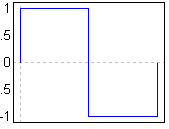
\includegraphics[scale=1.1]{images/haar.png}
\caption{Ondelette de Haar}
\label{haar}
\end{figure}

\subsubsection{Ondelette "chapeau mexicain" :}

On peut définir cette fonction par $\begin{array}{lrcl}
\psi : & \mathbb{R} & \longrightarrow & \mathbb{R} \\
    & t & \longmapsto & \frac{2}{\sqrt{3}}\pi^{-\frac{1}{4}}(1-t^2)e^{-\frac{t^2}{2}} \end{array}$
    
\begin{figure}[!h]
\centering
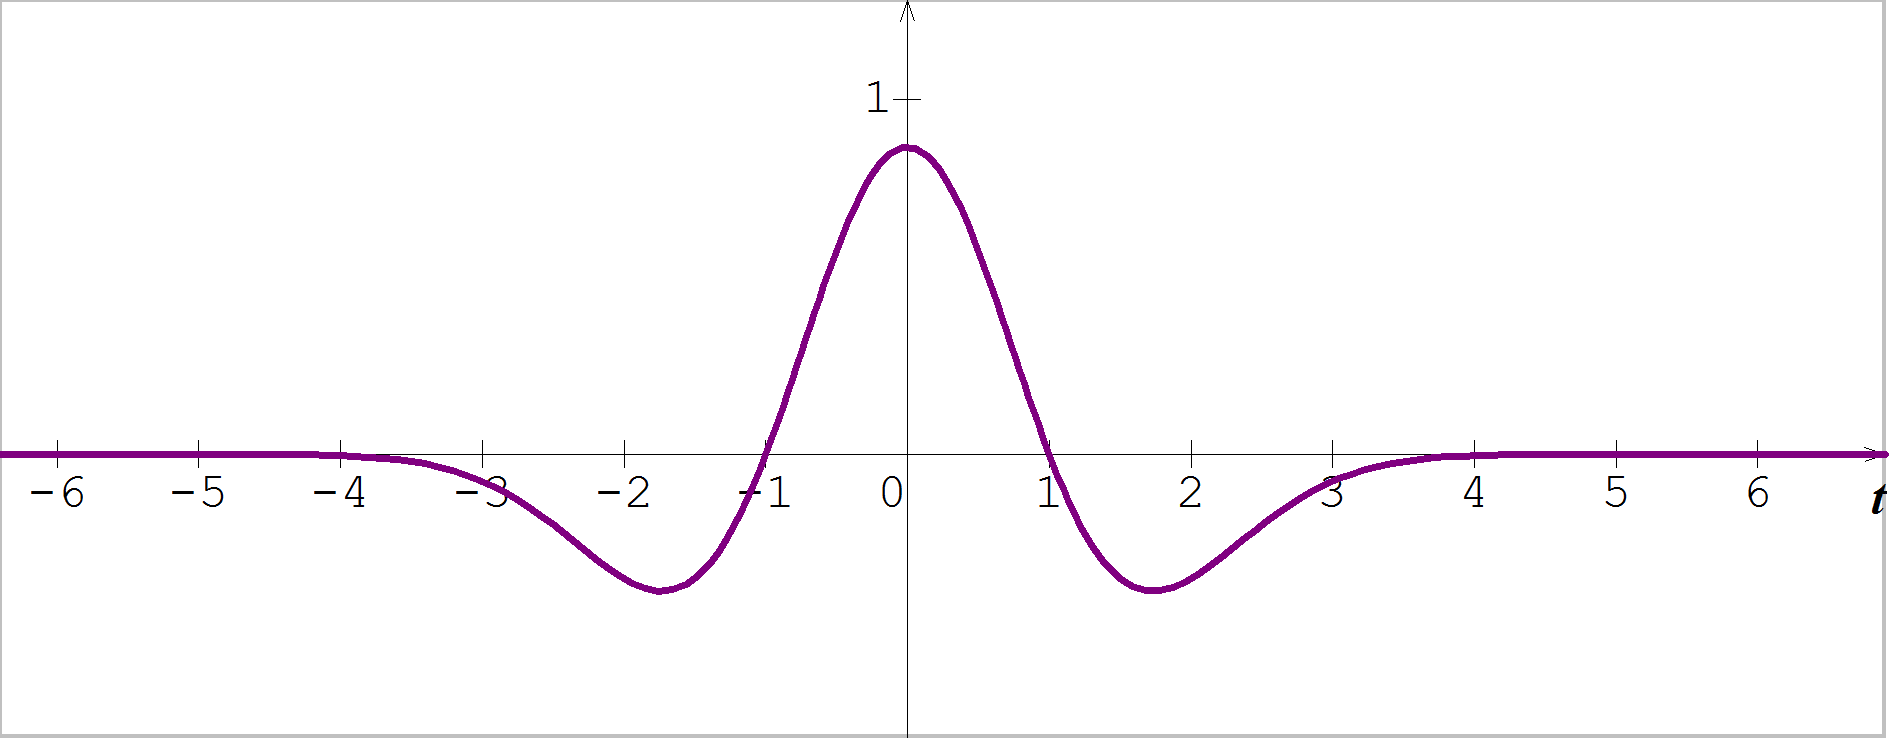
\includegraphics[scale=0.2]{images/chapeau_mexicain.png}
\caption{Ondelette "chapeau mexicain"}
\label{chapmex}
\end{figure}
    
\subsubsection{Ondelette de Morlet :}

On peut définir cette fonction par $\begin{array}{lrcl}
\psi : & \mathbb{R} & \longrightarrow & \mathbb{R} \\
    & t & \longmapsto & \cos(5t)e^{(-\frac{t^2}{2})} \end{array}$
    
\begin{figure}[!h]
\centering
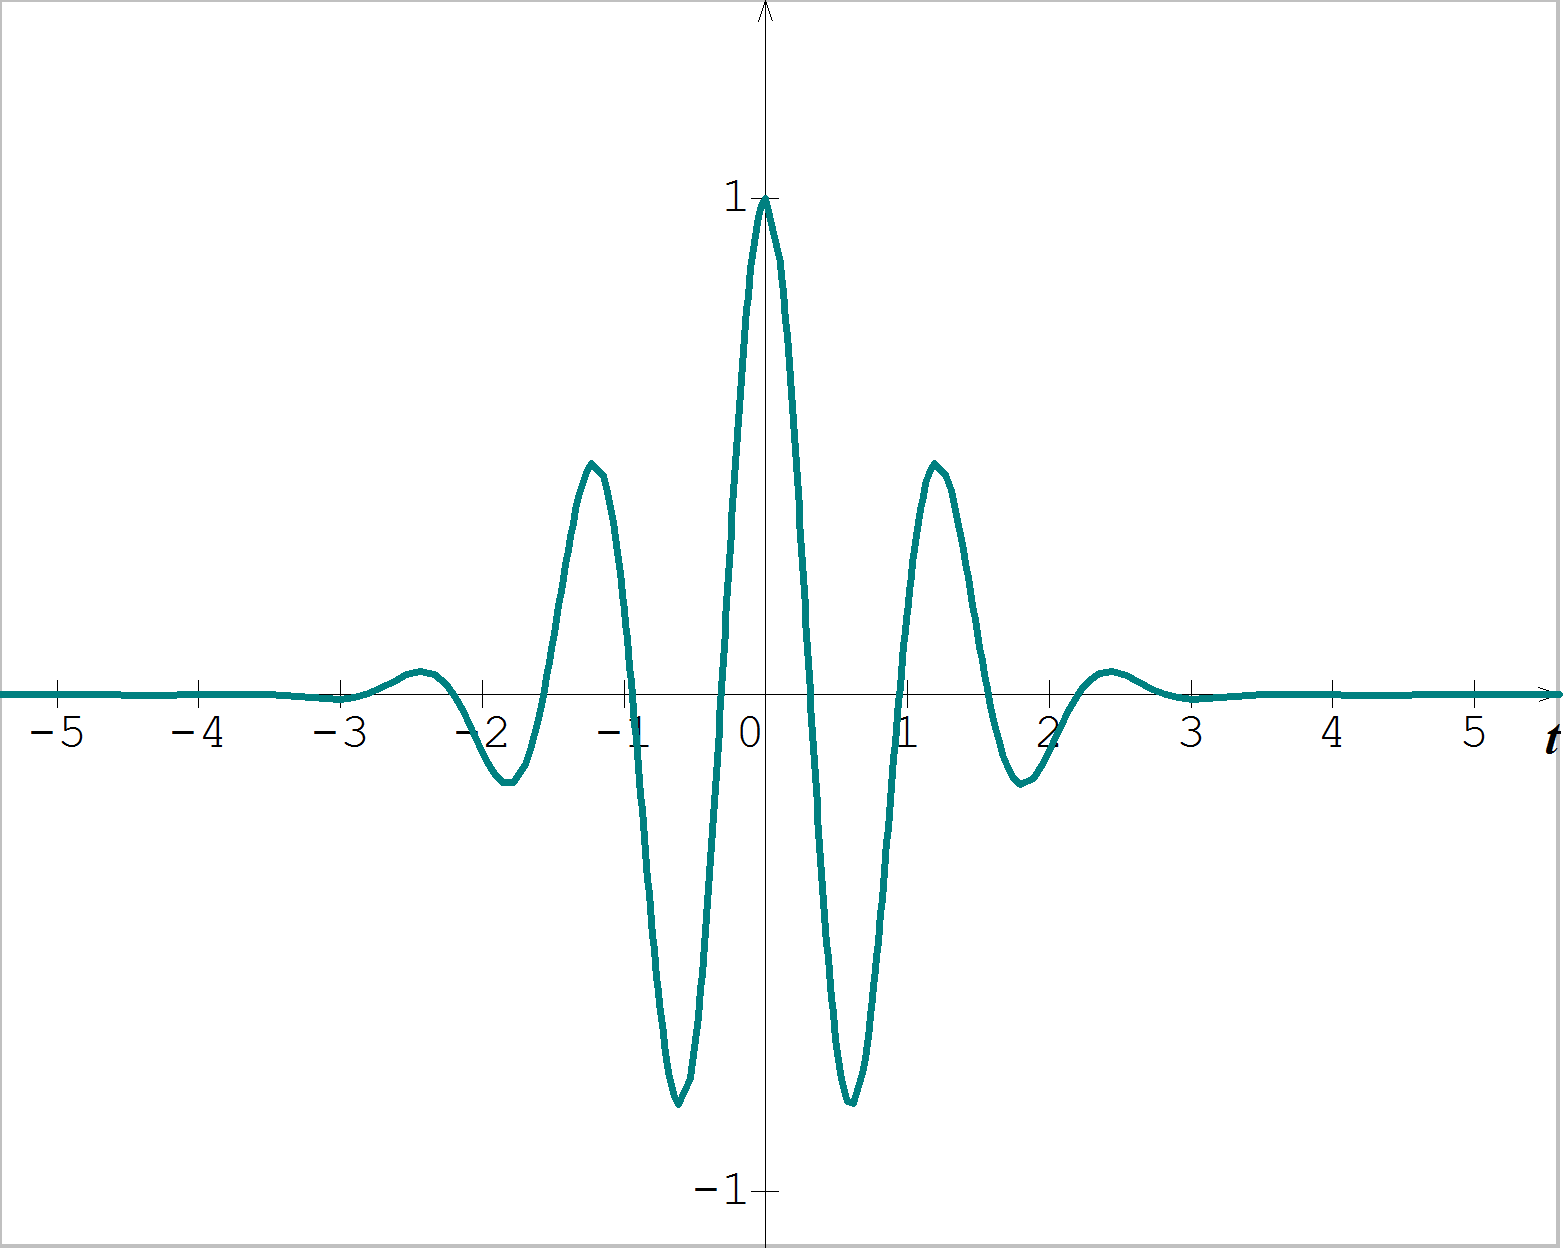
\includegraphics[scale=0.2]{images/morlet.png}
\caption{Ondelette de Morlet}
\label{morlet}
\end{figure}

\pagebreak

\section{Transformation en ondelettes}

La transformée en ondelettes est une transformée linéaire qui décompose un signal en fréquences en conservant une certaine localisation spatiale. Concrètement, le signal de départ est projeté sur un ensemble de fonctions de bases qui varient en fréquence et en espace. 

\subsection{Transformation en ondelette continue}

La transformée en ondelette continue utilise des dilatations et des translations de la fonction ondelette mère. 

\subsubsection*{Définition : produit scalaire}

Soient $f$ et $g$ deux fonctions réelles ; on définit sur le $\mathbb{R}$-espace vectoriel $F$($\mathbb{R}$,$\mathbb{R}$) leur produit scalaire par l’intégrale suivante : \\

$\displaystyle \langle f|g \rangle = \int_{\mathbb{R}} f(x)g(x)dx$ \\

Avec la condition d’admissibilité donnée en première page, la transformée en ondelette continue de la fonction $f$ est définie à facteur constant près comme le produit scalaire de $f$ et de $\psi$. \\

$\displaystyle \mathcal{W}_{(a,b)}(f)= \frac{1}{\sqrt{a}}\int_{-\infty}^{+\infty}f(t)\cdot\psi(\frac{t - b}{a})\cdot dt $ avec $a \in \mathbb{R}_{+}^{*}, b \in \mathbb{R}$ \\

Notons que $a$ permet de donner \textit{l’échelle} (c’est le coefficient de dilatation, de fréquence) et $b$ détermine la position de l’ondelette sur l’axe des temps.

$\frac{1}{\sqrt{a}}$ est le \textit{facteur de normalisation} de l'énergie nécessaire pour que le signal transformé ait la même énergie à toutes les échelles. \\

\textit{Ex} : \textbf{dilatation}.
L’ondelette verte a été dilatée à partir de l’ondelette rouge (ondelette-mère). On a $b = 0$ et $a \neq 1$. \\

\begin{figure}[!h]
\centering
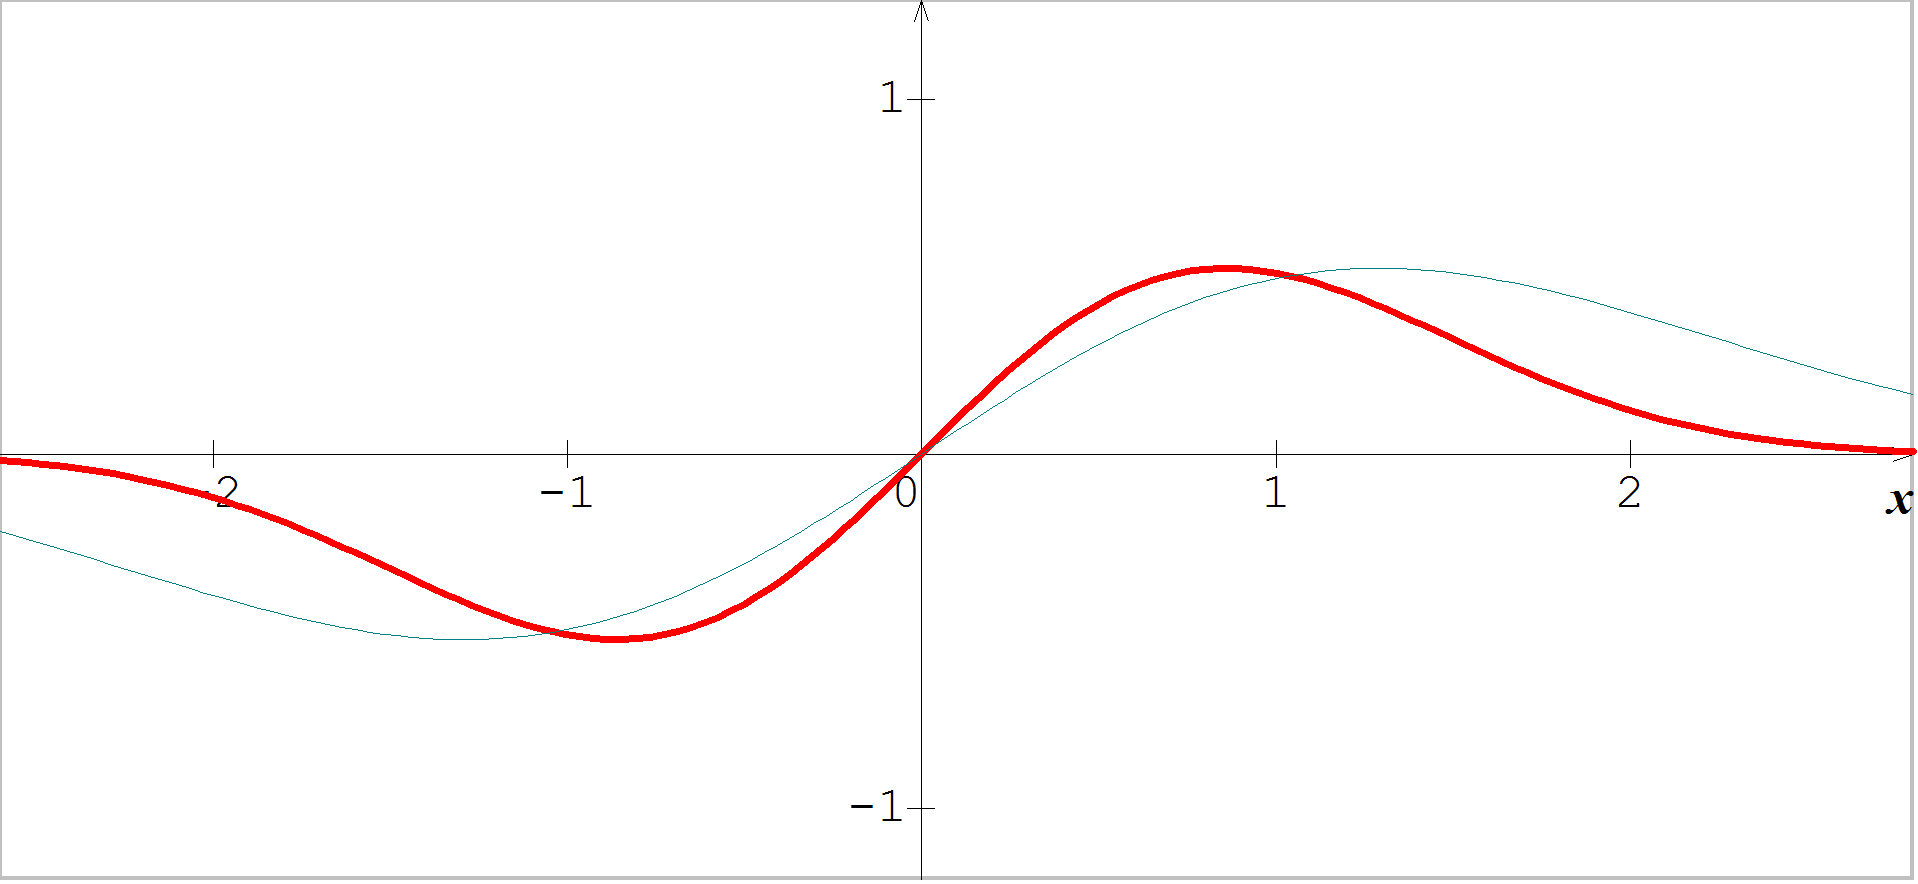
\includegraphics[scale=0.22]{images/dilatation.png}
\caption{Dilatation d'ondelette}
\label{dilat}
\end{figure}

\textit{Ex} : \textbf{translation}.
L’ondelette verte a été translatée à partir de l’ondelette rouge (ondelette-mère). On a $b \neq 0$ 0 et $a = 1$.

\begin{figure}[!h]
\centering
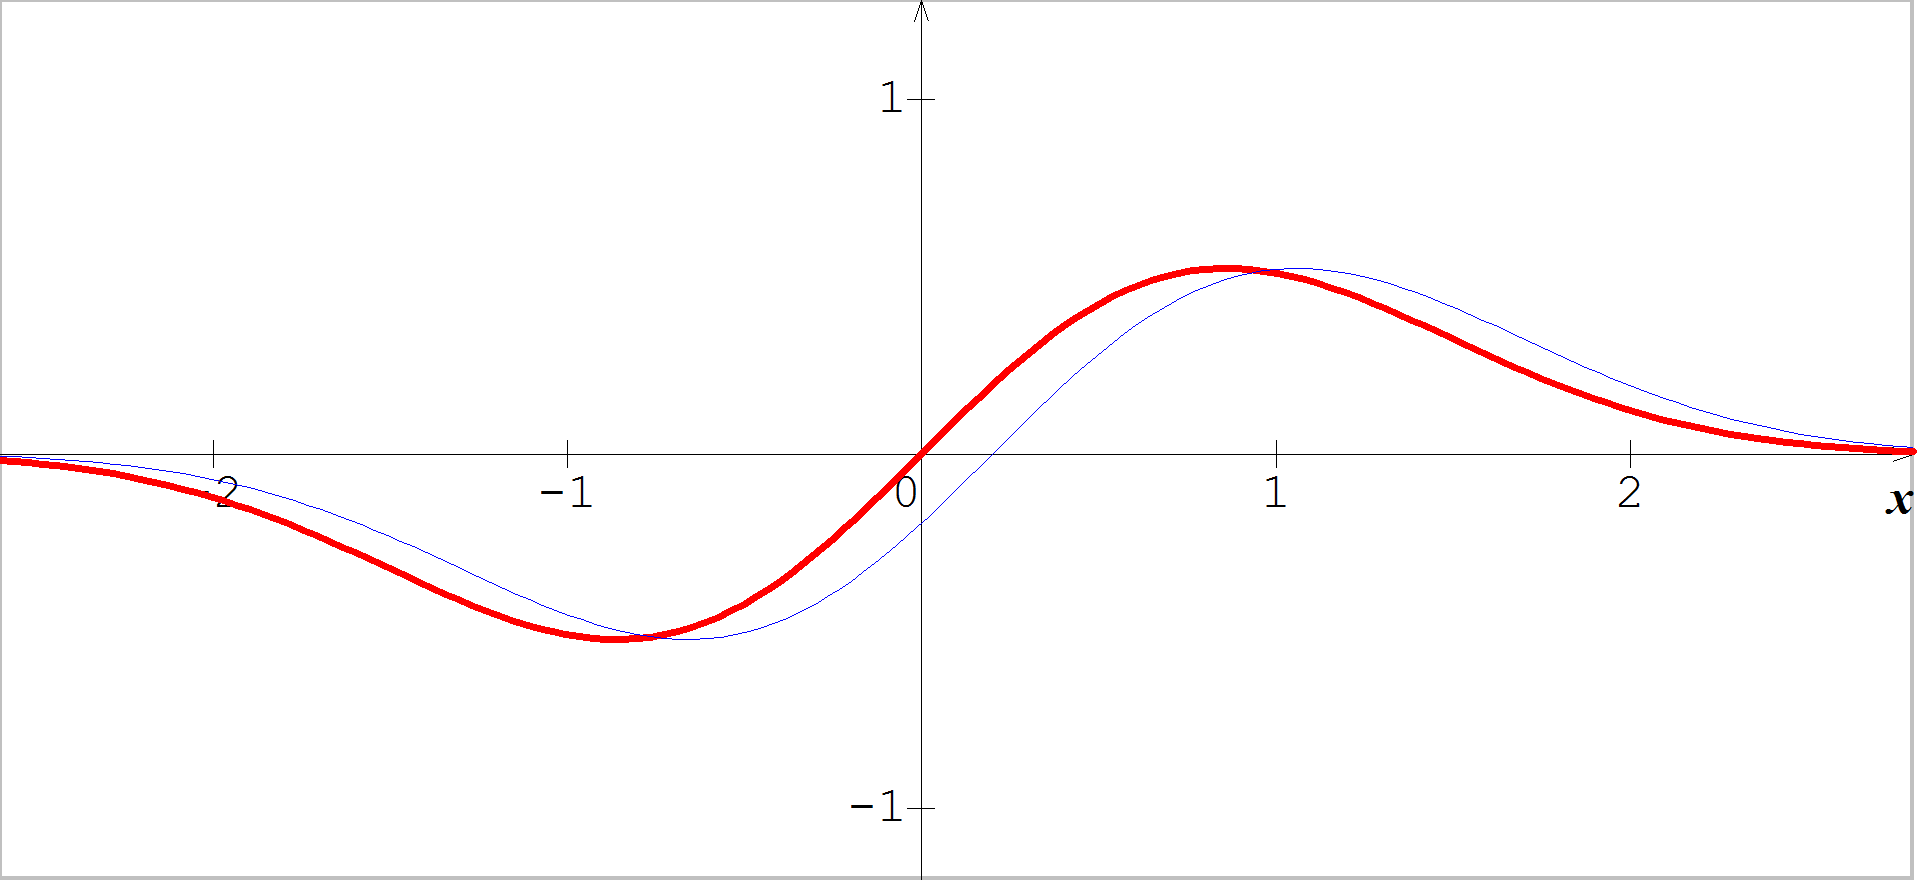
\includegraphics[scale=0.22]{images/translation.png}
\caption{Translation d'ondelette}
\label{translat}
\end{figure}

\subsection{Transformation en ondelettes discrète.}

La transformation en ondelettes discrète qui a été introduite par Morlet se construit à partir de << bases >> de fonctions du type : \\

$\displaystyle f_{t_{0},\Delta{}t}(t) = \frac{1}{\sqrt{\Delta{}t}}f\left(\frac{t-t_0}{\Delta{}t}\right) \text{ avec } \Delta{}t > 0, t_0 \in \mathbb{R}$ \\

$\Delta{}t$ peut être choisi << géométriquement >>; les paramètres de translations $t_0$ et $\Delta{}t$ son proportionnels (c'est-à-dire $\exists k \in \mathbb{R}, t_0 = k\cdot{}\Delta{}t$).

Une gamme d'échelles $\Delta{}t$ utilisée couramment est la gamme d'échelles dyadiques $\frac{1}{2^p}$

On a alors avec $t_0 = k\cdot\Delta{}t$ : \\

$\displaystyle f_{t_{0},\Delta{}t}(t) = 2^{\frac{p}{2}}f(2^{p}\cdot{}x - k)$, c'est-à-dire on peut considérer la famille d'ondelettes $\psi{}_{k,p} = 2^{\frac{p}{2}}\psi{}(2^{p}x - k ), (k,p) \in \mathbb{Z}^2$ \\

Il est intéressant de considérer des familles orthogonales d'ondelettes formant une base hilbertienne de $L^2(\mathbb{R})$ alors toute fonction $f$ de cet espace peut s'écrire 

$\displaystyle f = \sum_{(k,p) \in \mathbb{Z}^2}f_{k,p}\psi{}_{k,p}$ où les $f_{k,p} = \langle{}f|\psi_{k,p}\rangle$ sont appelés coefficients d'ondelettes.

La transformation en ondelettes discrète est presque naturellement associée à des algorithmes plus efficaces et plus rapides que des algorithmes du type FFT qui utilisent la transformée de Fourier.

Une famille d’ondelettes par exemple couramment utilisée dans la transformation en ondelettes discrète est la famille infinie des ondelettes orthogonales de Daubechies : c’est une des familles d’ondelettes les plus performantes.

\subsection{Comparaison avec la transformation de Fourier}


Un des avantages de la transformation par les ondelettes (en comparaison avec la transformation de Fourier), c'est que le fait de modifier ou de supprimer un des coefficients de la transformée d'un signal ne va en rien dégrader le signal. \\
En outre, les algorithmes de transformation en ondelettes 2D s'appliquent à la totalité de l'image et non pas à des blocs de pixels comme par exemple les algorithmes type FFT, ce qui permet d'éviter les carrés uniformes lorsque le taux de compression est relativement élevé. \\
Enfin, l'utilisation d'une ondelette réversible permet une compression sans perte de données. \\ \\ \\
\begin{figure}[!h]
\centering
<<<<<<< HEAD
\includegraphics[scale=0.4]{comparaison.jpg}
=======
\includegraphics[scale=0.4]{images/comparaison.jpg}
>>>>>>> d5245ec323332736ffd68589bb833e4bf5a5f8bb
\caption{Comparaison des méthodes de compression}
\end{figure} \\
La figure ci-dessus montre les résultats de deux compressions de la même image de départ, l'une utilisant la transformation de Fourier (à gauche), l'autre utilisant la transformation en ondelettes (à droite). \\ \\
Enfin, le coût d'un algorithme utilisant les ondelettes, c'est-à-dire le nombre d'opérations à effectuer, est en $O(N)$, ce qui est mieux que le coût des meilleurs algorithmes type FFT en $O(N\log N)$.




\section{La théorie de l'analyse multirésolution, un outil pour la construction de bases d'ondelettes}

Pour construire des bases d'ondelettes orthonormées, les théoriciens Mallat et Meyer ont introduit la notion d'analyse multirésolution.

\subsection{Définition d'une analyse multirésolution.}

Une analyse multirésolution est une suite $\{V_k\}_{k\in\mathbb{Z}}$ de sous-espaces fermés de $\mathcal{L}^2(\mathbb{R})$ tels que : \\

\begin{itemize}
\item $\forall{}(k,l) \in \mathbb{Z}^2, f \in V_k \Leftrightarrow f(\cdot - 2^{k}l) \in V_k $ (propriété d'invariance par translation)

\item $\forall k \in \mathbb{Z}, V_{k+1} \subset V_k$

\item $\forall k \in \mathbb{Z}, f \in V_k \Leftrightarrow f(\frac{\cdot}{2}) \in V_{k+1}$

\item $\displaystyle \lim_{j \to \infty} V_k = \bigcap_{k\in\mathbb{Z}}V_k = \textrm{Ø} $

\item $\displaystyle \lim_{j \to -\infty} V_k = \overline{\bigcap_{k\in\mathbb{Z}}V_k} = \mathcal{L}^2(\mathbb{R}) $ où la notation $\bar{A}$ désigne l'adhérence de $A$.

\item $\exists\phi, \{\phi(\cdot - n)\}_{n \in \mathbb{Z}}$ forme une base orthonormée de $V_0$. $\phi$ est appelée fonction d'échelle associée à l'analyse multirésolution
\end{itemize}

\subsection{Intéret d'une analyse multirésolution}

La fonction $\phi$ permet notamment la connaissance de la suite $\{V_k\}_{k\in\mathbb{Z}}$ et ainsi la déduction d'une base orthonormée de $V_k$ pour tout $k \in \mathbb{Z}$. On peut alors définir une ondelette associée à l'analyse multirésolution : il s'agira de toute fonction $\psi$ qui forme avec ses translatées entières une base orthonormée de $W_0$, supplémentaire orthogonal de $V_1$ dans $V_0$. En effet, il découle de la définition de $W_k$ que $\displaystyle \mathcal{L}^2(\mathbb{R}) = \overline{\bigoplus{}_{k\in\mathbb{Z}}W_k}$. \\

Par suite, la famille $ \left\{ {\displaystyle \frac{1}{\sqrt{2^{m}}}\psi\left(\frac{.-2^{m}n}{2^{m}}\right)}\right\}$ forme une base orthonormée de $\mathcal{L}^2(\mathbb{R})$.

Les espaces $W_k$ pour $k\in\mathbb{Z}$ sont appelés espaces des détails. Ils ne forment pas une famille d'espaces emboîtés mais les propriétés d'échelles et d'invariance par translation sont conservées. En effet, pour $k \in \mathbb{Z}, W_{k-1}$ est orthogonal à $V_{k-1}$, d'où $W_{k-1}$ orthogonal à $W_k$ en vertu de l'égalité $\displaystyle \mathcal{L}^2(\mathbb{R}) = \overline{\bigoplus{}_{k\in\mathbb{Z}}W_k}$.



\section{Algorithme de décomposition en ondelettes de Stéphane Mallat (1989)}

\subsection{Principe}

C’est un algorithme linéaire qui fait appel à un sous-échantillonnage. Concrètement, on procède à une décomposition par projections successives (c’est-à-dire de manière récursive) sur deux sous-espaces orthogonaux, l’un donnant l’allure générale de l’image (il s'agira de l'image en résolution moitié) et l’autre les détails. 
L’algorithme de Mallat a cependant le défaut de ne pas être invariant par translation.

On peut donner une démonstration mathématique de cet algorithme ; ici, pour simplifier, on va se limiter au cas particulier de décomposition d’un signal par les ondelettes de Haar.


\subsection{Démonstration dans un cas simple : le cas des ondelettes de Haar.}

La démonstration suivante montre comment on calcule les coefficients des ondelettes de Haar : on est bien évidemment dans le cadre d'une transformation en ondelettes discrètes.

\subsubsection{Introduction et définition des notations}

Considérons un signal échantillonné régulièrement sur [0,1] en $2^p$ points notés $x_{k}$ avec $x_{k} = \frac{k}{2^p}$.

On associe à cet échantillon une fonction $f$ définie par $f(x) = \begin{cases}
     f_{k} \text{ si } x \in I_{k} = [x_{k},x_{k+1}[\\
     0 \text{ sinon }
   \end{cases}$.
Quand l'échantillonnage varie, $f$ varie en décrivant l'ensemble $\mathbb{K}_{p}$ des fonctions constantes sur chacun des intervalles $I_{k}$ et nulles sur $\mathbb{K} \setminus [0,1]$. \\

$F$($\mathbb{R}$,$\mathbb{R}$), ensemble des fonctions réelles à valeurs réelles, est un $\mathbb{R}$-espace vectoriel et on montre facilement que $\mathbb{K}_{p}$ est un sous-espace vectoriel de $F(\mathbb{R},\mathbb{R})$. \\

De plus, pour $p \in \mathbb{N}$, on a $\mathbb{K}_{0} \subset \mathbb{K}_{1} \subset .. \subset \mathbb{K}_{p} \subset \mathbb{K}_{p+1} \subset ... $ ce qui montre $\bigcup\limits_{p \in \mathbb{N}}\mathbb{K}_{p}$ est un sous-espace vectoriel de $F(\mathbb{R},\mathbb{R})$.

\uppercase{à} partir de la fonction de Haar $H$, on définit la fonction $H_{p,k}$ par $H_{p,k}(x) = H(2^{p}x - k). (p,k) \in \mathbb{N}^2$.

\textit{[Pour alléger l’écriture et les calculs, on peut comme ici choisir d’omettre le facteur }$2^\frac{p}{2}$ devant $ H(2^{p}x - k)$.] \\

Soit la fonction définie par \[
 h_{p,k}(x) = \begin{dcases*}
        1 \text{ si } x \in I_{k} = [\frac{k}{2^p},\frac{k+1}{2^p}] \\ 
        0 \text{ sinon }
        \end{dcases*}
 = h(2^{p}x - k) \] (avec $h$ définie comme la fonction de Haar mais associant 1 quel que soit $x \in [0,1]$.). \\

Or toute fonction $f$ de $\mathbb{K}_{p}$ se décompose de manière unique sous la forme : \\

$\displaystyle f = \sum_{k = 0}^{2^p - 1} f_{k}h_{p,k} = f_{0}h_{p,0} + f_{1}h_{p,1} + ... + f_{2^p - 1}h_{p,2^p - 1}$ \\

On a bien $\forall x \in [0,1[, f(x) = f_0 \times \begin{cases} 1 \text{ si } x \in I_0 \\ 0 \text{ sinon } \end{cases}
+ f_1 \times \begin{cases} 1 \text{ si } x \in I_1 \\ 0 \text{ sinon } \end{cases}
+ ... +
f_{2^p - 1} \times \begin{cases} 1 \text{ si } x \in I_{2^p - 1} \\ 0 \text{ sinon } \end{cases} $.\\

D'où $(h_{p,0},h_{p,1},...,h_{p,2^p -1})$ est une base de $\mathbb{K}_p$.\\


Avec $F(\mathbb{R},\mathbb{R})$ muni du produit scalaire défini en \textit{définition 2}, on a : \\

\begin{itemize}

\item Si $k \neq k'$ :

$\displaystyle \langle h_{p,k}|h_{p,k'} \rangle = \int_{0}^{1} h_{p,k}(x)\cdot{}h_{p,k'}(x) = \int_0^1 0\cdot{}dx = 0$ \\

\item Si $k = k'$ :

\begin{align*} \displaystyle
\langle h_{p,k}|h_{p,k'} \rangle &= \int_{0}^{1} (h_{p,k}(x))^2 dx \\
 &= \int_{0}^{x_k} h_{p,k}(x))^2 dx + \int_{x_k}^{x_{k+1}} h_{p,k}(x))^2 dx + \int_{x_{k+1}}^{1} h_{p,k}(x))^2 dx  \\
\displaystyle &= \int_0^{x_k} 0^2 dx + \int_{x_k}^{x_{k+1}} 1^2 dx + \int_{x_{k+1}}^{1} 0^2 dx = 0 + [x]_{x_k}^{x_{k+1}} + 0 = x_{k+1} - x_k  \\
\displaystyle &= \frac{1}{2^p} \\
\end{align*} 
\end{itemize}

Ainsi la base $(h_{p,0},h_{p,1},...,h_{p,2^p -1})$ est une base orthogonale ; ce qui fait des espaces $\mathbb{K}_p$ des espaces euclidiens.


\subsubsection{Propriété mathématique : Orthogonalité dans les espaces euclidiens}
\paragraph{\uppercase{é}noncé}
Soient $E$ un espace euclidien de dimension $n \geq 1$, $\langle .| .\rangle$ son produit scalaire et $F$ un sous-espace vectoriel de $E$.

Alors $F$ admet un supplémentaire orthogonal dans $E$ et ce supplémentaire est unique. On le note : $F^{\perp}$.
 \\
 \\
\paragraph{Démonstration} :

\begin{itemize}

\item Existence :

\begin{itemize}

\item Si $F = \{0_E\}$, on a $E = F \oplus E$ de manière immédiate. De plus, si $y \in F, y = 0_E$ et $\forall x \in E, \langle x|0_E \rangle = 0 $. D'où E est un supplémentaire orthogonal à $F$. \\

\item Si $F = E$, par un raisonnement analogue, on trouve que $\{0_E\}$ est un supplémentaire orthogonal à $F$. \\

\item Si $F \neq \{0_E\}$ et $F \neq E$, on considère $(e_i)_{1\leq{}i\leq{}p}$ une base orthonormale de $F$ avec $p =$ dim $F \in \mathbb{N}^{*}.$ \\

L'ensemble $F^{\perp} = \{ x \in E | \forall y \in F, \langle x|y \rangle = 0 \}$ est par définition orthogonal à $F$. \\

Soit $x \in E$.

$\exists (\lambda{}_{1}, ..., \lambda{}_{p}) \in \mathbb{R}^p , x =\displaystyle \sum_{k = 1}^{p} \lambda{}_{k}e_k + (x - \sum_{k = 1}^{p} \lambda{}_{k}e_k)$

Or le premier vecteur de la somme est dans $F$. Donc le second entre parenthèses appartient à $F^{\perp}$ si et seulement si 

$\displaystyle \forall k \in [|1,p|], \langle e_k | x -\displaystyle \sum_{k = 1}^{p}\lambda{}_{k}e_k \rangle = 0$, c'est-à-dire $\lambda_{k} = \langle e_k | x \rangle$

Avec $x$ écrit de la manière suivante, on établit ainsi que  $E = F + F^{\perp}$.

$\displaystyle x = \sum_{k = 1}^p \langle e_k | x \rangle{}\cdot{}e_k + (x - \sum_{k = 1}^p \langle e_k | x \rangle{}\cdot{}e_k)$

On a aussi immédiatement $F \cap F^{\perp} = \{0_E\}$, ce qui établit $E = F \oplus F^{\perp}$ et ainsi l'existence d'un supplémentaire orthogonal à $F$ 
\end{itemize}

\item Unicité :

Soit $G$ un sous-espace vectoriel supplémentaire de $F$ dans $E$ et orthogonal à $F$.

On a déjà $G \subset F^{\perp}$ puisque tous les vecteurs de G sont orthogonaux à tous les vecteurs de $F$.

De plus, dim $G$ = dim $E -$ dim $F$ = dim $F^{\perp}$ car $\begin{dcases} E = F \oplus F^{\perp} \\ E = F \oplus G \end{dcases}$; on en déduit $G = F^{\perp}$ et l'unicité du supplémentaire orthogonal. \\
\end{itemize}

\subsubsection{Utilisation de la propriété : décomposition orthogonale en somme directe.}

Soit donc $\mathbb{S}_{p}$ le supplémentaire orthogonal de $\mathbb{K}_p$ dans $\mathbb{K}_{p+1}$. \\

On a $\mathbb{K}_{p+1} = \mathbb{S}_{p} \oplus \mathbb{K}_p$. D'où de proche en proche on arrive à :

$\mathbb{K}_{p+1} = \mathbb{S}_{p} \oplus \mathbb{S}_{p-1} \oplus \mathbb{S}_{p-2} \oplus ... \oplus \mathbb{S}_{0} \oplus \mathbb{K}_{0}$, soit encore $\mathbb{K}_p = \mathbb{K}_0 \oplus{}_{i = 0}^{p-1} \mathbb{S}_{i	} $ \\

On a défini à partir de $\mathcal{H}$ la fonction $H_{p,k}$ par $H_{p,k}(x) = \mathcal{H}(2^{p}x - k )$; $(p,k) \in \mathbb{N}^2$.

On alors $H_{p,k}(x) =  \begin{dcases} 1 \text{ si } x \in [\frac{k}{2^p};\frac{k + \frac{1}{2}}{2^p}[ \\ 
-1 \text{ si } x \in [\frac{k + \frac{1}{2}}{2^p};\frac{k + 1}{2^p}[ \\
0 \text{ dans les autres cas } \end{dcases}$.

Facilement, on montre que $(h_{p,1},h_{p,0},...,h_{p,2^p - 1},H_{p,0},H_{p,1},...,H_{p,2^p - 1})$ forme une base de $\mathbb{K}_{p+1}$.

De plus, on a :

\begin{itemize}

\item Si $k \neq k'$

\begin{align*}
\langle h_{p,k}|H_{p,k'} \rangle &= \int_{0}^1 h_{p,k}(x)\cdot{}H_{p,k'}(x)\cdot{dx} \\ 
&= \int_{0}^{x_k} 0 dx + \int_{x_k}^{x_{k+1}} 1\cdot{}0dx + \int_{x_{k+1}}^{x_{k'}} 0dx + \\
 &\int_{x_{k'}}^{\frac{x_{k'} + x_{k'+1} }{2}} 0\cdot{}1dx + \int_{\frac{x_{k'} + x_{k'+1} }{2}}^{x_{k'+1}} 0(-1)dx + \int_{x_{k'+1}}^{1} 0.dx \\
&= 0
\end{align*} 
\item Si $k =k'$

\begin{align*}
 \langle h_{p,k}|H_{p,k'} \rangle &= \int_{0}^1 h_{p,k}(x)\cdot{}H_{p,k'}(x)\cdot{dx} \\
&= \int_{0}^{x_k} 0dx + \int_{x_k}^{x_{k+1}} 1\cdot{}H_{p,k}(x)dx + \int_{x_{k+1}}^{1} 0\cdot{}dx \\
&= \int_{x_{k'}}^{\frac{x_{k'} + x_{k'+1} }{2}} 1dx + \int_{\frac{x_{k'} + x_{k'+1} }{2}}^{x_{k'+1}} -1dx \\
&= 0 . \\
\end{align*}
\end{itemize}

De ce qui précède, il résulte que $(h_{p,1},h_{p,0},...,h_{p,2^p - 1},H_{p,0},H_{p,1},...,H_{p,2^p - 1})$ forme une base orthogonale de $\mathbb{K}_{p+1}$.

Alors le système $(H_{p,0}, H_{p,1},..., H_{p,2^p - 1},)$ est une base orthogonale de l'orthogonal $\mathbb{S}_{p}$ de $\mathbb{K}_{p}$ dans $\mathbb{K}_{p+1}$.

De plus, on peut déjà remarquer :

$\displaystyle \langle H_{p,k}|H_{p,k} \rangle = \int_0^1 (H_{p,k}(x))^{2}\cdot{}dx = \int_{x_{k'}}^{\frac{x_{k'} + x_{k'+1} }{2}} 1^{2}\cdot{}dx + \int_{\frac{x_{k'} + x_{k'+1} }{2}}^{x_{k'+1}} (-1)^{2}\cdot{}dx = \frac{1}{2^p} $ \\


-Soit un signal $\Psi{}_{p} \in \mathbb{K}_{p}$. \\ Alors $\displaystyle \exists{}! (\Psi{}_{p,0},\Psi{}_{p,1},...,\Psi{}_{p,2^p - 1},) \in \mathbb{R}^{2^p}, \Psi{}_{p} = \sum_{k=0}^{2^p - 1} \Psi{}_{p,k}h_{p,k}$.

Puisque $\mathbb{K}_{p} = \mathbb{K}_{p-1} \oplus \mathbb{S}_{p-1}, \exists{}!(\Psi{}_{p-1},d_{p-1}) \in \mathbb{K}_{p-1} \times \mathbb{S}_{p-1}, \Psi{}_p = \Psi{}_{p-1} + d_{p-1} $. \\

Et on peut décomposer $\Psi{}_{p-1}$ et $d_{p-1}$ comme suit :

$\displaystyle \Psi{}_{p-1} = \sum_{k=0}^{2^p - 1} \Psi{}_{p-1,k}h_{p-1,k}$ et $d_{p-1} =\displaystyle \sum_{k=0}^{2^p - 1} d_{p-1,k}H_{p-1,k}$. \\

\subsubsection{\uppercase{é}tape principale de l'algorithme : passage à la résolution inférieure, détermination des coefficients à la résolution inférieure.}

-Déterminons les $\Psi{}_{p-1,k}$ et $d_{p-1,k}$ :

\paragraph{Premières égalités}
L'orthogonalité de la base $(h_{p,1},h_{p,0},...,h_{p,2^p - 1},H_{p,0},H_{p,1},...,H_{p,2^p - 1})$ avec $\Psi{}_{p} = \Psi{}_{p-1} + d_{p-1}$ et les résultats précédents sur les produits scalaires amène à : \fbox{$\langle \Psi{}_{p}|h_{p-1,k} \rangle = \frac{\Psi{}_{p-1,k}}{2^{p-1}}$ }et \fbox{$\langle \Psi{}_{p}|H_{p-1,k} \rangle = \frac{d_{p-1,k}}{2^{p-1}}$}. \\

\subparagraph*{Démonstration} 

On a \begin{align*}
 \langle\Psi{}_{p}|h_{p-1,k} \rangle &= \langle \Psi{}_{p-1}|h_{p-1}\rangle + \langle d_{p-1}|h_{p-1,k} \rangle  \text{ par linéarité du produit scalaire.} \\
 &= \sum_{i \neq k} \Psi{}_{p-1,i} \langle h_{p-1,i}|h_{p-1,k} \rangle + \Psi{}_{p-1,k} \langle h_{p-1,k}|h_{p-1,k} \rangle + \sum_{i=0}^{2^{p-1} - 1} d_{p-1,i}\langle H_{p-1,i}|h_{p-1,k} \rangle  \\
 &= \sum_{i \neq k} \Psi{}_{p-1,i}\cdot{}0 + \frac{\Psi{}_{p-1,k}}{2^{p-1}} + \sum_{i=0}^{2^{p-1} - 1} d_{p-1,i}\cdot{}0 = \frac{\Psi{}_{p-1,k}}{2^{p-1}} 
 \end{align*}

Et on a 
\begin{align*} \displaystyle
 \langle\Psi{}_{p}|H_{p-1,k} \rangle &= \langle \Psi{}_{p-1}|H_{p-1}\rangle + \langle d_{p-1}|h_{p-1,k} \rangle  \\
&= \sum_{i=0}^{2^{p-1}-1} \Psi{}_{p-1,i}\langle h_{p-1,i}|H_{p-1,k}\rangle + \sum_{i \neq k}d_{p-1,i}\langle{}H_{p-1,i}|H_{p-1,k} \rangle + d_{p-1,k}\langle{}H_{p-1,k}|H_{p-1,k}\rangle  \\
&= \sum_{i=0}^{2^{p-1}-1}\Psi{}_{p-1,i}\cdot{}0 + \sum_{i \neq k}d_{p-1,i}\cdot{}0 + d_{p-1,k}\langle{}H_{p-1,k}|H_{p-1,k}\rangle \\ &= \frac{d_{p-1,k}}{2^{p-1}}
\end{align*} \\

\paragraph{Secondes égalités}

D'autre part, on peut montrer \fbox{$\displaystyle \langle{}\Psi{}_{p}|h_{p-1,k}\rangle = \frac{\Psi{}_{p,2k} + \Psi{}_{p,2k + 1} }{2^p}$} et \fbox{$\displaystyle \langle{}\Psi{}_{p}|H_{p-1,k}\rangle = \frac{\Psi{}_{p,2k} - \Psi{}_{p,2k + 1} }{2^p}$} \\


\subparagraph*{Démonstration} 

On a $\displaystyle \langle{}h_{p,k}|h_{p-1,k'}\rangle = \int_0^1 h_{p,k}(x)\cdot{}h_{p-1,k'}(x)\cdot{}dx = \int_{x_k}^{x_{k+1}}h_{p-1,k'}(x)\cdot{}dx$ \\

Or, on sait par définition que \[ h_{p-1,k'}(x)= \begin{dcases} 1 \text{ si }x \in [\frac{k'}{2^{p-1}};\frac{k'+1}{2^{p-1}} ] \\
0 \text{ sinon } \end{dcases} \]\\
D'où :
\[ \begin{dcases}
\langle{}h_{p,k}|h_{p-1,k'}\rangle = \int_{x_k}^{x_{k+1}}1\cdot{}dx
= \frac{1}{2^p} \text{ si } \frac{k'}{2^{p-1}} \leq x_k \leq x_{k+1} \leq \frac{k'+1}{2^{p-1}}, \text{ ou encore } k \in \{2k',2k'+1\}\\ 
\langle{}h_{p,k}|h_{p-1,k'}\rangle = \int_{x_k}^{x_{k+1}0\cdot{}dx = 0 si k \notin \{2k',2k'+1\}}
\end{dcases} \]

On a de même \\
 $\displaystyle \langle{}h_{p,k}|H_{p-1,k'}\rangle = \int_0^{1}h_{p,k}(x)\cdot{}H_{p-1,k'}(x)\cdot{}dx = \int_{x_k}^{x_{k+1}}H_{p-1,k'}(x)\cdot{}dx$

On sait par définition que \[ H_{p-1,k'}(x) = \begin{dcases} 
1 \text{ si } x \in [\frac{k'}{2^{p-1}};\frac{k'+\frac{1}{2}}{2^{p-1}} ] \\
-1 \text{ si } x \in []\frac{k'+\frac{1}{2}}{2^{p-1}};\frac{k'+1}{2^{p-1}} ] \\
0 \text{ sinon }
\end{dcases}
\] D'où :

\[ \begin{dcases}
\langle{}h_{p,k}|H_{p-1,k'}\rangle = \int_{x_k}^{x_{k+1}}1\cdot{}dx = \frac{1}{2^p} \text{ si } \frac{k'}{2^{p-1}} \leq x_k \leq x_{k+1} \leq \frac{k'+\frac{1}{2}}{2^{p-1}}, \text{ ou encore } k = 2k' \\
\langle{}h_{p,k}|H_{p-1,k'}\rangle = \int_{x_k}^{x_{k+1}}-1\cdot{}dx = -\frac{1}{2^p} \text{ si } \frac{k'+\frac{1}{2}}{2^{p-1}} \leq x_k \leq x_{k+1} \leq \frac{k'+1}{2^{p-1}}, \text{ soit } k = 2k'+1 \\
\langle{}h_{p,k}|H_{p-1,k'}\rangle = \int_{x_k}^{x_{k+1}}0\cdot{}dx = 0 \text{ si } k \notin \{2k',2k'+1\}
\end{dcases}
\]

\uppercase{à} partir de cela, il est facile de décomposer comme suit et d'obtenir les résultats :

\begin{itemize}
\item \begin{align*}\displaystyle \langle \Psi{}_{p}|h_{p-1,k}\rangle &=  \langle \sum_{k=0}^{2^{p}-1}\Psi{}_{p,k}h_{p,k}|h_{p-1,k}\rangle \\ &=  \sum_{i\notin{}\{2k',2k'+1\}}\Psi{}_{p,i}\langle{}h_{p,i}|h_{p-1,k}\rangle + \sum_{i\notin{}\{2k',2k'+1\}}\Psi{}_{p,i}\langle{}h_{p,i}|h_{p-1,k}\rangle  \\ 
&= 0 + \Psi{}_{p,2k}\cdot{}\frac{1}{2^p} + \Psi{}_{p,2k+1}\cdot{}\frac{1}{2^p} 
\end{align*} 

\item \begin{align*} \displaystyle \langle \Psi{}_{p}|H_{p-1,k}\rangle &= \langle \sum_{k=0}^{2^{p}-1}\Psi{}_{p,k}h_{p,k}|H_{p-1,k}\rangle \\ &= 
 \sum_{i\notin{}\{2k',2k'+1\}}\Psi{}_{p,i}\langle{}h_{p,i}|H_{p-1,k}\rangle + \sum_{i\notin{}\{2k',2k'+1\}}\Psi{}_{p,i}\langle{}h_{p,i}|h_{p-1,k}\rangle  \\ 
&= 0 + \Psi{}_{p,2k}\cdot{}\frac{1}{2^p} + \Psi{}_{p,2k+1}\cdot{}\frac{-1}{2^p}
\end{align*} \\


\end{itemize}

\paragraph{Conclusion}

On obtient finalement avec les égalités encadrées les équations d'échelles suivantes. \\

\[ \begin{dcases} \Psi{}_{p-1,k} = \frac{\Psi{}_{p,2k} + \Psi{}_{p,2k}}{2}  \| (\Psi{}_{p-1,k})_{k\in{}[|0;2^{p-1}-1|]} \text{est la famille des coefficients d'approximation à la résolution} 2^{p-1} \\ 
d_{p-1,k} = \frac{\Psi{}_{p,2k} - \Psi{}_{p,2k}}{2}  \| (d_{p-1,k})_{k\in{}[|0;2^{p-1}-1|]} \text{est la famille des coefficients d'ondelettes}
\end{dcases} \] 

Ainsi, lorsqu’on connaît les coefficients d’ondelettes à un niveau de résolution $p$, on peut aisément déterminer ceux du niveau $p-1$ et l’égalité des sous-espaces vectoriels en somme directe se comprend par :

$$ \underbrace{\mathbb{K}_p}_{\text{Signal à la résolution } 2^p}
= \underbrace{\mathbb{K}_{p-1}}_{\text{Signal à la résolution } 2^{p-1}} \oplus 
\underbrace{\mathbb{S}_{p-1}}_\text{Détails (ou pertes)} $$

L’intérêt principal de cet algorithme est qu’il permet de passer d’un échantillon de taille $2^p$ à un nouvel échantillon principal de taille $2^{p-1}$ et un échantillon de taille $2^{p-1}$ en utilisant que des sommes ou des différences.


\subsection{Schématisation de l'algorithme de Mallat (compression d'un signal $\Psi{}_{p}$ par des ondelettes)} 

\begin{tabular}{cccc}
           &             & Etape 1      & \\
$\Psi{}_{p}$ & $\rightarrow$ & $\Psi{}_{p-1}$ & \\
           & $\searrow$    & $d_{p-1}$      & (détails)
\end{tabular} \\

En réitérant le processus jusqu’à la dernière étape (étape $p$), on obtient la configuration suivante : \\


\begin{tabular}{ccccccccc}
           &             & Etape 1      & 			  & Etape 2     & & & & Etape p \\
$ \Psi{}_{p}$ & $ \rightarrow$ & $ \Psi{}_{p-1}$ & $ \rightarrow$ & $ \Psi{}_{p-2}$ & $ \rightarrow$ & ... & $ \rightarrow$ & $ \Psi{}_0$ \\
           & $ \searrow$    & $ d_{p-1} $      & $ \searrow$    & $ d_{p-2} $ 
& $ \searrow $ & $ d_{p-3 }$ & $ \searrow $ & $ d_0 $
\end{tabular} \\

Ce travail est en réalité la première partie de l’algorithme, appelée \textit{analyse}. \\

Il s’ensuit une deuxième partie appelée \textit{synthèse}, qui correspond à l’opération inverse de l’analyse. Dans cette partie, les coefficients d’ondelettes << omis >> dans l’analyse entraînent des erreurs.

Notons toutefois que l’algorithme posé par Stéphane Mallat se fonde sur la notion d’analyse multirésolution de $L^2 (\mathbb{R})$ (qui a été d’ailleurs introduite afin de construire des bases orthogonales d’ondelettes). Il s’agit toutefois comme ici d’une suite de sous-espaces vectoriels fermés de l’espace $L^2 (\mathbb{R})$ mais vérifiant certaines propriétés plus générales.


\subsection{Représentation matricielle de l’algorithme utilisant les ondelettes de Haar}

Une image peut être considérée comme un ensemble de pixels, chaque pixel représentant un niveau de gris si l’image est en noir et blanc, ou un niveau de rouge, de vert et de bleu si l’image est en couleur. On peut par conséquent représenter l’image par une matrice $H_n$  carrée $2^n*2^n$ de taille égale à la résolution de l’image.

Les équations d’échelle (c’est-à-dire le passage d’une résolution à la résolution inférieure) renseignent sur le type de matrice à utiliser dans l’algorithme spécifique de Haar.


\[H_2 = \begin{pmatrix}
\frac{1}{2} & 0 & \frac{1}{2} & 0 \\
\frac{1}{2} & 0 & -\frac{1}{2} & 0 \\
0 & \frac{1}{2} & 0 & \frac{1}{2} \\
0 & \frac{1}{2} & 0 & -\frac{1}{2}
\end{pmatrix}
\] est la matrice $4*4$ associée à l’algorithme utilisant les ondelettes de Haar.

On retrouve bien le fait que les deux premières colonnes (moitié gauche) représentent l’échantillon principal et que les deux dernières colonnes (moitié droite) de la matrice symbolisent les détails.

\[H_3 = \begin{pmatrix}
\frac{1}{2} & 0 & 0 & 0 & \frac{1}{2} & 0 & 0 & 0 \\
\frac{1}{2} & 0 & 0 & 0 & -\frac{1}{2} & 0 & 0 & 0\\
0 & \frac{1}{2} & 0 & 0 & 0 & \frac{1}{2} &0 & 0 \\
0 & \frac{1}{2} & 0 & 0 & 0 & -\frac{1}{2} & 0 & 0 \\
0 & 0 & \frac{1}{2} & 0 & 0 & 0 & \frac{1}{2} & 0 \\ 
0 & 0 & \frac{1}{2} & 0 & 0 & 0 & -\frac{1}{2} & 0 \\ 
0 & 0 & 0 & \frac{1}{2} & 0 & 0 & 0 & \frac{1}{2} \\ 
0 & 0 & 0 & \frac{1}{2} & 0 & 0 & 0 & -\frac{1}{2} 
\end{pmatrix}
\] est la matrice 8*8 associée à l'algorithme de Mallat.


L’intérêt du choix de telles matrices réside dans leur adaptation pour la multiplication matricielle (en raison de l’arrangement des nombres de la matrice suivant les colonnes et le nombre de zéros).


\subsubsection{Exemple}

On nomme $M_2$ une matrice $4*4$ quelconque associée à une famille de pixels.

\[ M_2 = \begin{pmatrix}
 a & b & c & d \\
 e & f & g & h \\
 i & j & k & l \\
 m & n & o & p \\
\end{pmatrix} 
\]

Alors on obtient la nouvelle matrice de pixels (représentant la résolution moitié) en effectuant le produit $M_2 \times H_2$.

On obtient \[ M_1 = M_1 \times H_2 = 
\begin{pmatrix}
\frac{a+b}{2} & \frac{c+d}{2} & \frac{a-b}{2} & \frac{c-d}{2} \\
\frac{e+f}{2} & \frac{g+h}{2} & \frac{e-f}{2} & \frac{g-h}{2} \\
\frac{i+j}{2} & \frac{k+l}{2} & \frac{i-j}{2} & \frac{k-l}{2} \\
\frac{m+n}{2} & \frac{o+p}{2} & \frac{m-n}{2} & \frac{o-p}{2} 
\end{pmatrix}
\]

On obtient alors en première moitié verticale de la matrice le nouvel échantillon principal et en seconde moitié les coefficients représentants les nouveaux détails.

On réitère ensuite le processus et on obtient finalement à partir d’une matrice initiale de pixels $M_p$ les matrices $M_{p-1}, M_{p-2},… M_1, M_0$ avec la relation de récurrence $M_{k-1} = M_k \times H_p (k \in \{p,p-1,…,1\}$ et $H_p$ désigne la matrice carrée $2^p * 2^p$ spécifique à l’algorithme de Haar, choisie de telle sorte que son nombre $p$ de colonnes et de lignes soit celui des colonnes et lignes de la matrice initiale de pixels). 

En reprenant l’exemple précédent, il resterait à calculer $M_0 = M_1 \times H_2$.

On obtiendrait \[ M_0 = \begin{pmatrix}
\frac{a+b+c+d}{4} & \frac{a+c-(b+d)}{4} & \frac{a+b-(c+d)}{4} & \frac{a+b-(b+c)}{4} \\
\frac{e+f+g+h}{4} & \frac{e+g-(f+h)}{4} & \frac{e+f-(g+h)}{4} & \frac{e+h-(f+g)}{4} \\
\frac{i+j+k+l}{4} & \frac{i+k-(j+l)}{4} & \frac{i+j-(k+l)}{4} & \frac{i+l-(j+k)}{4} \\
\frac{m+n+o+p}{4} & \frac{m+o-(n+p)}{4} & \frac{m+n-(o+p)}{4} & \frac{m+p-(n+o)}{4} 
\end{pmatrix}
\]

Mais en pratique, pour chaque matrice $M_k$ calculée, on ne garde que les coefficients supérieurs à une certaine précision choisie $\epsilon$ on effectue une \emph{compression}. Les coefficients d’ondelettes inférieurs à cette précision sont remplacés par des 0.
Lors de l’étape inverse de \emph{décompression} ou synthèse, pour réobtenir la matrice initiale $M_p$, il suffit de calculer les nouvelles matrices $M'_1,M'_2,…,M'_p$ par la relation de récurrence suivante :

$M'_{k+1} = M'_{k} \times (H_{p})^{-1}$, avec $k \in \{0,1,\dots{},p-1\}, (H_p)^{-1}$ désigne la matrice inverse de $H_p$ et $M'_0 = M_0$


En reprenant l’exemple précédent, on aurait :

\[ (H_2)^{-1} = \begin{pmatrix}
1 & 1 & 0 & 0 \\
0 & 0 & 1 & 1 \\
1 & -1 & 0 & 0 \\
0 & 0 & 1 & -1 \\
\end{pmatrix} 
\]

Bien sûr, la matrice finale $M'_p$ se quelque peu différente de la matrice $M_p$ puisque certains coefficients sont devenus des 0.


\section{Application à la compression des données}

La transformation en ondelettes se révèle très efficace pour transformer la plupart des signaux que l'on peut rencontrer, notamment les images et il est facile d'en comprendre la raison. 

En effet, la majeure partie des informations à laquelle nous sommes sensibles se trouve dans les contours de l'image où l'intensité varie brutalement, et les coefficients d'ondelettes correspondants sont significatifs, y compris aux petites échelles. 

Or, une image contient généralement relativement peu de contours, et est régulière (lentement variable) sauf au voisinage des contours. Par conséquent, beaucoup de coefficients d'ondelettes sont faibles (surtout aux petites échelles) ; les détails étant presque nuls, ils peuvent être négligés sans que cela entraîne de distorsion visible sur l'image. 

Il suffit alors de s’imposer une précision $\epsilon$. On ne va garder ainsi que les coefficients d’ondelettes supérieurs à $\epsilon$. On dit alors qu’on effectue une compression du signal.

Il y a notamment des applications de la compression par ondelettes dans le domaine de l’imagerie médicale. Le cinéma numérique a quant à lui adopté le format JPEG 2000 qui utilise également la transformée en ondelettes. 


\section{Utilisation pratique de la transformation par ondelettes discrète}

Nous avons choisi de mettre en pratique ce que nous avons vu plus haut
de manière théorique. Notre but a été de mettre en place un
algorithme de compression d'image utilisant la compression par
ondelettes, ainsi que des applications graphiques qui utilisent cet algorithme.

Pour que notre travail rentre dans le cadre du thème de cette année,qui est "Transfert, Échange", nous avons aussi créé une application client/serveur utilisant la compression par ondelettes.

Le code complet de nos algorithmes est disponible en annexe à la fin de ce dossier, mais aussi sur le Github de notre projet (cf. section Liens).



\subsection{Le choix des outils}

Pour nos programmes, nous avons utilisé le langage Python, ainsi que plusieurs librairies.

\subsubsection{Le langage : Python}

Nous avons choisi d'utiliser le langage Python pour plusieurs raisons. Celui-ci offre beaucoup de possibilités, est facile à utiliser (et à comprendre) et permet de créer de gros projets assez rapidement. C'est aussi un langage approprié pour un débutant en programmation. C'est un très bon langage de prototypage, ce qui permet de donner un aperçu assez fonctionnel d'une application pour ensuite pouvoir la réaliser dans un autre langage (plus rapide, par exemple). C'est un langage de script, ce qui permet une grande flexibilité du code, et enlève l'étape de la compilation.

La version 2.7 de Python a été utilisée pour notre projet, car celle-ci est plus stable et plus mûre que la plus récente version 3. Aussi, beaucoup de modules Python assez utiles n'ont toujours pas été portés vers Python 3 à l'heure actuelle et nous ne voulions pas être freinés par cela. 

\subsubsection{La librairie de traitement d'image : PIL}

Pour que notre application puisse supporter plusieurs types de fichiers, nous avons eu recours à une librairie graphique. Nous l'avons utilisée simplement afin de récupérer un tableau contenant les pixels d'une image, ce qui aurait été redondant à programmer nous-même.

PIL nous donne aussi accès à l'écriture de fichiers image dans tous les formats, ce qui offre de la flexibilité à notre programme.

Nous n'avons pas utilisé les autres fonctionnalités de cette librairie, bien entendu, puisqu'il s'agissait avant tout de concevoir notre propre algorithme de compression.

\subsubsection{La librairie d'interface graphique : Tkinter}

Pour la partie <<interface graphique utilisateur>> (ou GUI), nous avons utilisé la librairie Tkinter, qui est incluse par défaut avec l'installation standard de Python. Elle est simple d'utilisation et convenait parfaitement à ce que nous voulions en faire, c'est-à-dire une simple application montrant la compression d'une image en utilisant notre algorithme.

Beaucoup d'autres librairies existent pour la réalisation de GUI, mais celles-ci sont à télécharger en plus de Python, et nous ne voulions pas surcharger notre projet. De plus, les fonctionnalités qu'elles apportent n'auraient pas été utilisées dans le cadre de notre projet.

\subsubsection{Le module time}

Ce module nous a été utile lors du chronométrage de nos algorithmes et pour introduire des délais dans l'envoi de données dans le programme client/serveur. Nous avons préféré celui-ci à d'autres (comme @timeit@) pour sa simplicité d'utilisation et sa précision suffisante.

\subsubsection{Le module struct}

Le module @struct@ a pour but de transformer des chaînes de caractères (et autres objets Python) en variables binaires (telles que celles utilisées par le langage C). Par exemple, le nombre "123" utilise 3 octets quand il est écrit en chaîne de caractères Python, alors que quand il est écrit en mémoire en tant que variable de type @byte@, il n'utilise qu'un octet. Nous avons donc utilisé cela pour la sauvegarde de coefficients d'ondelettes et les transferts d'images entre client et serveur. En effet, les valeurs RGB des pixels ne peuvent être supérieures à 255 et tiennent donc dans un seul octet. Ce qui nous donne au final des paquets et des fichiers 3 fois plus petits. Cela augmente aussi la vitesse des transferts.


\subsubsection{Le module socket}

Ce module a été utilisé pour transférer des images à travers le réseau. Nous avons préféré utiliser ce module plutôt que les sockets d'une librairie externe (telle que @PySFML@), car celui-ci est inclus dans Python et nous voulions que le programme reste simple.


%algorithme matriciel

\subsection{L'algorithme matriciel}

Nous avons mis au point un algorithme de compression utilisant des matrices. Celui-ci applique deux fois la transformation par ondelettes de Haar (une fois pour la hauteur, une fois pour la largeur), et stocke les coefficients d'ondelettes dans des matrices séparées de l'image. On peut ensuite supprimer certains de ces coefficients au-delà d'un certain seuil, pour compresser l'image.

La figure \ref{mat1} est un schéma-bloc montrant l'algorithme. La partie <<Transformation DWT>> est explicitée par la figure \ref{mat2}
\begin{figure}[!h]
\centering
\scalebox{0.8}{
% Graphic for TeX using PGF
% Title: /home/blacky/Documents/TIPE2013-2014/schemabloc1.dia
% Creator: Dia v0.97.2
% CreationDate: Thu Aug 29 11:01:48 2013
% For: blacky
% \usepackage{tikz}
% The following commands are not supported in PSTricks at present
% We define them conditionally, so when they are implemented,
% this pgf file will use them.
\ifx\du\undefined
  \newlength{\du}
\fi
\setlength{\du}{15\unitlength}
\begin{tikzpicture}
\pgftransformxscale{1.000000}
\pgftransformyscale{-1.000000}
\definecolor{dialinecolor}{rgb}{0.000000, 0.000000, 0.000000}
\pgfsetstrokecolor{dialinecolor}
\definecolor{dialinecolor}{rgb}{1.000000, 1.000000, 1.000000}
\pgfsetfillcolor{dialinecolor}
\pgfsetlinewidth{0.126000\du}
\pgfsetdash{}{0pt}
\pgfsetdash{}{0pt}
\pgfsetbuttcap
{
\definecolor{dialinecolor}{rgb}{0.000000, 0.000000, 0.000000}
\pgfsetfillcolor{dialinecolor}
% was here!!!
\pgfsetarrowsend{stealth}
\definecolor{dialinecolor}{rgb}{0.000000, 0.000000, 0.000000}
\pgfsetstrokecolor{dialinecolor}
\draw (-1.460360\du,14.762713\du)--(2.551300\du,14.818921\du);
}
% setfont left to latex
\definecolor{dialinecolor}{rgb}{0.000000, 0.000000, 0.000000}
\pgfsetstrokecolor{dialinecolor}
\node[anchor=west] at (-2.188700\du,13.967588\du){Image JPG};
\definecolor{dialinecolor}{rgb}{1.000000, 1.000000, 1.000000}
\pgfsetfillcolor{dialinecolor}
\fill (2.551300\du,13.118921\du)--(2.551300\du,16.518921\du)--(10.069800\du,16.518921\du)--(10.069800\du,13.118921\du)--cycle;
\pgfsetlinewidth{0.126000\du}
\pgfsetdash{}{0pt}
\pgfsetdash{}{0pt}
\pgfsetmiterjoin
\definecolor{dialinecolor}{rgb}{0.000000, 0.000000, 0.000000}
\pgfsetstrokecolor{dialinecolor}
\draw (2.551300\du,13.118921\du)--(2.551300\du,16.518921\du)--(10.069800\du,16.518921\du)--(10.069800\du,13.118921\du)--cycle;
% setfont left to latex
\definecolor{dialinecolor}{rgb}{0.000000, 0.000000, 0.000000}
\pgfsetstrokecolor{dialinecolor}
\node at (6.310550\du,15.064921\du){Séparation RGB};
\definecolor{dialinecolor}{rgb}{1.000000, 1.000000, 1.000000}
\pgfsetfillcolor{dialinecolor}
\fill (16.000000\du,7.000000\du)--(16.000000\du,10.778871\du)--(25.368500\du,10.778871\du)--(25.368500\du,7.000000\du)--cycle;
\pgfsetlinewidth{0.126000\du}
\pgfsetdash{}{0pt}
\pgfsetdash{}{0pt}
\pgfsetmiterjoin
\definecolor{dialinecolor}{rgb}{0.000000, 0.000000, 0.000000}
\pgfsetstrokecolor{dialinecolor}
\draw (16.000000\du,7.000000\du)--(16.000000\du,10.778871\du)--(25.368500\du,10.778871\du)--(25.368500\du,7.000000\du)--cycle;
% setfont left to latex
\definecolor{dialinecolor}{rgb}{0.000000, 0.000000, 0.000000}
\pgfsetstrokecolor{dialinecolor}
\node at (20.684250\du,9.135435\du){Transformation DWT};
% setfont left to latex
\definecolor{dialinecolor}{rgb}{0.000000, 0.000000, 0.000000}
\pgfsetstrokecolor{dialinecolor}
\node[anchor=west] at (11.000000\du,8.000000\du){Matrice R};
\pgfsetlinewidth{0.126000\du}
\pgfsetdash{}{0pt}
\pgfsetdash{}{0pt}
\pgfsetbuttcap
{
\definecolor{dialinecolor}{rgb}{0.000000, 0.000000, 0.000000}
\pgfsetfillcolor{dialinecolor}
% was here!!!
\pgfsetarrowsend{stealth}
\definecolor{dialinecolor}{rgb}{0.000000, 0.000000, 0.000000}
\pgfsetstrokecolor{dialinecolor}
\draw (10.069800\du,14.818921\du)--(16.000000\du,14.802992\du);
}
\definecolor{dialinecolor}{rgb}{1.000000, 1.000000, 1.000000}
\pgfsetfillcolor{dialinecolor}
\fill (16.000000\du,13.000000\du)--(16.000000\du,16.605984\du)--(25.368500\du,16.605984\du)--(25.368500\du,13.000000\du)--cycle;
\pgfsetlinewidth{0.126000\du}
\pgfsetdash{}{0pt}
\pgfsetdash{}{0pt}
\pgfsetmiterjoin
\definecolor{dialinecolor}{rgb}{0.000000, 0.000000, 0.000000}
\pgfsetstrokecolor{dialinecolor}
\draw (16.000000\du,13.000000\du)--(16.000000\du,16.605984\du)--(25.368500\du,16.605984\du)--(25.368500\du,13.000000\du)--cycle;
% setfont left to latex
\definecolor{dialinecolor}{rgb}{0.000000, 0.000000, 0.000000}
\pgfsetstrokecolor{dialinecolor}
\node at (20.684250\du,15.048992\du){Transformation DWT};
\definecolor{dialinecolor}{rgb}{1.000000, 1.000000, 1.000000}
\pgfsetfillcolor{dialinecolor}
\fill (16.000000\du,19.000000\du)--(16.000000\du,22.611478\du)--(25.368500\du,22.611478\du)--(25.368500\du,19.000000\du)--cycle;
\pgfsetlinewidth{0.126000\du}
\pgfsetdash{}{0pt}
\pgfsetdash{}{0pt}
\pgfsetmiterjoin
\definecolor{dialinecolor}{rgb}{0.000000, 0.000000, 0.000000}
\pgfsetstrokecolor{dialinecolor}
\draw (16.000000\du,19.000000\du)--(16.000000\du,22.611478\du)--(25.368500\du,22.611478\du)--(25.368500\du,19.000000\du)--cycle;
% setfont left to latex
\definecolor{dialinecolor}{rgb}{0.000000, 0.000000, 0.000000}
\pgfsetstrokecolor{dialinecolor}
\node at (20.684250\du,21.051739\du){Transformation DWT};
% setfont left to latex
\definecolor{dialinecolor}{rgb}{0.000000, 0.000000, 0.000000}
\pgfsetstrokecolor{dialinecolor}
\node[anchor=west] at (10.762321\du,14.108257\du){Matrice G};
% setfont left to latex
\definecolor{dialinecolor}{rgb}{0.000000, 0.000000, 0.000000}
\pgfsetstrokecolor{dialinecolor}
\node[anchor=west] at (11.000000\du,20.000000\du){Matrice B};
\definecolor{dialinecolor}{rgb}{1.000000, 1.000000, 1.000000}
\pgfsetfillcolor{dialinecolor}
\fill (26.301489\du,13.254064\du)--(26.301489\du,16.189761\du)--(32.702489\du,16.189761\du)--(32.702489\du,13.254064\du)--cycle;
\pgfsetlinewidth{0.126000\du}
\pgfsetdash{}{0pt}
\pgfsetdash{}{0pt}
\pgfsetmiterjoin
\definecolor{dialinecolor}{rgb}{0.000000, 0.000000, 0.000000}
\pgfsetstrokecolor{dialinecolor}
\draw (26.301489\du,13.254064\du)--(26.301489\du,16.189761\du)--(32.702489\du,16.189761\du)--(32.702489\du,13.254064\du)--cycle;
% setfont left to latex
\definecolor{dialinecolor}{rgb}{0.000000, 0.000000, 0.000000}
\pgfsetstrokecolor{dialinecolor}
\node at (29.501989\du,14.967913\du){Réunion RGB};
\pgfsetlinewidth{0.126000\du}
\pgfsetdash{}{0pt}
\pgfsetdash{}{0pt}
\pgfsetmiterjoin
\pgfsetbuttcap
{
\definecolor{dialinecolor}{rgb}{0.000000, 0.000000, 0.000000}
\pgfsetfillcolor{dialinecolor}
% was here!!!
\pgfsetarrowsend{stealth}
{\pgfsetcornersarced{\pgfpoint{0.000000\du}{0.000000\du}}\definecolor{dialinecolor}{rgb}{0.000000, 0.000000, 0.000000}
\pgfsetstrokecolor{dialinecolor}
\draw (25.368500\du,8.889435\du)--(29.501989\du,8.889435\du)--(29.501989\du,13.254064\du);
}}
\pgfsetlinewidth{0.126000\du}
\pgfsetdash{}{0pt}
\pgfsetdash{}{0pt}
\pgfsetbuttcap
{
\definecolor{dialinecolor}{rgb}{0.000000, 0.000000, 0.000000}
\pgfsetfillcolor{dialinecolor}
% was here!!!
\pgfsetarrowsend{stealth}
\definecolor{dialinecolor}{rgb}{0.000000, 0.000000, 0.000000}
\pgfsetstrokecolor{dialinecolor}
\draw (25.368500\du,14.802992\du)--(26.301489\du,14.721913\du);
}
\pgfsetlinewidth{0.126000\du}
\pgfsetdash{}{0pt}
\pgfsetdash{}{0pt}
\pgfsetmiterjoin
\pgfsetbuttcap
{
\definecolor{dialinecolor}{rgb}{0.000000, 0.000000, 0.000000}
\pgfsetfillcolor{dialinecolor}
% was here!!!
\pgfsetarrowsend{stealth}
{\pgfsetcornersarced{\pgfpoint{0.000000\du}{0.000000\du}}\definecolor{dialinecolor}{rgb}{0.000000, 0.000000, 0.000000}
\pgfsetstrokecolor{dialinecolor}
\draw (25.368500\du,20.805739\du)--(29.501989\du,20.805739\du)--(29.501989\du,16.189761\du);
}}
\pgfsetlinewidth{0.126000\du}
\pgfsetdash{}{0pt}
\pgfsetdash{}{0pt}
\pgfsetbuttcap
{
\definecolor{dialinecolor}{rgb}{0.000000, 0.000000, 0.000000}
\pgfsetfillcolor{dialinecolor}
% was here!!!
\pgfsetarrowsend{stealth}
\definecolor{dialinecolor}{rgb}{0.000000, 0.000000, 0.000000}
\pgfsetstrokecolor{dialinecolor}
\draw (32.702489\du,14.721913\du)--(36.713177\du,14.643793\du);
}
% setfont left to latex
\definecolor{dialinecolor}{rgb}{0.000000, 0.000000, 0.000000}
\pgfsetstrokecolor{dialinecolor}
\node[anchor=west] at (33.753901\du,13.908127\du){Image JPG};
\pgfsetlinewidth{0.150000\du}
\pgfsetdash{}{0pt}
\pgfsetdash{}{0pt}
\pgfsetmiterjoin
\pgfsetbuttcap
{
\definecolor{dialinecolor}{rgb}{0.000000, 0.000000, 0.000000}
\pgfsetfillcolor{dialinecolor}
% was here!!!
\pgfsetarrowsend{stealth}
{\pgfsetcornersarced{\pgfpoint{0.000000\du}{0.000000\du}}\definecolor{dialinecolor}{rgb}{0.000000, 0.000000, 0.000000}
\pgfsetstrokecolor{dialinecolor}
\draw (6.310550\du,16.518921\du)--(6.310550\du,20.805739\du)--(16.000000\du,20.805739\du);
}}
\pgfsetlinewidth{0.150000\du}
\pgfsetdash{}{0pt}
\pgfsetdash{}{0pt}
\pgfsetmiterjoin
\pgfsetbuttcap
{
\definecolor{dialinecolor}{rgb}{0.000000, 0.000000, 0.000000}
\pgfsetfillcolor{dialinecolor}
% was here!!!
\pgfsetarrowsend{stealth}
{\pgfsetcornersarced{\pgfpoint{0.000000\du}{0.000000\du}}\definecolor{dialinecolor}{rgb}{0.000000, 0.000000, 0.000000}
\pgfsetstrokecolor{dialinecolor}
\draw (6.310550\du,13.118921\du)--(6.310550\du,8.889435\du)--(16.000000\du,8.889435\du);
}}
\end{tikzpicture}
}
\caption{L'algorithme matriciel}
\label{mat1}
\end{figure}


\begin{figure}[!h]
\centering
\scalebox{0.8}{
% Graphic for TeX using PGF
% Title: /home/blacky/Documents/TIPE2013-2014/schemabloc2.dia
% Creator: Dia v0.97.2
% CreationDate: Thu Aug 29 11:17:42 2013
% For: blacky
% \usepackage{tikz}
% The following commands are not supported in PSTricks at present
% We define them conditionally, so when they are implemented,
% this pgf file will use them.
\ifx\du\undefined
  \newlength{\du}
\fi
\setlength{\du}{15\unitlength}
\begin{tikzpicture}
\pgftransformxscale{1.000000}
\pgftransformyscale{-1.000000}
\definecolor{dialinecolor}{rgb}{0.000000, 0.000000, 0.000000}
\pgfsetstrokecolor{dialinecolor}
\definecolor{dialinecolor}{rgb}{1.000000, 1.000000, 1.000000}
\pgfsetfillcolor{dialinecolor}
\definecolor{dialinecolor}{rgb}{1.000000, 1.000000, 1.000000}
\pgfsetfillcolor{dialinecolor}
\fill (7.000000\du,7.000000\du)--(7.000000\du,10.000000\du)--(11.452500\du,10.000000\du)--(11.452500\du,7.000000\du)--cycle;
\pgfsetlinewidth{0.100000\du}
\pgfsetdash{}{0pt}
\pgfsetdash{}{0pt}
\pgfsetmiterjoin
\definecolor{dialinecolor}{rgb}{0.000000, 0.000000, 0.000000}
\pgfsetstrokecolor{dialinecolor}
\draw (7.000000\du,7.000000\du)--(7.000000\du,10.000000\du)--(11.452500\du,10.000000\du)--(11.452500\du,7.000000\du)--cycle;
% setfont left to latex
\definecolor{dialinecolor}{rgb}{0.000000, 0.000000, 0.000000}
\pgfsetstrokecolor{dialinecolor}
\node at (9.226250\du,8.295000\du){Analyse};
% setfont left to latex
\definecolor{dialinecolor}{rgb}{0.000000, 0.000000, 0.000000}
\pgfsetstrokecolor{dialinecolor}
\node at (9.226250\du,9.095000\du){(colonnes)};
\pgfsetlinewidth{0.100000\du}
\pgfsetdash{}{0pt}
\pgfsetdash{}{0pt}
\pgfsetbuttcap
{
\definecolor{dialinecolor}{rgb}{0.000000, 0.000000, 0.000000}
\pgfsetfillcolor{dialinecolor}
% was here!!!
\pgfsetarrowsend{stealth}
\definecolor{dialinecolor}{rgb}{0.000000, 0.000000, 0.000000}
\pgfsetstrokecolor{dialinecolor}
\draw (3.000000\du,8.550000\du)--(7.000000\du,8.500000\du);
}
% setfont left to latex
\definecolor{dialinecolor}{rgb}{0.000000, 0.000000, 0.000000}
\pgfsetstrokecolor{dialinecolor}
\node[anchor=west] at (1.200000\du,7.850000\du){Matrice Couleur};
\definecolor{dialinecolor}{rgb}{1.000000, 1.000000, 1.000000}
\pgfsetfillcolor{dialinecolor}
\fill (13.800000\du,7.050000\du)--(13.800000\du,10.050000\du)--(18.650000\du,10.050000\du)--(18.650000\du,7.050000\du)--cycle;
\pgfsetlinewidth{0.100000\du}
\pgfsetdash{}{0pt}
\pgfsetdash{}{0pt}
\pgfsetmiterjoin
\definecolor{dialinecolor}{rgb}{0.000000, 0.000000, 0.000000}
\pgfsetstrokecolor{dialinecolor}
\draw (13.800000\du,7.050000\du)--(13.800000\du,10.050000\du)--(18.650000\du,10.050000\du)--(18.650000\du,7.050000\du)--cycle;
% setfont left to latex
\definecolor{dialinecolor}{rgb}{0.000000, 0.000000, 0.000000}
\pgfsetstrokecolor{dialinecolor}
\node at (16.225000\du,8.345000\du){Analyse};
% setfont left to latex
\definecolor{dialinecolor}{rgb}{0.000000, 0.000000, 0.000000}
\pgfsetstrokecolor{dialinecolor}
\node at (16.225000\du,9.145000\du){(lignes)};
\pgfsetlinewidth{0.100000\du}
\pgfsetdash{}{0pt}
\pgfsetdash{}{0pt}
\pgfsetmiterjoin
\pgfsetbuttcap
{
\definecolor{dialinecolor}{rgb}{0.000000, 0.000000, 0.000000}
\pgfsetfillcolor{dialinecolor}
% was here!!!
\pgfsetarrowsend{stealth}
{\pgfsetcornersarced{\pgfpoint{0.000000\du}{0.000000\du}}\definecolor{dialinecolor}{rgb}{0.000000, 0.000000, 0.000000}
\pgfsetstrokecolor{dialinecolor}
\draw (9.226250\du,10.000000\du)--(9.226250\du,12.700000\du)--(13.749573\du,12.700000\du);
}}
\definecolor{dialinecolor}{rgb}{1.000000, 1.000000, 1.000000}
\pgfsetfillcolor{dialinecolor}
\fill (13.800000\du,10.950000\du)--(13.800000\du,14.450000\du)--(20.700000\du,14.450000\du)--(20.700000\du,10.950000\du)--cycle;
\pgfsetlinewidth{0.100000\du}
\pgfsetdash{}{0pt}
\pgfsetdash{}{0pt}
\pgfsetmiterjoin
\definecolor{dialinecolor}{rgb}{0.000000, 0.000000, 0.000000}
\pgfsetstrokecolor{dialinecolor}
\draw (13.800000\du,10.950000\du)--(13.800000\du,14.450000\du)--(20.700000\du,14.450000\du)--(20.700000\du,10.950000\du)--cycle;
% setfont left to latex
\definecolor{dialinecolor}{rgb}{0.000000, 0.000000, 0.000000}
\pgfsetstrokecolor{dialinecolor}
\node at (17.250000\du,12.095000\du){Suppression};
% setfont left to latex
\definecolor{dialinecolor}{rgb}{0.000000, 0.000000, 0.000000}
\pgfsetstrokecolor{dialinecolor}
\node at (17.250000\du,12.895000\du){des coefficients};
% setfont left to latex
\definecolor{dialinecolor}{rgb}{0.000000, 0.000000, 0.000000}
\pgfsetstrokecolor{dialinecolor}
\node at (17.250000\du,13.695000\du){négligeables};
% setfont left to latex
\definecolor{dialinecolor}{rgb}{0.000000, 0.000000, 0.000000}
\pgfsetstrokecolor{dialinecolor}
\node[anchor=west] at (10.100000\du,5.650000\du){Matrice des coef.};
% setfont left to latex
\definecolor{dialinecolor}{rgb}{0.000000, 0.000000, 0.000000}
\pgfsetstrokecolor{dialinecolor}
\node[anchor=west] at (10.100000\du,6.450000\du){d'approximation};
% setfont left to latex
\definecolor{dialinecolor}{rgb}{0.000000, 0.000000, 0.000000}
\pgfsetstrokecolor{dialinecolor}
\node[anchor=west] at (6.000000\du,13.700000\du){Matrice des coefficients};
% setfont left to latex
\definecolor{dialinecolor}{rgb}{0.000000, 0.000000, 0.000000}
\pgfsetstrokecolor{dialinecolor}
\node[anchor=west] at (6.000000\du,14.500000\du){d'ondelette (colonnes)};
\definecolor{dialinecolor}{rgb}{1.000000, 1.000000, 1.000000}
\pgfsetfillcolor{dialinecolor}
\fill (20.050000\du,2.650000\du)--(20.050000\du,6.150000\du)--(26.575000\du,6.150000\du)--(26.575000\du,2.650000\du)--cycle;
\pgfsetlinewidth{0.100000\du}
\pgfsetdash{}{0pt}
\pgfsetdash{}{0pt}
\pgfsetmiterjoin
\definecolor{dialinecolor}{rgb}{0.000000, 0.000000, 0.000000}
\pgfsetstrokecolor{dialinecolor}
\draw (20.050000\du,2.650000\du)--(20.050000\du,6.150000\du)--(26.575000\du,6.150000\du)--(26.575000\du,2.650000\du)--cycle;
% setfont left to latex
\definecolor{dialinecolor}{rgb}{0.000000, 0.000000, 0.000000}
\pgfsetstrokecolor{dialinecolor}
\node at (23.312500\du,3.795000\du){Suppression};
% setfont left to latex
\definecolor{dialinecolor}{rgb}{0.000000, 0.000000, 0.000000}
\pgfsetstrokecolor{dialinecolor}
\node at (23.312500\du,4.595000\du){des coefficients};
% setfont left to latex
\definecolor{dialinecolor}{rgb}{0.000000, 0.000000, 0.000000}
\pgfsetstrokecolor{dialinecolor}
\node at (23.312500\du,5.395000\du){négligeables};
\pgfsetlinewidth{0.100000\du}
\pgfsetdash{}{0pt}
\pgfsetdash{}{0pt}
\pgfsetbuttcap
{
\definecolor{dialinecolor}{rgb}{0.000000, 0.000000, 0.000000}
\pgfsetfillcolor{dialinecolor}
% was here!!!
\pgfsetarrowsend{stealth}
\definecolor{dialinecolor}{rgb}{0.000000, 0.000000, 0.000000}
\pgfsetstrokecolor{dialinecolor}
\draw (11.452500\du,8.500000\du)--(13.749615\du,8.524066\du);
}
\pgfsetlinewidth{0.100000\du}
\pgfsetdash{}{0pt}
\pgfsetdash{}{0pt}
\pgfsetmiterjoin
\pgfsetbuttcap
{
\definecolor{dialinecolor}{rgb}{0.000000, 0.000000, 0.000000}
\pgfsetfillcolor{dialinecolor}
% was here!!!
\pgfsetarrowsend{stealth}
{\pgfsetcornersarced{\pgfpoint{0.000000\du}{0.000000\du}}\definecolor{dialinecolor}{rgb}{0.000000, 0.000000, 0.000000}
\pgfsetstrokecolor{dialinecolor}
\draw (16.225000\du,7.050000\du)--(16.225000\du,4.400000\du)--(20.050000\du,4.400000\du);
}}
% setfont left to latex
\definecolor{dialinecolor}{rgb}{0.000000, 0.000000, 0.000000}
\pgfsetstrokecolor{dialinecolor}
\node[anchor=west] at (12.850000\du,2.950000\du){Matrice des coef.};
% setfont left to latex
\definecolor{dialinecolor}{rgb}{0.000000, 0.000000, 0.000000}
\pgfsetstrokecolor{dialinecolor}
\node[anchor=west] at (12.850000\du,3.750000\du){d'ondelette (lignes)};
\definecolor{dialinecolor}{rgb}{1.000000, 1.000000, 1.000000}
\pgfsetfillcolor{dialinecolor}
\fill (25.200000\du,7.100000\du)--(25.200000\du,10.100000\du)--(30.465611\du,10.100000\du)--(30.465611\du,7.100000\du)--cycle;
\pgfsetlinewidth{0.100000\du}
\pgfsetdash{}{0pt}
\pgfsetdash{}{0pt}
\pgfsetmiterjoin
\definecolor{dialinecolor}{rgb}{0.000000, 0.000000, 0.000000}
\pgfsetstrokecolor{dialinecolor}
\draw (25.200000\du,7.100000\du)--(25.200000\du,10.100000\du)--(30.465611\du,10.100000\du)--(30.465611\du,7.100000\du)--cycle;
% setfont left to latex
\definecolor{dialinecolor}{rgb}{0.000000, 0.000000, 0.000000}
\pgfsetstrokecolor{dialinecolor}
\node at (27.832805\du,8.395000\du){Synthèse};
% setfont left to latex
\definecolor{dialinecolor}{rgb}{0.000000, 0.000000, 0.000000}
\pgfsetstrokecolor{dialinecolor}
\node at (27.832805\du,9.195000\du){(lignes)};
\pgfsetlinewidth{0.100000\du}
\pgfsetdash{}{0pt}
\pgfsetdash{}{0pt}
\pgfsetbuttcap
{
\definecolor{dialinecolor}{rgb}{0.000000, 0.000000, 0.000000}
\pgfsetfillcolor{dialinecolor}
% was here!!!
\pgfsetarrowsend{stealth}
\definecolor{dialinecolor}{rgb}{0.000000, 0.000000, 0.000000}
\pgfsetstrokecolor{dialinecolor}
\draw (18.650000\du,8.550000\du)--(25.200000\du,8.600000\du);
}
% setfont left to latex
\definecolor{dialinecolor}{rgb}{0.000000, 0.000000, 0.000000}
\pgfsetstrokecolor{dialinecolor}
\node[anchor=west] at (19.750000\du,9.500000\du){Matrice des };
% setfont left to latex
\definecolor{dialinecolor}{rgb}{0.000000, 0.000000, 0.000000}
\pgfsetstrokecolor{dialinecolor}
\node[anchor=west] at (19.750000\du,10.300000\du){coef. d'approx.};
\pgfsetlinewidth{0.100000\du}
\pgfsetdash{}{0pt}
\pgfsetdash{}{0pt}
\pgfsetmiterjoin
\pgfsetbuttcap
{
\definecolor{dialinecolor}{rgb}{0.000000, 0.000000, 0.000000}
\pgfsetfillcolor{dialinecolor}
% was here!!!
\pgfsetarrowsend{stealth}
{\pgfsetcornersarced{\pgfpoint{0.000000\du}{0.000000\du}}\definecolor{dialinecolor}{rgb}{0.000000, 0.000000, 0.000000}
\pgfsetstrokecolor{dialinecolor}
\draw (26.625404\du,4.400000\du)--(27.832805\du,4.400000\du)--(27.832805\du,7.100000\du);
}}
\definecolor{dialinecolor}{rgb}{1.000000, 1.000000, 1.000000}
\pgfsetfillcolor{dialinecolor}
\fill (31.950000\du,7.200000\du)--(31.950000\du,10.200000\du)--(37.315611\du,10.200000\du)--(37.315611\du,7.200000\du)--cycle;
\pgfsetlinewidth{0.100000\du}
\pgfsetdash{}{0pt}
\pgfsetdash{}{0pt}
\pgfsetmiterjoin
\definecolor{dialinecolor}{rgb}{0.000000, 0.000000, 0.000000}
\pgfsetstrokecolor{dialinecolor}
\draw (31.950000\du,7.200000\du)--(31.950000\du,10.200000\du)--(37.315611\du,10.200000\du)--(37.315611\du,7.200000\du)--cycle;
% setfont left to latex
\definecolor{dialinecolor}{rgb}{0.000000, 0.000000, 0.000000}
\pgfsetstrokecolor{dialinecolor}
\node at (34.632805\du,8.495000\du){Synthèse};
% setfont left to latex
\definecolor{dialinecolor}{rgb}{0.000000, 0.000000, 0.000000}
\pgfsetstrokecolor{dialinecolor}
\node at (34.632805\du,9.295000\du){(colonnes)};
\pgfsetlinewidth{0.100000\du}
\pgfsetdash{}{0pt}
\pgfsetdash{}{0pt}
\pgfsetbuttcap
{
\definecolor{dialinecolor}{rgb}{0.000000, 0.000000, 0.000000}
\pgfsetfillcolor{dialinecolor}
% was here!!!
\pgfsetarrowsend{stealth}
\definecolor{dialinecolor}{rgb}{0.000000, 0.000000, 0.000000}
\pgfsetstrokecolor{dialinecolor}
\draw (30.465611\du,8.600000\du)--(31.950000\du,8.700000\du);
}
\pgfsetlinewidth{0.100000\du}
\pgfsetdash{}{0pt}
\pgfsetdash{}{0pt}
\pgfsetmiterjoin
\pgfsetbuttcap
{
\definecolor{dialinecolor}{rgb}{0.000000, 0.000000, 0.000000}
\pgfsetfillcolor{dialinecolor}
% was here!!!
\pgfsetarrowsend{stealth}
{\pgfsetcornersarced{\pgfpoint{0.000000\du}{0.000000\du}}\definecolor{dialinecolor}{rgb}{0.000000, 0.000000, 0.000000}
\pgfsetstrokecolor{dialinecolor}
\draw (20.750427\du,12.700000\du)--(34.632805\du,12.700000\du)--(34.632805\du,10.200000\du);
}}
\pgfsetlinewidth{0.100000\du}
\pgfsetdash{}{0pt}
\pgfsetdash{}{0pt}
\pgfsetbuttcap
{
\definecolor{dialinecolor}{rgb}{0.000000, 0.000000, 0.000000}
\pgfsetfillcolor{dialinecolor}
% was here!!!
\pgfsetarrowsend{stealth}
\definecolor{dialinecolor}{rgb}{0.000000, 0.000000, 0.000000}
\pgfsetstrokecolor{dialinecolor}
\draw (37.315611\du,8.700000\du)--(40.365611\du,8.700000\du);
}
% setfont left to latex
\definecolor{dialinecolor}{rgb}{0.000000, 0.000000, 0.000000}
\pgfsetstrokecolor{dialinecolor}
\node[anchor=west] at (38.108011\du,8.050000\du){Matrice compressée};
\end{tikzpicture}
}
\caption{La transformation appliquée aux matrices}
\label{mat2}
\end{figure}


\clearpage





\subsection{Exemples d'images traitées avec notre algorithme}


La figure \ref{chat1} montre l'image à laquelle nous avons appliqué la compression. La figure \ref{dchat} montre un détail de l'image.

\begin{figure}[!h]
\centering
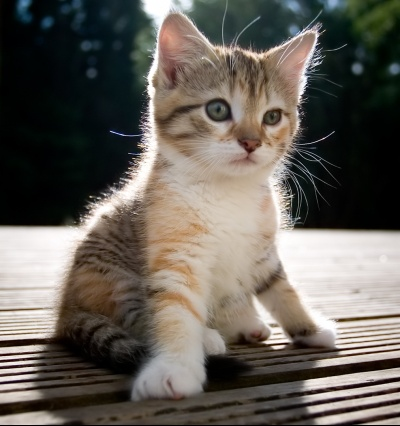
\includegraphics[scale=0.8]{images/chat.jpg}
\caption{L'image de départ}
\label{chat1}
\end{figure}

\begin{figure}[!h]
\centering
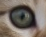
\includegraphics[scale=2]{images/chat_orig.jpg}
\caption{Détail de l'image de départ}
\label{dchat}
\end{figure}

La figure \ref{chat2} représente le même détail de l'image une fois que la compression a été appliquée avec un seuil assez petit pour garder la plupart des détails importants de l'image mais assez grand pour compresser les <<aplats>> de couleur, les ombres, etc. L'image compressée occupe 35\% de mémoire en moins par rapport à l'image de départ. Ce qui montre que la compression par ondelettes est plutôt efficace et que notre algorithme est fonctionnel.

\begin{figure}[!h]
\centering
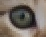
\includegraphics[scale=2]{images/chat_compress.jpg}
\caption{Détail de l'image compressée}
\label{chat2}
\end{figure}

Sur la figure \ref{chat3}, on peut voir le même détail quand l'image a été compressée avec le seuil maximal. Ici, tous les détails ont été éliminés. Cela revient simplement à diviser la résolution de l'image par deux.

\begin{figure}[!h]
\centering
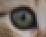
\includegraphics[scale=2]{images/chat_compress255.jpg}
\caption{Détail de l'image compressée à 100\%}
\label{chat3}
\end{figure}

\cleardoublepage

\subsection{L'application graphique}

L'application graphique que nous avons créée permet plusieurs choses :

\begin{itemize}
\item Ouverture d'une image
\item Enregistrement d'une image
\item Affichage d'une image dans une fenêtre
\item Conversion d'une image en nuances de gris
\item Compression d'une image par deux méthodes
\item Réduction de la résolution d'une image de 50\%
\item Envoi d'une image à un serveur grâce au programme @client.py@
\end{itemize}

La figure \ref{GUI} montre la fenêtre principale de l'application, avec une image en cours d'édition. L'interface est minimaliste, mais suffisante.


\begin{figure}[!hb]
\centering
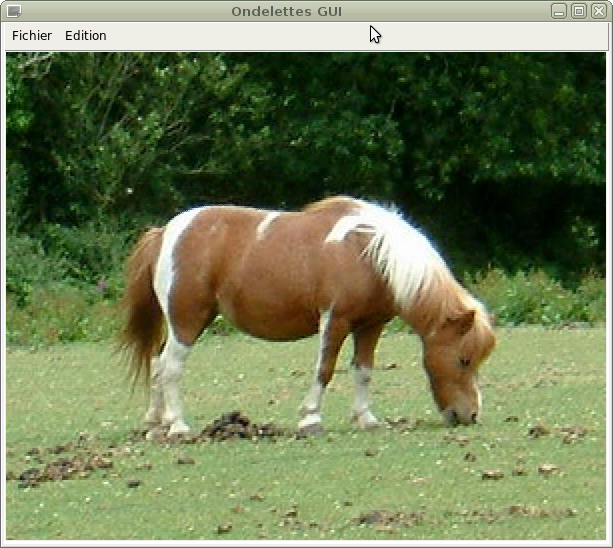
\includegraphics[scale=0.5]{images/OndelettesGUI.png}
\caption{Fenêtre principale de l'application}
\label{GUI}
\end{figure}


La figure \ref{GUI1} montre les menus de l'application, qui permettent de choisir entre toutes les actions décrites ci-dessus.

\begin{figure}[!ht]
\centering
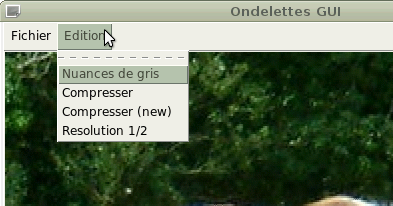
\includegraphics[scale=0.8]{images/OndelettesGUI1.png}
\caption{Menus de l'application}
\label{GUI1}
\end{figure}

La figure \ref{GUI2} montre le sélecteur de seuil, qui apparaît lorsqu'on choisit <<Compresser>> ou <<Compresser (new)>> dans les menus.

\begin{figure}[!hb]
\centering
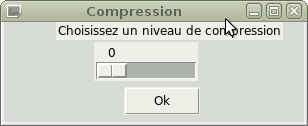
\includegraphics[scale=0.8]{images/Compression.png}
\caption{Le sélecteur de seuil de compression}
\label{GUI2}
\end{figure}



\cleardoublepage

\subsection{L'algorithme fasthaar}

Nous avons mis au point un autre algorithme de compression n'utilisant pas de matrices. Celui-ci est plus rapide et moins gourmand en mémoire que @haar@, mais l'inconvénient est qu'il ne permet pas d'utiliser la transformation par ondelettes discrète à un niveau de récursivité plus grand que 1.

\subsubsection{Fonctionnement}

L'algorithme découpe l'image en carrés de 4 pixels, qu'il va traiter à la suite, colonne par colonne. Comme montré sur la figure \ref{algo}

\begin{figure}[!h]
\centering
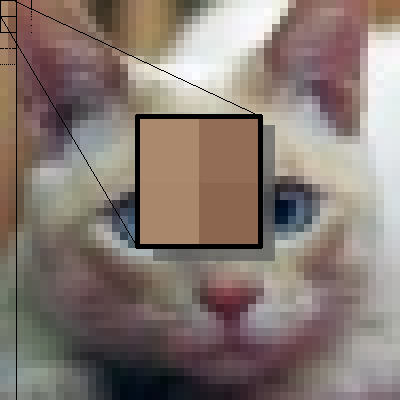
\includegraphics[scale=0.8]{images/minichat.jpg}
\caption{Fonctionnement de l'algorithme}
\label{algo}
\end{figure}

\paragraph{Analyse :}

Pour chaque carré de 4 pixels, l'algorithme applique la transformation par ondelettes discrète. On commence par stocker les valeurs RGB des 4 pixels dans un tableau. Nous allons, pour l'exemple, utiliser les 4 pixels mis en valeur sur la figure \ref{algo}. Le tableau créé est montré par la figure \ref{tab1}.

\begin{figure}[!h]
\begin{center}
\begin{tabular}{|c|c|c|c|c|c|}
\hline
\multicolumn{2}{|c|}{R} & \multicolumn{2}{|c|}{G}  & \multicolumn{2}{|c|}{B} \\
\hline
171    & 147   &   137  & 109 &   109  & 86   \\ 
\hline
169    & 140   &   135  & 102 &   107  & 79 \\
\hline
\end{tabular}
\end{center}
\caption{Tableau créé par l'algorithme}
\label{tab1}
\end{figure}


L'algorithme remplace ensuite les valeurs des colonnes de gauche de chaque couleur par la moyenne  de chaque ligne et les valeurs des colonnes de droite par la différence divisée par deux. Ce qui nous donne le tableau de la figure \ref{tab2}. Les coefficients d'ondelette sont surlignés.

\begin{figure}[!h]
\begin{center}
\begin{tabular}{|c|c|c|c|c|c|}
\hline
\multicolumn{2}{|c|}{R} & \multicolumn{2}{|c|}{G}  & \multicolumn{2}{|c|}{B} \\
\hline
160    & \hl{11}   &   123  & \hl{14} &   97.5  & \hl{11.5}   \\ 
\hline
154.5    & \hl{14.5}   &   118.5  & \hl{16.5} &   93  & \hl{14} \\
\hline
\end{tabular}
\end{center}
\caption{Tableau après l'étape 1}
\label{tab2}
\end{figure}


Enfin, l'algorithme remplace la case en haut à gauche de chaque couleur par la moyenne des lignes et la case en bas à gauche par la différence divisée par deux. Le résultat est montré par la figure \ref{tab3}.

\begin{figure}[!h]
\begin{center}
\begin{tabular}{|c|c|c|c|c|c|}
\hline
\multicolumn{2}{|c|}{R} & \multicolumn{2}{|c|}{G}  & \multicolumn{2}{|c|}{B} \\
\hline
157.25    & \hl{11}   &   120.75  & \hl{14} &   95.25  & \hl{11.5}   \\ 
\hline
\hl{2.75}    & \hl{14.5}   &   \hl{2.25}  & \hl{16.5} &   \hl{2.25}  & \hl{14} \\
\hline
\end{tabular}
\end{center}
\caption{Tableau après l'étape 2}
\label{tab3}
\end{figure}



\paragraph{Compression et synthèse :}

Après la phase d'analyse vient la phase de compression. On va supprimer les coefficients d'ondelettes inférieurs à un certain seuil. Pour l'exemple, nous allons choisir un seuil de 12.

Après compression, le tableau est celui de la figure \ref{tab4}.

\begin{figure}[!h]
\begin{center}
\begin{tabular}{|c|c|c|c|c|c|}
\hline
\multicolumn{2}{|c|}{R} & \multicolumn{2}{|c|}{G}  & \multicolumn{2}{|c|}{B} \\
\hline
157.25    & \hl{0}   &   120.75  & \hl{14} &   95.25  & \hl{0}   \\ 
\hline
\hl{0}    & \hl{14.5}   &   \hl{0}  & \hl{16.5} &   \hl{0}  & \hl{14} \\
\hline
\end{tabular}
\end{center}
\caption{Tableau après compression}
\label{tab4}
\end{figure}

Ensuite, l'algorithme reconstitue l'image avec les coefficients restants. On effectue d'abord pour la colonne de gauche de chaque couleur une addition pour retrouver le coefficient du haut, et une soustraction pour le coefficient du bas. Ce qui nous donne le tableau de la figure \ref{tab5}. Puisque les coefficients étaient égaux à 0, les pixels ne sont pas changés.

\begin{figure}[!h]
\begin{center}
\begin{tabular}{|c|c|c|c|c|c|}
\hline
\multicolumn{2}{|c|}{R} & \multicolumn{2}{|c|}{G}  & \multicolumn{2}{|c|}{B} \\
\hline
157.25    & \hl{0}   &   120.75  & \hl{14} &   95.25  & \hl{0}   \\ 
\hline
157.25    & \hl{14.5}   &   120.75  & \hl{16.5} &   95.25  & \hl{14} \\
\hline
\end{tabular}
\end{center}
\caption{Tableau après synthèse sur les colonnes}
\label{tab5}
\end{figure}

L'algorithme effectue ensuite les mêmes opérations sur les lignes. Le résultat est donné par la figure  \ref{tab6}

\begin{figure}[!h]
\begin{center}
\begin{tabular}{|c|c|c|c|c|c|}
\hline
\multicolumn{2}{|c|}{R} & \multicolumn{2}{|c|}{G}  & \multicolumn{2}{|c|}{B} \\
\hline
157.25    & 157.25   &   134.75  & 106.75 &   95.25  & 95.25   \\ 
\hline
171.75    & 143   &   137.25  & 104.25 &   109.25  & 81.25 \\
\hline
\end{tabular}
\end{center}
\caption{Tableau après synthèse sur les lignes}
\label{tab6}
\end{figure}

Enfin, on arrondit les valeurs à l'entier le plus proche. Le tableau final est donné par la figure \ref{tab7}. La figure \ref{after} montre une comparaison entre l'état des pixels avant traitement, et l'état des pixels après.

\begin{figure}[!h]
\begin{center}
\begin{tabular}{|c|c|c|c|c|c|}
\hline
\multicolumn{2}{|c|}{R} & \multicolumn{2}{|c|}{G}  & \multicolumn{2}{|c|}{B} \\
\hline
157    & 157  &   135  & 107 &   95  & 95   \\ 
\hline
172   & 143   &   137  & 104 &   109  & 81 \\
\hline
\end{tabular}
\end{center}
\caption{Tableau après synthèse sur les lignes}
\label{tab7}
\end{figure}

\begin{figure}[!h]
\centering
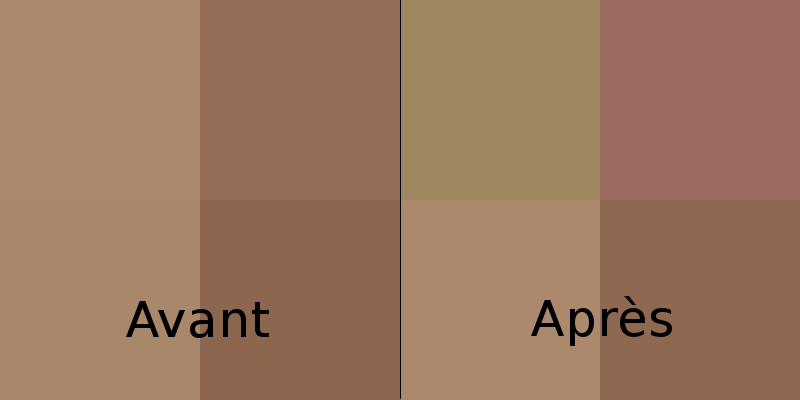
\includegraphics[scale=0.3]{images/aprescompress.jpg}
\caption{Pixels avant et après traitement}
\label{after}
\end{figure}

Les pixels peuvent sembler réellement différents après traitement, mais la valeur moyenne des couleurs est conservée, ce qui, au final, donnera le même rendu quand les pixels seront à leur taille normale.

\clearpage

\subsubsection{Coût et Performance}

Nous avons été curieux de voir les performances de l'algorithme @fasthaar@.

\paragraph{Coût en mémoire :}

Cet algorithme est peu coûteux en mémoire, par rapport à la version matricielle. En effet, ce dernier devait stocker plusieurs matrices contenant l'image, les coefficients d'ondelettes, les différentes couleurs, etc. @fasthaar@, quant à lui, ne stocke que l'image et les valeurs de 4 pixels. Un pixel est un tuple contenant 3 entiers codés sur 8 bits (= 1 octet). 

Soient $L$ et $l$ la longueur et la largeur de l'image à traiter. 
La place de l'algorithme @fasthaar@ en mémoire est donc de $3\times{}l\times{}L + 4 \times{} 3$ octets.

\paragraph{Coût temporel :}

Vu le principe de fonctionnement de @fasthaar@, on peut deviner que celui-ci a un coût en $O(l\cdot L)$ (ou $O(n^2)$ pour une image carrée de côté $n$). Nous avons créé un fichier @bench.py@ servant à mesurer le temps que prend l'algorithme à traiter des images de différentes tailles. L'algorithme génère une image d'une taille donnée avec des pixels aléatoires puis lui applique @fasthaar@ en chronométrant. 

La figure \ref{bench1} représente le temps de traitement d'une image (en secondes) en fonction de sa taille (pixels d'un côté divisé par 2). On vérifie donc que le coût est bien quadratique. 

\begin{figure}[!h]
\begin{center}
% GNUPLOT: LaTeX picture
\setlength{\unitlength}{0.240900pt}
\ifx\plotpoint\undefined\newsavebox{\plotpoint}\fi
\sbox{\plotpoint}{\rule[-0.200pt]{0.400pt}{0.400pt}}%
\begin{picture}(1500,900)(0,0)
\sbox{\plotpoint}{\rule[-0.200pt]{0.400pt}{0.400pt}}%
\put(151.0,131.0){\rule[-0.200pt]{4.818pt}{0.400pt}}
\put(131,131){\makebox(0,0)[r]{ 0}}
\put(1419.0,131.0){\rule[-0.200pt]{4.818pt}{0.400pt}}
\put(151.0,235.0){\rule[-0.200pt]{4.818pt}{0.400pt}}
\put(131,235){\makebox(0,0)[r]{ 5}}
\put(1419.0,235.0){\rule[-0.200pt]{4.818pt}{0.400pt}}
\put(151.0,339.0){\rule[-0.200pt]{4.818pt}{0.400pt}}
\put(131,339){\makebox(0,0)[r]{ 10}}
\put(1419.0,339.0){\rule[-0.200pt]{4.818pt}{0.400pt}}
\put(151.0,443.0){\rule[-0.200pt]{4.818pt}{0.400pt}}
\put(131,443){\makebox(0,0)[r]{ 15}}
\put(1419.0,443.0){\rule[-0.200pt]{4.818pt}{0.400pt}}
\put(151.0,547.0){\rule[-0.200pt]{4.818pt}{0.400pt}}
\put(131,547){\makebox(0,0)[r]{ 20}}
\put(1419.0,547.0){\rule[-0.200pt]{4.818pt}{0.400pt}}
\put(151.0,651.0){\rule[-0.200pt]{4.818pt}{0.400pt}}
\put(131,651){\makebox(0,0)[r]{ 25}}
\put(1419.0,651.0){\rule[-0.200pt]{4.818pt}{0.400pt}}
\put(151.0,755.0){\rule[-0.200pt]{4.818pt}{0.400pt}}
\put(131,755){\makebox(0,0)[r]{ 30}}
\put(1419.0,755.0){\rule[-0.200pt]{4.818pt}{0.400pt}}
\put(151.0,859.0){\rule[-0.200pt]{4.818pt}{0.400pt}}
\put(131,859){\makebox(0,0)[r]{ 35}}
\put(1419.0,859.0){\rule[-0.200pt]{4.818pt}{0.400pt}}
\put(151.0,131.0){\rule[-0.200pt]{0.400pt}{4.818pt}}
\put(151,90){\makebox(0,0){ 0}}
\put(151.0,839.0){\rule[-0.200pt]{0.400pt}{4.818pt}}
\put(280.0,131.0){\rule[-0.200pt]{0.400pt}{4.818pt}}
\put(280,90){\makebox(0,0){ 100}}
\put(280.0,839.0){\rule[-0.200pt]{0.400pt}{4.818pt}}
\put(409.0,131.0){\rule[-0.200pt]{0.400pt}{4.818pt}}
\put(409,90){\makebox(0,0){ 200}}
\put(409.0,839.0){\rule[-0.200pt]{0.400pt}{4.818pt}}
\put(537.0,131.0){\rule[-0.200pt]{0.400pt}{4.818pt}}
\put(537,90){\makebox(0,0){ 300}}
\put(537.0,839.0){\rule[-0.200pt]{0.400pt}{4.818pt}}
\put(666.0,131.0){\rule[-0.200pt]{0.400pt}{4.818pt}}
\put(666,90){\makebox(0,0){ 400}}
\put(666.0,839.0){\rule[-0.200pt]{0.400pt}{4.818pt}}
\put(795.0,131.0){\rule[-0.200pt]{0.400pt}{4.818pt}}
\put(795,90){\makebox(0,0){ 500}}
\put(795.0,839.0){\rule[-0.200pt]{0.400pt}{4.818pt}}
\put(924.0,131.0){\rule[-0.200pt]{0.400pt}{4.818pt}}
\put(924,90){\makebox(0,0){ 600}}
\put(924.0,839.0){\rule[-0.200pt]{0.400pt}{4.818pt}}
\put(1053.0,131.0){\rule[-0.200pt]{0.400pt}{4.818pt}}
\put(1053,90){\makebox(0,0){ 700}}
\put(1053.0,839.0){\rule[-0.200pt]{0.400pt}{4.818pt}}
\put(1181.0,131.0){\rule[-0.200pt]{0.400pt}{4.818pt}}
\put(1181,90){\makebox(0,0){ 800}}
\put(1181.0,839.0){\rule[-0.200pt]{0.400pt}{4.818pt}}
\put(1310.0,131.0){\rule[-0.200pt]{0.400pt}{4.818pt}}
\put(1310,90){\makebox(0,0){ 900}}
\put(1310.0,839.0){\rule[-0.200pt]{0.400pt}{4.818pt}}
\put(1439.0,131.0){\rule[-0.200pt]{0.400pt}{4.818pt}}
\put(1439,90){\makebox(0,0){ 1000}}
\put(1439.0,839.0){\rule[-0.200pt]{0.400pt}{4.818pt}}
\put(151.0,131.0){\rule[-0.200pt]{0.400pt}{175.375pt}}
\put(151.0,131.0){\rule[-0.200pt]{310.279pt}{0.400pt}}
\put(1439.0,131.0){\rule[-0.200pt]{0.400pt}{175.375pt}}
\put(151.0,859.0){\rule[-0.200pt]{310.279pt}{0.400pt}}
\put(30,495){\makebox(0,0){\rotatebox{90}{Temps de compression (s)}}}
\put(795,29){\makebox(0,0){Taille de l'image (px/2)}}
\put(152,131){\usebox{\plotpoint}}
\put(184,130.67){\rule{0.482pt}{0.400pt}}
\multiput(184.00,130.17)(1.000,1.000){2}{\rule{0.241pt}{0.400pt}}
\put(152.0,131.0){\rule[-0.200pt]{7.709pt}{0.400pt}}
\put(210,131.67){\rule{0.482pt}{0.400pt}}
\multiput(210.00,131.17)(1.000,1.000){2}{\rule{0.241pt}{0.400pt}}
\put(186.0,132.0){\rule[-0.200pt]{5.782pt}{0.400pt}}
\put(227,132.67){\rule{0.241pt}{0.400pt}}
\multiput(227.00,132.17)(0.500,1.000){2}{\rule{0.120pt}{0.400pt}}
\put(212.0,133.0){\rule[-0.200pt]{3.613pt}{0.400pt}}
\put(240,133.67){\rule{0.241pt}{0.400pt}}
\multiput(240.00,133.17)(0.500,1.000){2}{\rule{0.120pt}{0.400pt}}
\put(228.0,134.0){\rule[-0.200pt]{2.891pt}{0.400pt}}
\put(255,134.67){\rule{0.482pt}{0.400pt}}
\multiput(255.00,134.17)(1.000,1.000){2}{\rule{0.241pt}{0.400pt}}
\put(241.0,135.0){\rule[-0.200pt]{3.373pt}{0.400pt}}
\put(267,135.67){\rule{0.241pt}{0.400pt}}
\multiput(267.00,135.17)(0.500,1.000){2}{\rule{0.120pt}{0.400pt}}
\put(257.0,136.0){\rule[-0.200pt]{2.409pt}{0.400pt}}
\put(277,136.67){\rule{0.482pt}{0.400pt}}
\multiput(277.00,136.17)(1.000,1.000){2}{\rule{0.241pt}{0.400pt}}
\put(268.0,137.0){\rule[-0.200pt]{2.168pt}{0.400pt}}
\put(285,137.67){\rule{0.241pt}{0.400pt}}
\multiput(285.00,137.17)(0.500,1.000){2}{\rule{0.120pt}{0.400pt}}
\put(279.0,138.0){\rule[-0.200pt]{1.445pt}{0.400pt}}
\put(289,138.67){\rule{0.241pt}{0.400pt}}
\multiput(289.00,138.17)(0.500,1.000){2}{\rule{0.120pt}{0.400pt}}
\put(286.0,139.0){\rule[-0.200pt]{0.723pt}{0.400pt}}
\put(291,138.67){\rule{0.482pt}{0.400pt}}
\multiput(291.00,139.17)(1.000,-1.000){2}{\rule{0.241pt}{0.400pt}}
\put(293,138.67){\rule{0.241pt}{0.400pt}}
\multiput(293.00,138.17)(0.500,1.000){2}{\rule{0.120pt}{0.400pt}}
\put(290.0,140.0){\usebox{\plotpoint}}
\put(303,139.67){\rule{0.241pt}{0.400pt}}
\multiput(303.00,139.17)(0.500,1.000){2}{\rule{0.120pt}{0.400pt}}
\put(294.0,140.0){\rule[-0.200pt]{2.168pt}{0.400pt}}
\put(309,140.67){\rule{0.482pt}{0.400pt}}
\multiput(309.00,140.17)(1.000,1.000){2}{\rule{0.241pt}{0.400pt}}
\put(304.0,141.0){\rule[-0.200pt]{1.204pt}{0.400pt}}
\put(317,141.67){\rule{0.241pt}{0.400pt}}
\multiput(317.00,141.17)(0.500,1.000){2}{\rule{0.120pt}{0.400pt}}
\put(311.0,142.0){\rule[-0.200pt]{1.445pt}{0.400pt}}
\put(321,142.67){\rule{0.241pt}{0.400pt}}
\multiput(321.00,142.17)(0.500,1.000){2}{\rule{0.120pt}{0.400pt}}
\put(322,142.67){\rule{0.482pt}{0.400pt}}
\multiput(322.00,143.17)(1.000,-1.000){2}{\rule{0.241pt}{0.400pt}}
\put(324,142.67){\rule{0.241pt}{0.400pt}}
\multiput(324.00,142.17)(0.500,1.000){2}{\rule{0.120pt}{0.400pt}}
\put(318.0,143.0){\rule[-0.200pt]{0.723pt}{0.400pt}}
\put(330,143.67){\rule{0.241pt}{0.400pt}}
\multiput(330.00,143.17)(0.500,1.000){2}{\rule{0.120pt}{0.400pt}}
\put(325.0,144.0){\rule[-0.200pt]{1.204pt}{0.400pt}}
\put(334,144.67){\rule{0.241pt}{0.400pt}}
\multiput(334.00,144.17)(0.500,1.000){2}{\rule{0.120pt}{0.400pt}}
\put(335,144.67){\rule{0.241pt}{0.400pt}}
\multiput(335.00,145.17)(0.500,-1.000){2}{\rule{0.120pt}{0.400pt}}
\put(336,144.67){\rule{0.482pt}{0.400pt}}
\multiput(336.00,144.17)(1.000,1.000){2}{\rule{0.241pt}{0.400pt}}
\put(331.0,145.0){\rule[-0.200pt]{0.723pt}{0.400pt}}
\put(340,145.67){\rule{0.482pt}{0.400pt}}
\multiput(340.00,145.17)(1.000,1.000){2}{\rule{0.241pt}{0.400pt}}
\put(338.0,146.0){\rule[-0.200pt]{0.482pt}{0.400pt}}
\put(348,146.67){\rule{0.241pt}{0.400pt}}
\multiput(348.00,146.17)(0.500,1.000){2}{\rule{0.120pt}{0.400pt}}
\put(349,146.67){\rule{0.482pt}{0.400pt}}
\multiput(349.00,147.17)(1.000,-1.000){2}{\rule{0.241pt}{0.400pt}}
\put(351,146.67){\rule{0.241pt}{0.400pt}}
\multiput(351.00,146.17)(0.500,1.000){2}{\rule{0.120pt}{0.400pt}}
\put(342.0,147.0){\rule[-0.200pt]{1.445pt}{0.400pt}}
\put(355,147.67){\rule{0.241pt}{0.400pt}}
\multiput(355.00,147.17)(0.500,1.000){2}{\rule{0.120pt}{0.400pt}}
\put(352.0,148.0){\rule[-0.200pt]{0.723pt}{0.400pt}}
\put(362,148.67){\rule{0.482pt}{0.400pt}}
\multiput(362.00,148.17)(1.000,1.000){2}{\rule{0.241pt}{0.400pt}}
\put(364,149.67){\rule{0.241pt}{0.400pt}}
\multiput(364.00,149.17)(0.500,1.000){2}{\rule{0.120pt}{0.400pt}}
\put(356.0,149.0){\rule[-0.200pt]{1.445pt}{0.400pt}}
\put(367,149.67){\rule{0.482pt}{0.400pt}}
\multiput(367.00,150.17)(1.000,-1.000){2}{\rule{0.241pt}{0.400pt}}
\put(369,149.67){\rule{0.241pt}{0.400pt}}
\multiput(369.00,149.17)(0.500,1.000){2}{\rule{0.120pt}{0.400pt}}
\put(365.0,151.0){\rule[-0.200pt]{0.482pt}{0.400pt}}
\put(371,150.67){\rule{0.482pt}{0.400pt}}
\multiput(371.00,150.17)(1.000,1.000){2}{\rule{0.241pt}{0.400pt}}
\put(370.0,151.0){\usebox{\plotpoint}}
\put(374,150.67){\rule{0.241pt}{0.400pt}}
\multiput(374.00,151.17)(0.500,-1.000){2}{\rule{0.120pt}{0.400pt}}
\put(375,150.67){\rule{0.241pt}{0.400pt}}
\multiput(375.00,150.17)(0.500,1.000){2}{\rule{0.120pt}{0.400pt}}
\put(376,151.67){\rule{0.482pt}{0.400pt}}
\multiput(376.00,151.17)(1.000,1.000){2}{\rule{0.241pt}{0.400pt}}
\put(373.0,152.0){\usebox{\plotpoint}}
\put(382,152.67){\rule{0.241pt}{0.400pt}}
\multiput(382.00,152.17)(0.500,1.000){2}{\rule{0.120pt}{0.400pt}}
\put(378.0,153.0){\rule[-0.200pt]{0.964pt}{0.400pt}}
\put(387,153.67){\rule{0.241pt}{0.400pt}}
\multiput(387.00,153.17)(0.500,1.000){2}{\rule{0.120pt}{0.400pt}}
\put(383.0,154.0){\rule[-0.200pt]{0.964pt}{0.400pt}}
\put(392,154.67){\rule{0.241pt}{0.400pt}}
\multiput(392.00,154.17)(0.500,1.000){2}{\rule{0.120pt}{0.400pt}}
\put(388.0,155.0){\rule[-0.200pt]{0.964pt}{0.400pt}}
\put(398,155.67){\rule{0.482pt}{0.400pt}}
\multiput(398.00,155.17)(1.000,1.000){2}{\rule{0.241pt}{0.400pt}}
\put(400,156.67){\rule{0.241pt}{0.400pt}}
\multiput(400.00,156.17)(0.500,1.000){2}{\rule{0.120pt}{0.400pt}}
\put(393.0,156.0){\rule[-0.200pt]{1.204pt}{0.400pt}}
\put(405,157.67){\rule{0.241pt}{0.400pt}}
\multiput(405.00,157.17)(0.500,1.000){2}{\rule{0.120pt}{0.400pt}}
\put(401.0,158.0){\rule[-0.200pt]{0.964pt}{0.400pt}}
\put(407,158.67){\rule{0.482pt}{0.400pt}}
\multiput(407.00,158.17)(1.000,1.000){2}{\rule{0.241pt}{0.400pt}}
\put(409,158.67){\rule{0.241pt}{0.400pt}}
\multiput(409.00,159.17)(0.500,-1.000){2}{\rule{0.120pt}{0.400pt}}
\put(406.0,159.0){\usebox{\plotpoint}}
\put(411,158.67){\rule{0.241pt}{0.400pt}}
\multiput(411.00,158.17)(0.500,1.000){2}{\rule{0.120pt}{0.400pt}}
\put(410.0,159.0){\usebox{\plotpoint}}
\put(414,159.67){\rule{0.241pt}{0.400pt}}
\multiput(414.00,159.17)(0.500,1.000){2}{\rule{0.120pt}{0.400pt}}
\put(412.0,160.0){\rule[-0.200pt]{0.482pt}{0.400pt}}
\put(416,160.67){\rule{0.482pt}{0.400pt}}
\multiput(416.00,160.17)(1.000,1.000){2}{\rule{0.241pt}{0.400pt}}
\put(415.0,161.0){\usebox{\plotpoint}}
\put(420,160.67){\rule{0.241pt}{0.400pt}}
\multiput(420.00,161.17)(0.500,-1.000){2}{\rule{0.120pt}{0.400pt}}
\put(421,161.17){\rule{0.482pt}{0.400pt}}
\multiput(421.00,160.17)(1.000,2.000){2}{\rule{0.241pt}{0.400pt}}
\put(418.0,162.0){\rule[-0.200pt]{0.482pt}{0.400pt}}
\put(424,161.67){\rule{0.241pt}{0.400pt}}
\multiput(424.00,162.17)(0.500,-1.000){2}{\rule{0.120pt}{0.400pt}}
\put(425,162.17){\rule{0.482pt}{0.400pt}}
\multiput(425.00,161.17)(1.000,2.000){2}{\rule{0.241pt}{0.400pt}}
\put(426.67,162){\rule{0.400pt}{0.482pt}}
\multiput(426.17,163.00)(1.000,-1.000){2}{\rule{0.400pt}{0.241pt}}
\put(428,161.67){\rule{0.241pt}{0.400pt}}
\multiput(428.00,161.17)(0.500,1.000){2}{\rule{0.120pt}{0.400pt}}
\put(429,162.67){\rule{0.241pt}{0.400pt}}
\multiput(429.00,162.17)(0.500,1.000){2}{\rule{0.120pt}{0.400pt}}
\put(430,163.67){\rule{0.482pt}{0.400pt}}
\multiput(430.00,163.17)(1.000,1.000){2}{\rule{0.241pt}{0.400pt}}
\put(432,164.67){\rule{0.241pt}{0.400pt}}
\multiput(432.00,164.17)(0.500,1.000){2}{\rule{0.120pt}{0.400pt}}
\put(423.0,163.0){\usebox{\plotpoint}}
\put(441,165.67){\rule{0.241pt}{0.400pt}}
\multiput(441.00,165.17)(0.500,1.000){2}{\rule{0.120pt}{0.400pt}}
\put(433.0,166.0){\rule[-0.200pt]{1.927pt}{0.400pt}}
\put(443,166.67){\rule{0.482pt}{0.400pt}}
\multiput(443.00,166.17)(1.000,1.000){2}{\rule{0.241pt}{0.400pt}}
\put(442.0,167.0){\usebox{\plotpoint}}
\put(446,167.67){\rule{0.241pt}{0.400pt}}
\multiput(446.00,167.17)(0.500,1.000){2}{\rule{0.120pt}{0.400pt}}
\put(445.0,168.0){\usebox{\plotpoint}}
\put(450,168.67){\rule{0.241pt}{0.400pt}}
\multiput(450.00,168.17)(0.500,1.000){2}{\rule{0.120pt}{0.400pt}}
\put(447.0,169.0){\rule[-0.200pt]{0.723pt}{0.400pt}}
\put(454,169.67){\rule{0.241pt}{0.400pt}}
\multiput(454.00,169.17)(0.500,1.000){2}{\rule{0.120pt}{0.400pt}}
\put(455,169.67){\rule{0.241pt}{0.400pt}}
\multiput(455.00,170.17)(0.500,-1.000){2}{\rule{0.120pt}{0.400pt}}
\put(456,169.67){\rule{0.482pt}{0.400pt}}
\multiput(456.00,169.17)(1.000,1.000){2}{\rule{0.241pt}{0.400pt}}
\put(451.0,170.0){\rule[-0.200pt]{0.723pt}{0.400pt}}
\put(459,170.67){\rule{0.241pt}{0.400pt}}
\multiput(459.00,170.17)(0.500,1.000){2}{\rule{0.120pt}{0.400pt}}
\put(460,170.67){\rule{0.241pt}{0.400pt}}
\multiput(460.00,171.17)(0.500,-1.000){2}{\rule{0.120pt}{0.400pt}}
\put(461,171.17){\rule{0.482pt}{0.400pt}}
\multiput(461.00,170.17)(1.000,2.000){2}{\rule{0.241pt}{0.400pt}}
\put(458.0,171.0){\usebox{\plotpoint}}
\put(465,172.67){\rule{0.482pt}{0.400pt}}
\multiput(465.00,172.17)(1.000,1.000){2}{\rule{0.241pt}{0.400pt}}
\put(467,172.67){\rule{0.241pt}{0.400pt}}
\multiput(467.00,173.17)(0.500,-1.000){2}{\rule{0.120pt}{0.400pt}}
\put(463.0,173.0){\rule[-0.200pt]{0.482pt}{0.400pt}}
\put(468.67,173){\rule{0.400pt}{0.482pt}}
\multiput(468.17,173.00)(1.000,1.000){2}{\rule{0.400pt}{0.241pt}}
\put(468.0,173.0){\usebox{\plotpoint}}
\put(472,173.67){\rule{0.241pt}{0.400pt}}
\multiput(472.00,174.17)(0.500,-1.000){2}{\rule{0.120pt}{0.400pt}}
\put(473,173.67){\rule{0.241pt}{0.400pt}}
\multiput(473.00,173.17)(0.500,1.000){2}{\rule{0.120pt}{0.400pt}}
\put(470.0,175.0){\rule[-0.200pt]{0.482pt}{0.400pt}}
\put(475.67,175){\rule{0.400pt}{0.482pt}}
\multiput(475.17,175.00)(1.000,1.000){2}{\rule{0.400pt}{0.241pt}}
\put(474.0,175.0){\rule[-0.200pt]{0.482pt}{0.400pt}}
\put(478,176.67){\rule{0.241pt}{0.400pt}}
\multiput(478.00,176.17)(0.500,1.000){2}{\rule{0.120pt}{0.400pt}}
\put(479,176.67){\rule{0.482pt}{0.400pt}}
\multiput(479.00,177.17)(1.000,-1.000){2}{\rule{0.241pt}{0.400pt}}
\put(477.0,177.0){\usebox{\plotpoint}}
\put(483,176.67){\rule{0.482pt}{0.400pt}}
\multiput(483.00,176.17)(1.000,1.000){2}{\rule{0.241pt}{0.400pt}}
\put(481.0,177.0){\rule[-0.200pt]{0.482pt}{0.400pt}}
\put(486,177.67){\rule{0.241pt}{0.400pt}}
\multiput(486.00,177.17)(0.500,1.000){2}{\rule{0.120pt}{0.400pt}}
\put(487,178.67){\rule{0.241pt}{0.400pt}}
\multiput(487.00,178.17)(0.500,1.000){2}{\rule{0.120pt}{0.400pt}}
\put(488,178.67){\rule{0.482pt}{0.400pt}}
\multiput(488.00,179.17)(1.000,-1.000){2}{\rule{0.241pt}{0.400pt}}
\put(490,178.67){\rule{0.241pt}{0.400pt}}
\multiput(490.00,178.17)(0.500,1.000){2}{\rule{0.120pt}{0.400pt}}
\put(485.0,178.0){\usebox{\plotpoint}}
\put(492,179.67){\rule{0.482pt}{0.400pt}}
\multiput(492.00,179.17)(1.000,1.000){2}{\rule{0.241pt}{0.400pt}}
\put(494,180.67){\rule{0.241pt}{0.400pt}}
\multiput(494.00,180.17)(0.500,1.000){2}{\rule{0.120pt}{0.400pt}}
\put(495,180.67){\rule{0.241pt}{0.400pt}}
\multiput(495.00,181.17)(0.500,-1.000){2}{\rule{0.120pt}{0.400pt}}
\put(496,180.67){\rule{0.241pt}{0.400pt}}
\multiput(496.00,180.17)(0.500,1.000){2}{\rule{0.120pt}{0.400pt}}
\put(491.0,180.0){\usebox{\plotpoint}}
\put(499,181.67){\rule{0.241pt}{0.400pt}}
\multiput(499.00,181.17)(0.500,1.000){2}{\rule{0.120pt}{0.400pt}}
\put(500,182.67){\rule{0.241pt}{0.400pt}}
\multiput(500.00,182.17)(0.500,1.000){2}{\rule{0.120pt}{0.400pt}}
\put(497.0,182.0){\rule[-0.200pt]{0.482pt}{0.400pt}}
\put(503,183.67){\rule{0.241pt}{0.400pt}}
\multiput(503.00,183.17)(0.500,1.000){2}{\rule{0.120pt}{0.400pt}}
\put(504,183.67){\rule{0.241pt}{0.400pt}}
\multiput(504.00,184.17)(0.500,-1.000){2}{\rule{0.120pt}{0.400pt}}
\put(501.0,184.0){\rule[-0.200pt]{0.482pt}{0.400pt}}
\put(506,184.17){\rule{0.482pt}{0.400pt}}
\multiput(506.00,183.17)(1.000,2.000){2}{\rule{0.241pt}{0.400pt}}
\put(508,184.67){\rule{0.241pt}{0.400pt}}
\multiput(508.00,185.17)(0.500,-1.000){2}{\rule{0.120pt}{0.400pt}}
\put(509,184.67){\rule{0.241pt}{0.400pt}}
\multiput(509.00,184.17)(0.500,1.000){2}{\rule{0.120pt}{0.400pt}}
\put(510,185.67){\rule{0.482pt}{0.400pt}}
\multiput(510.00,185.17)(1.000,1.000){2}{\rule{0.241pt}{0.400pt}}
\put(505.0,184.0){\usebox{\plotpoint}}
\put(513,186.67){\rule{0.241pt}{0.400pt}}
\multiput(513.00,186.17)(0.500,1.000){2}{\rule{0.120pt}{0.400pt}}
\put(512.0,187.0){\usebox{\plotpoint}}
\put(516.67,188){\rule{0.400pt}{0.482pt}}
\multiput(516.17,188.00)(1.000,1.000){2}{\rule{0.400pt}{0.241pt}}
\put(517.67,188){\rule{0.400pt}{0.482pt}}
\multiput(517.17,189.00)(1.000,-1.000){2}{\rule{0.400pt}{0.241pt}}
\put(519,187.67){\rule{0.482pt}{0.400pt}}
\multiput(519.00,187.17)(1.000,1.000){2}{\rule{0.241pt}{0.400pt}}
\put(521,188.67){\rule{0.241pt}{0.400pt}}
\multiput(521.00,188.17)(0.500,1.000){2}{\rule{0.120pt}{0.400pt}}
\put(522,188.67){\rule{0.241pt}{0.400pt}}
\multiput(522.00,189.17)(0.500,-1.000){2}{\rule{0.120pt}{0.400pt}}
\put(514.0,188.0){\rule[-0.200pt]{0.723pt}{0.400pt}}
\put(525,188.67){\rule{0.241pt}{0.400pt}}
\multiput(525.00,188.17)(0.500,1.000){2}{\rule{0.120pt}{0.400pt}}
\put(526,188.67){\rule{0.241pt}{0.400pt}}
\multiput(526.00,189.17)(0.500,-1.000){2}{\rule{0.120pt}{0.400pt}}
\put(527,188.67){\rule{0.241pt}{0.400pt}}
\multiput(527.00,188.17)(0.500,1.000){2}{\rule{0.120pt}{0.400pt}}
\put(523.0,189.0){\rule[-0.200pt]{0.482pt}{0.400pt}}
\put(530,189.67){\rule{0.241pt}{0.400pt}}
\multiput(530.00,189.17)(0.500,1.000){2}{\rule{0.120pt}{0.400pt}}
\put(531,189.67){\rule{0.241pt}{0.400pt}}
\multiput(531.00,190.17)(0.500,-1.000){2}{\rule{0.120pt}{0.400pt}}
\put(532,189.67){\rule{0.482pt}{0.400pt}}
\multiput(532.00,189.17)(1.000,1.000){2}{\rule{0.241pt}{0.400pt}}
\put(534,190.67){\rule{0.241pt}{0.400pt}}
\multiput(534.00,190.17)(0.500,1.000){2}{\rule{0.120pt}{0.400pt}}
\put(528.0,190.0){\rule[-0.200pt]{0.482pt}{0.400pt}}
\put(536,191.67){\rule{0.241pt}{0.400pt}}
\multiput(536.00,191.17)(0.500,1.000){2}{\rule{0.120pt}{0.400pt}}
\put(537,192.67){\rule{0.482pt}{0.400pt}}
\multiput(537.00,192.17)(1.000,1.000){2}{\rule{0.241pt}{0.400pt}}
\put(539,192.67){\rule{0.241pt}{0.400pt}}
\multiput(539.00,193.17)(0.500,-1.000){2}{\rule{0.120pt}{0.400pt}}
\put(539.67,193){\rule{0.400pt}{0.482pt}}
\multiput(539.17,193.00)(1.000,1.000){2}{\rule{0.400pt}{0.241pt}}
\put(541,193.67){\rule{0.482pt}{0.400pt}}
\multiput(541.00,194.17)(1.000,-1.000){2}{\rule{0.241pt}{0.400pt}}
\put(542.67,194){\rule{0.400pt}{0.482pt}}
\multiput(542.17,194.00)(1.000,1.000){2}{\rule{0.400pt}{0.241pt}}
\put(544,195.67){\rule{0.241pt}{0.400pt}}
\multiput(544.00,195.17)(0.500,1.000){2}{\rule{0.120pt}{0.400pt}}
\put(544.67,195){\rule{0.400pt}{0.482pt}}
\multiput(544.17,196.00)(1.000,-1.000){2}{\rule{0.400pt}{0.241pt}}
\put(546,194.67){\rule{0.482pt}{0.400pt}}
\multiput(546.00,194.17)(1.000,1.000){2}{\rule{0.241pt}{0.400pt}}
\put(535.0,192.0){\usebox{\plotpoint}}
\put(552,195.67){\rule{0.241pt}{0.400pt}}
\multiput(552.00,195.17)(0.500,1.000){2}{\rule{0.120pt}{0.400pt}}
\put(553,196.67){\rule{0.241pt}{0.400pt}}
\multiput(553.00,196.17)(0.500,1.000){2}{\rule{0.120pt}{0.400pt}}
\put(548.0,196.0){\rule[-0.200pt]{0.964pt}{0.400pt}}
\put(555,197.67){\rule{0.482pt}{0.400pt}}
\multiput(555.00,197.17)(1.000,1.000){2}{\rule{0.241pt}{0.400pt}}
\put(554.0,198.0){\usebox{\plotpoint}}
\put(559,198.67){\rule{0.482pt}{0.400pt}}
\multiput(559.00,198.17)(1.000,1.000){2}{\rule{0.241pt}{0.400pt}}
\put(557.0,199.0){\rule[-0.200pt]{0.482pt}{0.400pt}}
\put(562.67,200){\rule{0.400pt}{0.482pt}}
\multiput(562.17,200.00)(1.000,1.000){2}{\rule{0.400pt}{0.241pt}}
\put(561.0,200.0){\rule[-0.200pt]{0.482pt}{0.400pt}}
\put(568,200.67){\rule{0.482pt}{0.400pt}}
\multiput(568.00,201.17)(1.000,-1.000){2}{\rule{0.241pt}{0.400pt}}
\put(569.67,201){\rule{0.400pt}{0.482pt}}
\multiput(569.17,201.00)(1.000,1.000){2}{\rule{0.400pt}{0.241pt}}
\put(570.67,203){\rule{0.400pt}{0.482pt}}
\multiput(570.17,203.00)(1.000,1.000){2}{\rule{0.400pt}{0.241pt}}
\put(572,203.67){\rule{0.241pt}{0.400pt}}
\multiput(572.00,204.17)(0.500,-1.000){2}{\rule{0.120pt}{0.400pt}}
\put(564.0,202.0){\rule[-0.200pt]{0.964pt}{0.400pt}}
\put(575,203.67){\rule{0.241pt}{0.400pt}}
\multiput(575.00,203.17)(0.500,1.000){2}{\rule{0.120pt}{0.400pt}}
\put(576,204.67){\rule{0.241pt}{0.400pt}}
\multiput(576.00,204.17)(0.500,1.000){2}{\rule{0.120pt}{0.400pt}}
\put(573.0,204.0){\rule[-0.200pt]{0.482pt}{0.400pt}}
\put(580,205.67){\rule{0.241pt}{0.400pt}}
\multiput(580.00,205.17)(0.500,1.000){2}{\rule{0.120pt}{0.400pt}}
\put(577.0,206.0){\rule[-0.200pt]{0.723pt}{0.400pt}}
\put(582,207.17){\rule{0.482pt}{0.400pt}}
\multiput(582.00,206.17)(1.000,2.000){2}{\rule{0.241pt}{0.400pt}}
\put(584,207.67){\rule{0.241pt}{0.400pt}}
\multiput(584.00,208.17)(0.500,-1.000){2}{\rule{0.120pt}{0.400pt}}
\put(581.0,207.0){\usebox{\plotpoint}}
\put(586,207.67){\rule{0.482pt}{0.400pt}}
\multiput(586.00,207.17)(1.000,1.000){2}{\rule{0.241pt}{0.400pt}}
\put(585.0,208.0){\usebox{\plotpoint}}
\put(589,208.67){\rule{0.241pt}{0.400pt}}
\multiput(589.00,208.17)(0.500,1.000){2}{\rule{0.120pt}{0.400pt}}
\put(589.67,210){\rule{0.400pt}{0.723pt}}
\multiput(589.17,210.00)(1.000,1.500){2}{\rule{0.400pt}{0.361pt}}
\put(591,211.67){\rule{0.482pt}{0.400pt}}
\multiput(591.00,212.17)(1.000,-1.000){2}{\rule{0.241pt}{0.400pt}}
\put(588.0,209.0){\usebox{\plotpoint}}
\put(594,211.67){\rule{0.241pt}{0.400pt}}
\multiput(594.00,211.17)(0.500,1.000){2}{\rule{0.120pt}{0.400pt}}
\put(595,211.67){\rule{0.482pt}{0.400pt}}
\multiput(595.00,212.17)(1.000,-1.000){2}{\rule{0.241pt}{0.400pt}}
\put(597,211.67){\rule{0.241pt}{0.400pt}}
\multiput(597.00,211.17)(0.500,1.000){2}{\rule{0.120pt}{0.400pt}}
\put(593.0,212.0){\usebox{\plotpoint}}
\put(599,212.67){\rule{0.482pt}{0.400pt}}
\multiput(599.00,212.17)(1.000,1.000){2}{\rule{0.241pt}{0.400pt}}
\put(601,213.67){\rule{0.241pt}{0.400pt}}
\multiput(601.00,213.17)(0.500,1.000){2}{\rule{0.120pt}{0.400pt}}
\put(598.0,213.0){\usebox{\plotpoint}}
\put(604,215.17){\rule{0.482pt}{0.400pt}}
\multiput(604.00,214.17)(1.000,2.000){2}{\rule{0.241pt}{0.400pt}}
\put(605.67,217){\rule{0.400pt}{0.482pt}}
\multiput(605.17,217.00)(1.000,1.000){2}{\rule{0.400pt}{0.241pt}}
\put(607,217.67){\rule{0.241pt}{0.400pt}}
\multiput(607.00,218.17)(0.500,-1.000){2}{\rule{0.120pt}{0.400pt}}
\put(608,216.67){\rule{0.482pt}{0.400pt}}
\multiput(608.00,217.17)(1.000,-1.000){2}{\rule{0.241pt}{0.400pt}}
\put(609.67,217){\rule{0.400pt}{0.482pt}}
\multiput(609.17,217.00)(1.000,1.000){2}{\rule{0.400pt}{0.241pt}}
\put(611,217.67){\rule{0.241pt}{0.400pt}}
\multiput(611.00,218.17)(0.500,-1.000){2}{\rule{0.120pt}{0.400pt}}
\put(611.67,218){\rule{0.400pt}{0.723pt}}
\multiput(611.17,218.00)(1.000,1.500){2}{\rule{0.400pt}{0.361pt}}
\put(602.0,215.0){\rule[-0.200pt]{0.482pt}{0.400pt}}
\put(615,220.67){\rule{0.241pt}{0.400pt}}
\multiput(615.00,220.17)(0.500,1.000){2}{\rule{0.120pt}{0.400pt}}
\put(616,221.67){\rule{0.241pt}{0.400pt}}
\multiput(616.00,221.17)(0.500,1.000){2}{\rule{0.120pt}{0.400pt}}
\put(617,221.67){\rule{0.482pt}{0.400pt}}
\multiput(617.00,222.17)(1.000,-1.000){2}{\rule{0.241pt}{0.400pt}}
\put(619,221.67){\rule{0.241pt}{0.400pt}}
\multiput(619.00,221.17)(0.500,1.000){2}{\rule{0.120pt}{0.400pt}}
\put(619.67,223){\rule{0.400pt}{0.964pt}}
\multiput(619.17,223.00)(1.000,2.000){2}{\rule{0.400pt}{0.482pt}}
\put(620.67,227){\rule{0.400pt}{0.964pt}}
\multiput(620.17,227.00)(1.000,2.000){2}{\rule{0.400pt}{0.482pt}}
\put(622.17,225){\rule{0.400pt}{1.300pt}}
\multiput(621.17,228.30)(2.000,-3.302){2}{\rule{0.400pt}{0.650pt}}
\put(624,224.67){\rule{0.241pt}{0.400pt}}
\multiput(624.00,224.17)(0.500,1.000){2}{\rule{0.120pt}{0.400pt}}
\put(624.67,226){\rule{0.400pt}{0.482pt}}
\multiput(624.17,226.00)(1.000,1.000){2}{\rule{0.400pt}{0.241pt}}
\put(626,226.67){\rule{0.482pt}{0.400pt}}
\multiput(626.00,227.17)(1.000,-1.000){2}{\rule{0.241pt}{0.400pt}}
\put(627.67,227){\rule{0.400pt}{0.482pt}}
\multiput(627.17,227.00)(1.000,1.000){2}{\rule{0.400pt}{0.241pt}}
\put(629,228.67){\rule{0.241pt}{0.400pt}}
\multiput(629.00,228.17)(0.500,1.000){2}{\rule{0.120pt}{0.400pt}}
\put(629.67,228){\rule{0.400pt}{0.482pt}}
\multiput(629.17,229.00)(1.000,-1.000){2}{\rule{0.400pt}{0.241pt}}
\put(631,226.17){\rule{0.482pt}{0.400pt}}
\multiput(631.00,227.17)(1.000,-2.000){2}{\rule{0.241pt}{0.400pt}}
\put(632.67,226){\rule{0.400pt}{0.482pt}}
\multiput(632.17,226.00)(1.000,1.000){2}{\rule{0.400pt}{0.241pt}}
\put(613.0,221.0){\rule[-0.200pt]{0.482pt}{0.400pt}}
\put(637,227.67){\rule{0.241pt}{0.400pt}}
\multiput(637.00,227.17)(0.500,1.000){2}{\rule{0.120pt}{0.400pt}}
\put(638,228.67){\rule{0.241pt}{0.400pt}}
\multiput(638.00,228.17)(0.500,1.000){2}{\rule{0.120pt}{0.400pt}}
\put(639,228.67){\rule{0.241pt}{0.400pt}}
\multiput(639.00,229.17)(0.500,-1.000){2}{\rule{0.120pt}{0.400pt}}
\put(640,228.67){\rule{0.482pt}{0.400pt}}
\multiput(640.00,228.17)(1.000,1.000){2}{\rule{0.241pt}{0.400pt}}
\put(641.67,230){\rule{0.400pt}{0.482pt}}
\multiput(641.17,230.00)(1.000,1.000){2}{\rule{0.400pt}{0.241pt}}
\put(642.67,232){\rule{0.400pt}{0.482pt}}
\multiput(642.17,232.00)(1.000,1.000){2}{\rule{0.400pt}{0.241pt}}
\put(634.0,228.0){\rule[-0.200pt]{0.723pt}{0.400pt}}
\put(645.67,234){\rule{0.400pt}{0.964pt}}
\multiput(645.17,234.00)(1.000,2.000){2}{\rule{0.400pt}{0.482pt}}
\put(644.0,234.0){\rule[-0.200pt]{0.482pt}{0.400pt}}
\put(648,237.67){\rule{0.241pt}{0.400pt}}
\multiput(648.00,237.17)(0.500,1.000){2}{\rule{0.120pt}{0.400pt}}
\put(649,239.17){\rule{0.482pt}{0.400pt}}
\multiput(649.00,238.17)(1.000,2.000){2}{\rule{0.241pt}{0.400pt}}
\put(650.67,237){\rule{0.400pt}{0.964pt}}
\multiput(650.17,239.00)(1.000,-2.000){2}{\rule{0.400pt}{0.482pt}}
\put(651.67,234){\rule{0.400pt}{0.723pt}}
\multiput(651.17,235.50)(1.000,-1.500){2}{\rule{0.400pt}{0.361pt}}
\put(653.17,234){\rule{0.400pt}{3.300pt}}
\multiput(652.17,234.00)(2.000,9.151){2}{\rule{0.400pt}{1.650pt}}
\put(654.67,235){\rule{0.400pt}{3.614pt}}
\multiput(654.17,242.50)(1.000,-7.500){2}{\rule{0.400pt}{1.807pt}}
\put(655.67,235){\rule{0.400pt}{1.927pt}}
\multiput(655.17,235.00)(1.000,4.000){2}{\rule{0.400pt}{0.964pt}}
\put(656.67,238){\rule{0.400pt}{1.204pt}}
\multiput(656.17,240.50)(1.000,-2.500){2}{\rule{0.400pt}{0.602pt}}
\put(658.17,238){\rule{0.400pt}{0.700pt}}
\multiput(657.17,238.00)(2.000,1.547){2}{\rule{0.400pt}{0.350pt}}
\put(660,240.67){\rule{0.241pt}{0.400pt}}
\multiput(660.00,240.17)(0.500,1.000){2}{\rule{0.120pt}{0.400pt}}
\put(647.0,238.0){\usebox{\plotpoint}}
\put(662,240.17){\rule{0.482pt}{0.400pt}}
\multiput(662.00,241.17)(1.000,-2.000){2}{\rule{0.241pt}{0.400pt}}
\put(663.67,240){\rule{0.400pt}{0.723pt}}
\multiput(663.17,240.00)(1.000,1.500){2}{\rule{0.400pt}{0.361pt}}
\put(664.67,240){\rule{0.400pt}{0.723pt}}
\multiput(664.17,241.50)(1.000,-1.500){2}{\rule{0.400pt}{0.361pt}}
\put(666,239.67){\rule{0.241pt}{0.400pt}}
\multiput(666.00,239.17)(0.500,1.000){2}{\rule{0.120pt}{0.400pt}}
\put(667.17,241){\rule{0.400pt}{0.700pt}}
\multiput(666.17,241.00)(2.000,1.547){2}{\rule{0.400pt}{0.350pt}}
\put(669,243.67){\rule{0.241pt}{0.400pt}}
\multiput(669.00,243.17)(0.500,1.000){2}{\rule{0.120pt}{0.400pt}}
\put(661.0,242.0){\usebox{\plotpoint}}
\put(671,243.17){\rule{0.482pt}{0.400pt}}
\multiput(671.00,244.17)(1.000,-2.000){2}{\rule{0.241pt}{0.400pt}}
\put(673,241.67){\rule{0.241pt}{0.400pt}}
\multiput(673.00,242.17)(0.500,-1.000){2}{\rule{0.120pt}{0.400pt}}
\put(673.67,242){\rule{0.400pt}{1.445pt}}
\multiput(673.17,242.00)(1.000,3.000){2}{\rule{0.400pt}{0.723pt}}
\put(675.17,245){\rule{0.400pt}{0.700pt}}
\multiput(674.17,246.55)(2.000,-1.547){2}{\rule{0.400pt}{0.350pt}}
\put(670.0,245.0){\usebox{\plotpoint}}
\put(678.67,245){\rule{0.400pt}{0.964pt}}
\multiput(678.17,245.00)(1.000,2.000){2}{\rule{0.400pt}{0.482pt}}
\put(680,247.67){\rule{0.482pt}{0.400pt}}
\multiput(680.00,248.17)(1.000,-1.000){2}{\rule{0.241pt}{0.400pt}}
\put(681.67,248){\rule{0.400pt}{0.723pt}}
\multiput(681.17,248.00)(1.000,1.500){2}{\rule{0.400pt}{0.361pt}}
\put(683,249.67){\rule{0.241pt}{0.400pt}}
\multiput(683.00,250.17)(0.500,-1.000){2}{\rule{0.120pt}{0.400pt}}
\put(684,249.67){\rule{0.482pt}{0.400pt}}
\multiput(684.00,249.17)(1.000,1.000){2}{\rule{0.241pt}{0.400pt}}
\put(686,250.67){\rule{0.241pt}{0.400pt}}
\multiput(686.00,250.17)(0.500,1.000){2}{\rule{0.120pt}{0.400pt}}
\put(687,251.67){\rule{0.241pt}{0.400pt}}
\multiput(687.00,251.17)(0.500,1.000){2}{\rule{0.120pt}{0.400pt}}
\put(687.67,249){\rule{0.400pt}{0.964pt}}
\multiput(687.17,251.00)(1.000,-2.000){2}{\rule{0.400pt}{0.482pt}}
\put(689.17,249){\rule{0.400pt}{0.900pt}}
\multiput(688.17,249.00)(2.000,2.132){2}{\rule{0.400pt}{0.450pt}}
\put(691,252.67){\rule{0.241pt}{0.400pt}}
\multiput(691.00,252.17)(0.500,1.000){2}{\rule{0.120pt}{0.400pt}}
\put(677.0,245.0){\rule[-0.200pt]{0.482pt}{0.400pt}}
\put(693.17,254){\rule{0.400pt}{1.100pt}}
\multiput(692.17,254.00)(2.000,2.717){2}{\rule{0.400pt}{0.550pt}}
\put(694.67,257){\rule{0.400pt}{0.482pt}}
\multiput(694.17,258.00)(1.000,-1.000){2}{\rule{0.400pt}{0.241pt}}
\put(695.67,257){\rule{0.400pt}{0.482pt}}
\multiput(695.17,257.00)(1.000,1.000){2}{\rule{0.400pt}{0.241pt}}
\put(697,258.67){\rule{0.241pt}{0.400pt}}
\multiput(697.00,258.17)(0.500,1.000){2}{\rule{0.120pt}{0.400pt}}
\put(698.17,257){\rule{0.400pt}{0.700pt}}
\multiput(697.17,258.55)(2.000,-1.547){2}{\rule{0.400pt}{0.350pt}}
\put(700,256.67){\rule{0.241pt}{0.400pt}}
\multiput(700.00,256.17)(0.500,1.000){2}{\rule{0.120pt}{0.400pt}}
\put(701,257.67){\rule{0.241pt}{0.400pt}}
\multiput(701.00,257.17)(0.500,1.000){2}{\rule{0.120pt}{0.400pt}}
\put(702,259.17){\rule{0.482pt}{0.400pt}}
\multiput(702.00,258.17)(1.000,2.000){2}{\rule{0.241pt}{0.400pt}}
\put(704,260.67){\rule{0.241pt}{0.400pt}}
\multiput(704.00,260.17)(0.500,1.000){2}{\rule{0.120pt}{0.400pt}}
\put(704.67,259){\rule{0.400pt}{0.723pt}}
\multiput(704.17,260.50)(1.000,-1.500){2}{\rule{0.400pt}{0.361pt}}
\put(706,258.67){\rule{0.241pt}{0.400pt}}
\multiput(706.00,258.17)(0.500,1.000){2}{\rule{0.120pt}{0.400pt}}
\put(707.17,260){\rule{0.400pt}{0.900pt}}
\multiput(706.17,260.00)(2.000,2.132){2}{\rule{0.400pt}{0.450pt}}
\put(692.0,254.0){\usebox{\plotpoint}}
\put(709.67,262){\rule{0.400pt}{0.482pt}}
\multiput(709.17,263.00)(1.000,-1.000){2}{\rule{0.400pt}{0.241pt}}
\put(711.17,262){\rule{0.400pt}{0.700pt}}
\multiput(710.17,262.00)(2.000,1.547){2}{\rule{0.400pt}{0.350pt}}
\put(712.67,265){\rule{0.400pt}{0.482pt}}
\multiput(712.17,265.00)(1.000,1.000){2}{\rule{0.400pt}{0.241pt}}
\put(713.67,264){\rule{0.400pt}{0.723pt}}
\multiput(713.17,265.50)(1.000,-1.500){2}{\rule{0.400pt}{0.361pt}}
\put(709.0,264.0){\usebox{\plotpoint}}
\put(716,263.67){\rule{0.482pt}{0.400pt}}
\multiput(716.00,263.17)(1.000,1.000){2}{\rule{0.241pt}{0.400pt}}
\put(717.67,263){\rule{0.400pt}{0.482pt}}
\multiput(717.17,264.00)(1.000,-1.000){2}{\rule{0.400pt}{0.241pt}}
\put(719,262.67){\rule{0.241pt}{0.400pt}}
\multiput(719.00,262.17)(0.500,1.000){2}{\rule{0.120pt}{0.400pt}}
\put(720.17,264){\rule{0.400pt}{1.100pt}}
\multiput(719.17,264.00)(2.000,2.717){2}{\rule{0.400pt}{0.550pt}}
\put(722,267.67){\rule{0.241pt}{0.400pt}}
\multiput(722.00,268.17)(0.500,-1.000){2}{\rule{0.120pt}{0.400pt}}
\put(722.67,265){\rule{0.400pt}{0.723pt}}
\multiput(722.17,266.50)(1.000,-1.500){2}{\rule{0.400pt}{0.361pt}}
\put(723.67,265){\rule{0.400pt}{0.964pt}}
\multiput(723.17,265.00)(1.000,2.000){2}{\rule{0.400pt}{0.482pt}}
\put(725.17,266){\rule{0.400pt}{0.700pt}}
\multiput(724.17,267.55)(2.000,-1.547){2}{\rule{0.400pt}{0.350pt}}
\put(726.67,266){\rule{0.400pt}{1.204pt}}
\multiput(726.17,266.00)(1.000,2.500){2}{\rule{0.400pt}{0.602pt}}
\put(728,269.67){\rule{0.241pt}{0.400pt}}
\multiput(728.00,270.17)(0.500,-1.000){2}{\rule{0.120pt}{0.400pt}}
\put(729,269.67){\rule{0.482pt}{0.400pt}}
\multiput(729.00,269.17)(1.000,1.000){2}{\rule{0.241pt}{0.400pt}}
\put(731,269.67){\rule{0.241pt}{0.400pt}}
\multiput(731.00,270.17)(0.500,-1.000){2}{\rule{0.120pt}{0.400pt}}
\put(715.0,264.0){\usebox{\plotpoint}}
\put(732.67,270){\rule{0.400pt}{0.482pt}}
\multiput(732.17,270.00)(1.000,1.000){2}{\rule{0.400pt}{0.241pt}}
\put(734,272.17){\rule{0.482pt}{0.400pt}}
\multiput(734.00,271.17)(1.000,2.000){2}{\rule{0.241pt}{0.400pt}}
\put(735.67,272){\rule{0.400pt}{0.482pt}}
\multiput(735.17,273.00)(1.000,-1.000){2}{\rule{0.400pt}{0.241pt}}
\put(736.67,272){\rule{0.400pt}{0.964pt}}
\multiput(736.17,272.00)(1.000,2.000){2}{\rule{0.400pt}{0.482pt}}
\put(738.17,273){\rule{0.400pt}{0.700pt}}
\multiput(737.17,274.55)(2.000,-1.547){2}{\rule{0.400pt}{0.350pt}}
\put(739.67,273){\rule{0.400pt}{0.482pt}}
\multiput(739.17,273.00)(1.000,1.000){2}{\rule{0.400pt}{0.241pt}}
\put(741,274.67){\rule{0.241pt}{0.400pt}}
\multiput(741.00,274.17)(0.500,1.000){2}{\rule{0.120pt}{0.400pt}}
\put(741.67,276){\rule{0.400pt}{0.723pt}}
\multiput(741.17,276.00)(1.000,1.500){2}{\rule{0.400pt}{0.361pt}}
\put(743.17,274){\rule{0.400pt}{1.100pt}}
\multiput(742.17,276.72)(2.000,-2.717){2}{\rule{0.400pt}{0.550pt}}
\put(745,273.67){\rule{0.241pt}{0.400pt}}
\multiput(745.00,273.17)(0.500,1.000){2}{\rule{0.120pt}{0.400pt}}
\put(745.67,275){\rule{0.400pt}{1.204pt}}
\multiput(745.17,275.00)(1.000,2.500){2}{\rule{0.400pt}{0.602pt}}
\put(747,280.17){\rule{0.482pt}{0.400pt}}
\multiput(747.00,279.17)(1.000,2.000){2}{\rule{0.241pt}{0.400pt}}
\put(748.67,280){\rule{0.400pt}{0.482pt}}
\multiput(748.17,281.00)(1.000,-1.000){2}{\rule{0.400pt}{0.241pt}}
\put(749.67,280){\rule{0.400pt}{0.964pt}}
\multiput(749.17,280.00)(1.000,2.000){2}{\rule{0.400pt}{0.482pt}}
\put(751,283.67){\rule{0.241pt}{0.400pt}}
\multiput(751.00,283.17)(0.500,1.000){2}{\rule{0.120pt}{0.400pt}}
\put(752.17,279){\rule{0.400pt}{1.300pt}}
\multiput(751.17,282.30)(2.000,-3.302){2}{\rule{0.400pt}{0.650pt}}
\put(753.67,279){\rule{0.400pt}{1.204pt}}
\multiput(753.17,279.00)(1.000,2.500){2}{\rule{0.400pt}{0.602pt}}
\put(754.67,284){\rule{0.400pt}{0.482pt}}
\multiput(754.17,284.00)(1.000,1.000){2}{\rule{0.400pt}{0.241pt}}
\put(756,284.67){\rule{0.482pt}{0.400pt}}
\multiput(756.00,285.17)(1.000,-1.000){2}{\rule{0.241pt}{0.400pt}}
\put(757.67,283){\rule{0.400pt}{0.482pt}}
\multiput(757.17,284.00)(1.000,-1.000){2}{\rule{0.400pt}{0.241pt}}
\put(758.67,283){\rule{0.400pt}{0.482pt}}
\multiput(758.17,283.00)(1.000,1.000){2}{\rule{0.400pt}{0.241pt}}
\put(760,285.17){\rule{0.482pt}{0.400pt}}
\multiput(760.00,284.17)(1.000,2.000){2}{\rule{0.241pt}{0.400pt}}
\put(761.67,285){\rule{0.400pt}{0.482pt}}
\multiput(761.17,286.00)(1.000,-1.000){2}{\rule{0.400pt}{0.241pt}}
\put(732.0,270.0){\usebox{\plotpoint}}
\put(765.17,285){\rule{0.400pt}{0.700pt}}
\multiput(764.17,285.00)(2.000,1.547){2}{\rule{0.400pt}{0.350pt}}
\put(767,286.67){\rule{0.241pt}{0.400pt}}
\multiput(767.00,287.17)(0.500,-1.000){2}{\rule{0.120pt}{0.400pt}}
\put(768,286.67){\rule{0.241pt}{0.400pt}}
\multiput(768.00,286.17)(0.500,1.000){2}{\rule{0.120pt}{0.400pt}}
\put(769,288.17){\rule{0.482pt}{0.400pt}}
\multiput(769.00,287.17)(1.000,2.000){2}{\rule{0.241pt}{0.400pt}}
\put(770.67,290){\rule{0.400pt}{0.482pt}}
\multiput(770.17,290.00)(1.000,1.000){2}{\rule{0.400pt}{0.241pt}}
\put(771.67,292){\rule{0.400pt}{0.482pt}}
\multiput(771.17,292.00)(1.000,1.000){2}{\rule{0.400pt}{0.241pt}}
\put(772.67,292){\rule{0.400pt}{0.482pt}}
\multiput(772.17,293.00)(1.000,-1.000){2}{\rule{0.400pt}{0.241pt}}
\put(774,292.17){\rule{0.482pt}{0.400pt}}
\multiput(774.00,291.17)(1.000,2.000){2}{\rule{0.241pt}{0.400pt}}
\put(775.67,294){\rule{0.400pt}{1.445pt}}
\multiput(775.17,294.00)(1.000,3.000){2}{\rule{0.400pt}{0.723pt}}
\put(776.67,297){\rule{0.400pt}{0.723pt}}
\multiput(776.17,298.50)(1.000,-1.500){2}{\rule{0.400pt}{0.361pt}}
\put(778,297.17){\rule{0.482pt}{0.400pt}}
\multiput(778.00,296.17)(1.000,2.000){2}{\rule{0.241pt}{0.400pt}}
\put(779.67,292){\rule{0.400pt}{1.686pt}}
\multiput(779.17,295.50)(1.000,-3.500){2}{\rule{0.400pt}{0.843pt}}
\put(780.67,292){\rule{0.400pt}{2.409pt}}
\multiput(780.17,292.00)(1.000,5.000){2}{\rule{0.400pt}{1.204pt}}
\put(782,301.67){\rule{0.241pt}{0.400pt}}
\multiput(782.00,301.17)(0.500,1.000){2}{\rule{0.120pt}{0.400pt}}
\put(783,301.17){\rule{0.482pt}{0.400pt}}
\multiput(783.00,302.17)(1.000,-2.000){2}{\rule{0.241pt}{0.400pt}}
\put(784.67,297){\rule{0.400pt}{0.964pt}}
\multiput(784.17,299.00)(1.000,-2.000){2}{\rule{0.400pt}{0.482pt}}
\put(785.67,297){\rule{0.400pt}{0.723pt}}
\multiput(785.17,297.00)(1.000,1.500){2}{\rule{0.400pt}{0.361pt}}
\put(787,298.67){\rule{0.482pt}{0.400pt}}
\multiput(787.00,299.17)(1.000,-1.000){2}{\rule{0.241pt}{0.400pt}}
\put(789,298.67){\rule{0.241pt}{0.400pt}}
\multiput(789.00,298.17)(0.500,1.000){2}{\rule{0.120pt}{0.400pt}}
\put(790,298.67){\rule{0.241pt}{0.400pt}}
\multiput(790.00,299.17)(0.500,-1.000){2}{\rule{0.120pt}{0.400pt}}
\put(763.0,285.0){\rule[-0.200pt]{0.482pt}{0.400pt}}
\put(792,298.67){\rule{0.482pt}{0.400pt}}
\multiput(792.00,298.17)(1.000,1.000){2}{\rule{0.241pt}{0.400pt}}
\put(793.67,300){\rule{0.400pt}{1.204pt}}
\multiput(793.17,300.00)(1.000,2.500){2}{\rule{0.400pt}{0.602pt}}
\put(794.67,302){\rule{0.400pt}{0.723pt}}
\multiput(794.17,303.50)(1.000,-1.500){2}{\rule{0.400pt}{0.361pt}}
\put(791.0,299.0){\usebox{\plotpoint}}
\put(798,301.67){\rule{0.241pt}{0.400pt}}
\multiput(798.00,301.17)(0.500,1.000){2}{\rule{0.120pt}{0.400pt}}
\put(798.67,303){\rule{0.400pt}{0.723pt}}
\multiput(798.17,303.00)(1.000,1.500){2}{\rule{0.400pt}{0.361pt}}
\put(800,304.67){\rule{0.241pt}{0.400pt}}
\multiput(800.00,305.17)(0.500,-1.000){2}{\rule{0.120pt}{0.400pt}}
\put(796.0,302.0){\rule[-0.200pt]{0.482pt}{0.400pt}}
\put(802.67,305){\rule{0.400pt}{1.204pt}}
\multiput(802.17,305.00)(1.000,2.500){2}{\rule{0.400pt}{0.602pt}}
\put(803.67,307){\rule{0.400pt}{0.723pt}}
\multiput(803.17,308.50)(1.000,-1.500){2}{\rule{0.400pt}{0.361pt}}
\put(801.0,305.0){\rule[-0.200pt]{0.482pt}{0.400pt}}
\put(807,306.67){\rule{0.241pt}{0.400pt}}
\multiput(807.00,306.17)(0.500,1.000){2}{\rule{0.120pt}{0.400pt}}
\put(808,307.67){\rule{0.241pt}{0.400pt}}
\multiput(808.00,307.17)(0.500,1.000){2}{\rule{0.120pt}{0.400pt}}
\put(809,308.67){\rule{0.241pt}{0.400pt}}
\multiput(809.00,308.17)(0.500,1.000){2}{\rule{0.120pt}{0.400pt}}
\put(810.17,310){\rule{0.400pt}{0.900pt}}
\multiput(809.17,310.00)(2.000,2.132){2}{\rule{0.400pt}{0.450pt}}
\put(812,312.67){\rule{0.241pt}{0.400pt}}
\multiput(812.00,313.17)(0.500,-1.000){2}{\rule{0.120pt}{0.400pt}}
\put(812.67,311){\rule{0.400pt}{0.482pt}}
\multiput(812.17,312.00)(1.000,-1.000){2}{\rule{0.400pt}{0.241pt}}
\put(814.17,311){\rule{0.400pt}{1.100pt}}
\multiput(813.17,311.00)(2.000,2.717){2}{\rule{0.400pt}{0.550pt}}
\put(815.67,313){\rule{0.400pt}{0.723pt}}
\multiput(815.17,314.50)(1.000,-1.500){2}{\rule{0.400pt}{0.361pt}}
\put(817,312.67){\rule{0.241pt}{0.400pt}}
\multiput(817.00,312.17)(0.500,1.000){2}{\rule{0.120pt}{0.400pt}}
\put(817.67,314){\rule{0.400pt}{1.204pt}}
\multiput(817.17,314.00)(1.000,2.500){2}{\rule{0.400pt}{0.602pt}}
\put(819,318.67){\rule{0.482pt}{0.400pt}}
\multiput(819.00,318.17)(1.000,1.000){2}{\rule{0.241pt}{0.400pt}}
\put(820.67,320){\rule{0.400pt}{0.964pt}}
\multiput(820.17,320.00)(1.000,2.000){2}{\rule{0.400pt}{0.482pt}}
\put(821.67,322){\rule{0.400pt}{0.482pt}}
\multiput(821.17,323.00)(1.000,-1.000){2}{\rule{0.400pt}{0.241pt}}
\put(823.17,322){\rule{0.400pt}{1.100pt}}
\multiput(822.17,322.00)(2.000,2.717){2}{\rule{0.400pt}{0.550pt}}
\put(824.67,320){\rule{0.400pt}{1.686pt}}
\multiput(824.17,323.50)(1.000,-3.500){2}{\rule{0.400pt}{0.843pt}}
\put(805.0,307.0){\rule[-0.200pt]{0.482pt}{0.400pt}}
\put(828.17,320){\rule{0.400pt}{1.100pt}}
\multiput(827.17,320.00)(2.000,2.717){2}{\rule{0.400pt}{0.550pt}}
\put(829.67,322){\rule{0.400pt}{0.723pt}}
\multiput(829.17,323.50)(1.000,-1.500){2}{\rule{0.400pt}{0.361pt}}
\put(830.67,322){\rule{0.400pt}{1.445pt}}
\multiput(830.17,322.00)(1.000,3.000){2}{\rule{0.400pt}{0.723pt}}
\put(826.0,320.0){\rule[-0.200pt]{0.482pt}{0.400pt}}
\put(834,326.67){\rule{0.241pt}{0.400pt}}
\multiput(834.00,327.17)(0.500,-1.000){2}{\rule{0.120pt}{0.400pt}}
\put(834.67,327){\rule{0.400pt}{1.445pt}}
\multiput(834.17,327.00)(1.000,3.000){2}{\rule{0.400pt}{0.723pt}}
\put(836.17,327){\rule{0.400pt}{1.300pt}}
\multiput(835.17,330.30)(2.000,-3.302){2}{\rule{0.400pt}{0.650pt}}
\put(838,325.67){\rule{0.241pt}{0.400pt}}
\multiput(838.00,326.17)(0.500,-1.000){2}{\rule{0.120pt}{0.400pt}}
\put(832.0,328.0){\rule[-0.200pt]{0.482pt}{0.400pt}}
\put(840,325.67){\rule{0.241pt}{0.400pt}}
\multiput(840.00,325.17)(0.500,1.000){2}{\rule{0.120pt}{0.400pt}}
\put(839.0,326.0){\usebox{\plotpoint}}
\put(842.67,327){\rule{0.400pt}{1.445pt}}
\multiput(842.17,327.00)(1.000,3.000){2}{\rule{0.400pt}{0.723pt}}
\put(841.0,327.0){\rule[-0.200pt]{0.482pt}{0.400pt}}
\put(845,331.17){\rule{0.482pt}{0.400pt}}
\multiput(845.00,332.17)(1.000,-2.000){2}{\rule{0.241pt}{0.400pt}}
\put(846.67,331){\rule{0.400pt}{2.409pt}}
\multiput(846.17,331.00)(1.000,5.000){2}{\rule{0.400pt}{1.204pt}}
\put(847.67,336){\rule{0.400pt}{1.204pt}}
\multiput(847.17,338.50)(1.000,-2.500){2}{\rule{0.400pt}{0.602pt}}
\put(849,334.67){\rule{0.241pt}{0.400pt}}
\multiput(849.00,335.17)(0.500,-1.000){2}{\rule{0.120pt}{0.400pt}}
\put(850.17,335){\rule{0.400pt}{0.700pt}}
\multiput(849.17,335.00)(2.000,1.547){2}{\rule{0.400pt}{0.350pt}}
\put(844.0,333.0){\usebox{\plotpoint}}
\put(853,336.67){\rule{0.241pt}{0.400pt}}
\multiput(853.00,337.17)(0.500,-1.000){2}{\rule{0.120pt}{0.400pt}}
\put(852.0,338.0){\usebox{\plotpoint}}
\put(855.67,337){\rule{0.400pt}{1.204pt}}
\multiput(855.17,337.00)(1.000,2.500){2}{\rule{0.400pt}{0.602pt}}
\put(856.67,340){\rule{0.400pt}{0.482pt}}
\multiput(856.17,341.00)(1.000,-1.000){2}{\rule{0.400pt}{0.241pt}}
\put(857.67,340){\rule{0.400pt}{0.723pt}}
\multiput(857.17,340.00)(1.000,1.500){2}{\rule{0.400pt}{0.361pt}}
\put(859.17,339){\rule{0.400pt}{0.900pt}}
\multiput(858.17,341.13)(2.000,-2.132){2}{\rule{0.400pt}{0.450pt}}
\put(854.0,337.0){\rule[-0.200pt]{0.482pt}{0.400pt}}
\put(861.67,339){\rule{0.400pt}{1.204pt}}
\multiput(861.17,339.00)(1.000,2.500){2}{\rule{0.400pt}{0.602pt}}
\put(861.0,339.0){\usebox{\plotpoint}}
\put(864.67,341){\rule{0.400pt}{0.723pt}}
\multiput(864.17,342.50)(1.000,-1.500){2}{\rule{0.400pt}{0.361pt}}
\put(865.67,341){\rule{0.400pt}{0.723pt}}
\multiput(865.17,341.00)(1.000,1.500){2}{\rule{0.400pt}{0.361pt}}
\put(867,342.67){\rule{0.241pt}{0.400pt}}
\multiput(867.00,343.17)(0.500,-1.000){2}{\rule{0.120pt}{0.400pt}}
\put(868.17,343){\rule{0.400pt}{1.300pt}}
\multiput(867.17,343.00)(2.000,3.302){2}{\rule{0.400pt}{0.650pt}}
\put(870,347.67){\rule{0.241pt}{0.400pt}}
\multiput(870.00,348.17)(0.500,-1.000){2}{\rule{0.120pt}{0.400pt}}
\put(870.67,348){\rule{0.400pt}{0.482pt}}
\multiput(870.17,348.00)(1.000,1.000){2}{\rule{0.400pt}{0.241pt}}
\put(872.17,346){\rule{0.400pt}{0.900pt}}
\multiput(871.17,348.13)(2.000,-2.132){2}{\rule{0.400pt}{0.450pt}}
\put(873.67,346){\rule{0.400pt}{0.964pt}}
\multiput(873.17,346.00)(1.000,2.000){2}{\rule{0.400pt}{0.482pt}}
\put(874.67,350){\rule{0.400pt}{1.445pt}}
\multiput(874.17,350.00)(1.000,3.000){2}{\rule{0.400pt}{0.723pt}}
\put(876,354.67){\rule{0.241pt}{0.400pt}}
\multiput(876.00,355.17)(0.500,-1.000){2}{\rule{0.120pt}{0.400pt}}
\put(863.0,344.0){\rule[-0.200pt]{0.482pt}{0.400pt}}
\put(878.67,355){\rule{0.400pt}{1.686pt}}
\multiput(878.17,355.00)(1.000,3.500){2}{\rule{0.400pt}{0.843pt}}
\put(879.67,351){\rule{0.400pt}{2.650pt}}
\multiput(879.17,356.50)(1.000,-5.500){2}{\rule{0.400pt}{1.325pt}}
\put(881.17,351){\rule{0.400pt}{1.100pt}}
\multiput(880.17,351.00)(2.000,2.717){2}{\rule{0.400pt}{0.550pt}}
\put(883,355.67){\rule{0.241pt}{0.400pt}}
\multiput(883.00,355.17)(0.500,1.000){2}{\rule{0.120pt}{0.400pt}}
\put(884,356.67){\rule{0.241pt}{0.400pt}}
\multiput(884.00,356.17)(0.500,1.000){2}{\rule{0.120pt}{0.400pt}}
\put(884.67,355){\rule{0.400pt}{0.723pt}}
\multiput(884.17,356.50)(1.000,-1.500){2}{\rule{0.400pt}{0.361pt}}
\put(886.17,355){\rule{0.400pt}{1.100pt}}
\multiput(885.17,355.00)(2.000,2.717){2}{\rule{0.400pt}{0.550pt}}
\put(888,359.67){\rule{0.241pt}{0.400pt}}
\multiput(888.00,359.17)(0.500,1.000){2}{\rule{0.120pt}{0.400pt}}
\put(889,359.67){\rule{0.241pt}{0.400pt}}
\multiput(889.00,360.17)(0.500,-1.000){2}{\rule{0.120pt}{0.400pt}}
\put(877.0,355.0){\rule[-0.200pt]{0.482pt}{0.400pt}}
\put(891.67,360){\rule{0.400pt}{0.482pt}}
\multiput(891.17,360.00)(1.000,1.000){2}{\rule{0.400pt}{0.241pt}}
\put(892.67,359){\rule{0.400pt}{0.723pt}}
\multiput(892.17,360.50)(1.000,-1.500){2}{\rule{0.400pt}{0.361pt}}
\put(893.67,359){\rule{0.400pt}{1.686pt}}
\multiput(893.17,359.00)(1.000,3.500){2}{\rule{0.400pt}{0.843pt}}
\put(895.17,361){\rule{0.400pt}{1.100pt}}
\multiput(894.17,363.72)(2.000,-2.717){2}{\rule{0.400pt}{0.550pt}}
\put(890.0,360.0){\rule[-0.200pt]{0.482pt}{0.400pt}}
\put(897.67,361){\rule{0.400pt}{1.686pt}}
\multiput(897.17,361.00)(1.000,3.500){2}{\rule{0.400pt}{0.843pt}}
\put(899,366.67){\rule{0.482pt}{0.400pt}}
\multiput(899.00,367.17)(1.000,-1.000){2}{\rule{0.241pt}{0.400pt}}
\put(900.67,367){\rule{0.400pt}{1.686pt}}
\multiput(900.17,367.00)(1.000,3.500){2}{\rule{0.400pt}{0.843pt}}
\put(901.67,362){\rule{0.400pt}{2.891pt}}
\multiput(901.17,368.00)(1.000,-6.000){2}{\rule{0.400pt}{1.445pt}}
\put(902.67,362){\rule{0.400pt}{1.445pt}}
\multiput(902.17,362.00)(1.000,3.000){2}{\rule{0.400pt}{0.723pt}}
\put(904.17,368){\rule{0.400pt}{1.500pt}}
\multiput(903.17,368.00)(2.000,3.887){2}{\rule{0.400pt}{0.750pt}}
\put(905.67,373){\rule{0.400pt}{0.482pt}}
\multiput(905.17,374.00)(1.000,-1.000){2}{\rule{0.400pt}{0.241pt}}
\put(906.67,373){\rule{0.400pt}{0.964pt}}
\multiput(906.17,373.00)(1.000,2.000){2}{\rule{0.400pt}{0.482pt}}
\put(908,377.17){\rule{0.482pt}{0.400pt}}
\multiput(908.00,376.17)(1.000,2.000){2}{\rule{0.241pt}{0.400pt}}
\put(910,378.67){\rule{0.241pt}{0.400pt}}
\multiput(910.00,378.17)(0.500,1.000){2}{\rule{0.120pt}{0.400pt}}
\put(910.67,380){\rule{0.400pt}{0.723pt}}
\multiput(910.17,380.00)(1.000,1.500){2}{\rule{0.400pt}{0.361pt}}
\put(911.67,380){\rule{0.400pt}{0.723pt}}
\multiput(911.17,381.50)(1.000,-1.500){2}{\rule{0.400pt}{0.361pt}}
\put(913.17,380){\rule{0.400pt}{1.100pt}}
\multiput(912.17,380.00)(2.000,2.717){2}{\rule{0.400pt}{0.550pt}}
\put(914.67,375){\rule{0.400pt}{2.409pt}}
\multiput(914.17,380.00)(1.000,-5.000){2}{\rule{0.400pt}{1.204pt}}
\put(915.67,375){\rule{0.400pt}{1.927pt}}
\multiput(915.17,375.00)(1.000,4.000){2}{\rule{0.400pt}{0.964pt}}
\put(917,383.17){\rule{0.482pt}{0.400pt}}
\multiput(917.00,382.17)(1.000,2.000){2}{\rule{0.241pt}{0.400pt}}
\put(918.67,371){\rule{0.400pt}{3.373pt}}
\multiput(918.17,378.00)(1.000,-7.000){2}{\rule{0.400pt}{1.686pt}}
\put(919.67,371){\rule{0.400pt}{4.095pt}}
\multiput(919.17,371.00)(1.000,8.500){2}{\rule{0.400pt}{2.048pt}}
\put(921,388.17){\rule{0.482pt}{0.400pt}}
\multiput(921.00,387.17)(1.000,2.000){2}{\rule{0.241pt}{0.400pt}}
\put(923,388.67){\rule{0.241pt}{0.400pt}}
\multiput(923.00,389.17)(0.500,-1.000){2}{\rule{0.120pt}{0.400pt}}
\put(897.0,361.0){\usebox{\plotpoint}}
\put(926.17,389){\rule{0.400pt}{0.900pt}}
\multiput(925.17,389.00)(2.000,2.132){2}{\rule{0.400pt}{0.450pt}}
\put(927.67,381){\rule{0.400pt}{2.891pt}}
\multiput(927.17,387.00)(1.000,-6.000){2}{\rule{0.400pt}{1.445pt}}
\put(928.67,381){\rule{0.400pt}{0.964pt}}
\multiput(928.17,381.00)(1.000,2.000){2}{\rule{0.400pt}{0.482pt}}
\put(924.0,389.0){\rule[-0.200pt]{0.482pt}{0.400pt}}
\put(931.67,381){\rule{0.400pt}{0.964pt}}
\multiput(931.17,383.00)(1.000,-2.000){2}{\rule{0.400pt}{0.482pt}}
\put(933,379.67){\rule{0.241pt}{0.400pt}}
\multiput(933.00,380.17)(0.500,-1.000){2}{\rule{0.120pt}{0.400pt}}
\put(933.67,380){\rule{0.400pt}{0.964pt}}
\multiput(933.17,380.00)(1.000,2.000){2}{\rule{0.400pt}{0.482pt}}
\put(930.0,385.0){\rule[-0.200pt]{0.482pt}{0.400pt}}
\put(936.67,381){\rule{0.400pt}{0.723pt}}
\multiput(936.17,382.50)(1.000,-1.500){2}{\rule{0.400pt}{0.361pt}}
\put(937.67,381){\rule{0.400pt}{2.891pt}}
\multiput(937.17,381.00)(1.000,6.000){2}{\rule{0.400pt}{1.445pt}}
\put(939,391.17){\rule{0.482pt}{0.400pt}}
\multiput(939.00,392.17)(1.000,-2.000){2}{\rule{0.241pt}{0.400pt}}
\put(941,389.67){\rule{0.241pt}{0.400pt}}
\multiput(941.00,390.17)(0.500,-1.000){2}{\rule{0.120pt}{0.400pt}}
\put(941.67,387){\rule{0.400pt}{0.723pt}}
\multiput(941.17,388.50)(1.000,-1.500){2}{\rule{0.400pt}{0.361pt}}
\put(942.67,387){\rule{0.400pt}{1.927pt}}
\multiput(942.17,387.00)(1.000,4.000){2}{\rule{0.400pt}{0.964pt}}
\put(944.17,395){\rule{0.400pt}{1.500pt}}
\multiput(943.17,395.00)(2.000,3.887){2}{\rule{0.400pt}{0.750pt}}
\put(946,400.67){\rule{0.241pt}{0.400pt}}
\multiput(946.00,401.17)(0.500,-1.000){2}{\rule{0.120pt}{0.400pt}}
\put(946.67,401){\rule{0.400pt}{1.445pt}}
\multiput(946.17,401.00)(1.000,3.000){2}{\rule{0.400pt}{0.723pt}}
\put(948.17,402){\rule{0.400pt}{1.100pt}}
\multiput(947.17,404.72)(2.000,-2.717){2}{\rule{0.400pt}{0.550pt}}
\put(949.67,393){\rule{0.400pt}{2.168pt}}
\multiput(949.17,397.50)(1.000,-4.500){2}{\rule{0.400pt}{1.084pt}}
\put(950.67,393){\rule{0.400pt}{0.482pt}}
\multiput(950.17,393.00)(1.000,1.000){2}{\rule{0.400pt}{0.241pt}}
\put(951.67,395){\rule{0.400pt}{3.132pt}}
\multiput(951.17,395.00)(1.000,6.500){2}{\rule{0.400pt}{1.566pt}}
\put(953.17,403){\rule{0.400pt}{1.100pt}}
\multiput(952.17,405.72)(2.000,-2.717){2}{\rule{0.400pt}{0.550pt}}
\put(954.67,403){\rule{0.400pt}{0.964pt}}
\multiput(954.17,403.00)(1.000,2.000){2}{\rule{0.400pt}{0.482pt}}
\put(955.67,403){\rule{0.400pt}{0.964pt}}
\multiput(955.17,405.00)(1.000,-2.000){2}{\rule{0.400pt}{0.482pt}}
\put(957,402.67){\rule{0.482pt}{0.400pt}}
\multiput(957.00,402.17)(1.000,1.000){2}{\rule{0.241pt}{0.400pt}}
\put(958.67,401){\rule{0.400pt}{0.723pt}}
\multiput(958.17,402.50)(1.000,-1.500){2}{\rule{0.400pt}{0.361pt}}
\put(960,400.67){\rule{0.241pt}{0.400pt}}
\multiput(960.00,400.17)(0.500,1.000){2}{\rule{0.120pt}{0.400pt}}
\put(960.67,402){\rule{0.400pt}{0.964pt}}
\multiput(960.17,402.00)(1.000,2.000){2}{\rule{0.400pt}{0.482pt}}
\put(962.17,402){\rule{0.400pt}{0.900pt}}
\multiput(961.17,404.13)(2.000,-2.132){2}{\rule{0.400pt}{0.450pt}}
\put(963.67,402){\rule{0.400pt}{3.373pt}}
\multiput(963.17,402.00)(1.000,7.000){2}{\rule{0.400pt}{1.686pt}}
\put(964.67,416){\rule{0.400pt}{0.964pt}}
\multiput(964.17,416.00)(1.000,2.000){2}{\rule{0.400pt}{0.482pt}}
\put(966.17,417){\rule{0.400pt}{0.700pt}}
\multiput(965.17,418.55)(2.000,-1.547){2}{\rule{0.400pt}{0.350pt}}
\put(935.0,384.0){\rule[-0.200pt]{0.482pt}{0.400pt}}
\put(968.67,409){\rule{0.400pt}{1.927pt}}
\multiput(968.17,413.00)(1.000,-4.000){2}{\rule{0.400pt}{0.964pt}}
\put(969.67,409){\rule{0.400pt}{2.409pt}}
\multiput(969.17,409.00)(1.000,5.000){2}{\rule{0.400pt}{1.204pt}}
\put(971.17,419){\rule{0.400pt}{1.300pt}}
\multiput(970.17,419.00)(2.000,3.302){2}{\rule{0.400pt}{0.650pt}}
\put(972.67,420){\rule{0.400pt}{1.204pt}}
\multiput(972.17,422.50)(1.000,-2.500){2}{\rule{0.400pt}{0.602pt}}
\put(973.67,418){\rule{0.400pt}{0.482pt}}
\multiput(973.17,419.00)(1.000,-1.000){2}{\rule{0.400pt}{0.241pt}}
\put(975.17,418){\rule{0.400pt}{1.700pt}}
\multiput(974.17,418.00)(2.000,4.472){2}{\rule{0.400pt}{0.850pt}}
\put(976.67,422){\rule{0.400pt}{0.964pt}}
\multiput(976.17,424.00)(1.000,-2.000){2}{\rule{0.400pt}{0.482pt}}
\put(977.67,422){\rule{0.400pt}{1.686pt}}
\multiput(977.17,422.00)(1.000,3.500){2}{\rule{0.400pt}{0.843pt}}
\put(978.67,427){\rule{0.400pt}{0.482pt}}
\multiput(978.17,428.00)(1.000,-1.000){2}{\rule{0.400pt}{0.241pt}}
\put(980.17,427){\rule{0.400pt}{0.700pt}}
\multiput(979.17,427.00)(2.000,1.547){2}{\rule{0.400pt}{0.350pt}}
\put(981.67,428){\rule{0.400pt}{0.482pt}}
\multiput(981.17,429.00)(1.000,-1.000){2}{\rule{0.400pt}{0.241pt}}
\put(982.67,428){\rule{0.400pt}{0.964pt}}
\multiput(982.17,428.00)(1.000,2.000){2}{\rule{0.400pt}{0.482pt}}
\put(984,430.17){\rule{0.482pt}{0.400pt}}
\multiput(984.00,431.17)(1.000,-2.000){2}{\rule{0.241pt}{0.400pt}}
\put(985.67,428){\rule{0.400pt}{0.482pt}}
\multiput(985.17,429.00)(1.000,-1.000){2}{\rule{0.400pt}{0.241pt}}
\put(986.67,425){\rule{0.400pt}{0.723pt}}
\multiput(986.17,426.50)(1.000,-1.500){2}{\rule{0.400pt}{0.361pt}}
\put(987.67,418){\rule{0.400pt}{1.686pt}}
\multiput(987.17,421.50)(1.000,-3.500){2}{\rule{0.400pt}{0.843pt}}
\put(989.17,418){\rule{0.400pt}{1.700pt}}
\multiput(988.17,418.00)(2.000,4.472){2}{\rule{0.400pt}{0.850pt}}
\put(990.67,426){\rule{0.400pt}{1.445pt}}
\multiput(990.17,426.00)(1.000,3.000){2}{\rule{0.400pt}{0.723pt}}
\put(991.67,423){\rule{0.400pt}{2.168pt}}
\multiput(991.17,427.50)(1.000,-4.500){2}{\rule{0.400pt}{1.084pt}}
\put(993,422.67){\rule{0.482pt}{0.400pt}}
\multiput(993.00,422.17)(1.000,1.000){2}{\rule{0.241pt}{0.400pt}}
\put(995,423.67){\rule{0.241pt}{0.400pt}}
\multiput(995.00,423.17)(0.500,1.000){2}{\rule{0.120pt}{0.400pt}}
\put(995.67,425){\rule{0.400pt}{1.445pt}}
\multiput(995.17,425.00)(1.000,3.000){2}{\rule{0.400pt}{0.723pt}}
\put(997.17,431){\rule{0.400pt}{1.500pt}}
\multiput(996.17,431.00)(2.000,3.887){2}{\rule{0.400pt}{0.750pt}}
\put(998.67,438){\rule{0.400pt}{0.964pt}}
\multiput(998.17,438.00)(1.000,2.000){2}{\rule{0.400pt}{0.482pt}}
\put(999.67,428){\rule{0.400pt}{3.373pt}}
\multiput(999.17,435.00)(1.000,-7.000){2}{\rule{0.400pt}{1.686pt}}
\put(1000.67,428){\rule{0.400pt}{1.204pt}}
\multiput(1000.17,428.00)(1.000,2.500){2}{\rule{0.400pt}{0.602pt}}
\put(1002.17,433){\rule{0.400pt}{1.100pt}}
\multiput(1001.17,433.00)(2.000,2.717){2}{\rule{0.400pt}{0.550pt}}
\put(968.0,417.0){\usebox{\plotpoint}}
\put(1005,437.67){\rule{0.241pt}{0.400pt}}
\multiput(1005.00,437.17)(0.500,1.000){2}{\rule{0.120pt}{0.400pt}}
\put(1006.17,428){\rule{0.400pt}{2.300pt}}
\multiput(1005.17,434.23)(2.000,-6.226){2}{\rule{0.400pt}{1.150pt}}
\put(1007.67,428){\rule{0.400pt}{0.964pt}}
\multiput(1007.17,428.00)(1.000,2.000){2}{\rule{0.400pt}{0.482pt}}
\put(1008.67,432){\rule{0.400pt}{2.409pt}}
\multiput(1008.17,432.00)(1.000,5.000){2}{\rule{0.400pt}{1.204pt}}
\put(1004.0,438.0){\usebox{\plotpoint}}
\put(1011.17,438){\rule{0.400pt}{0.900pt}}
\multiput(1010.17,440.13)(2.000,-2.132){2}{\rule{0.400pt}{0.450pt}}
\put(1012.67,438){\rule{0.400pt}{0.482pt}}
\multiput(1012.17,438.00)(1.000,1.000){2}{\rule{0.400pt}{0.241pt}}
\put(1013.67,440){\rule{0.400pt}{0.482pt}}
\multiput(1013.17,440.00)(1.000,1.000){2}{\rule{0.400pt}{0.241pt}}
\put(1015,440.67){\rule{0.482pt}{0.400pt}}
\multiput(1015.00,441.17)(1.000,-1.000){2}{\rule{0.241pt}{0.400pt}}
\put(1016.67,439){\rule{0.400pt}{0.482pt}}
\multiput(1016.17,440.00)(1.000,-1.000){2}{\rule{0.400pt}{0.241pt}}
\put(1017.67,439){\rule{0.400pt}{2.168pt}}
\multiput(1017.17,439.00)(1.000,4.500){2}{\rule{0.400pt}{1.084pt}}
\put(1018.67,448){\rule{0.400pt}{0.723pt}}
\multiput(1018.17,448.00)(1.000,1.500){2}{\rule{0.400pt}{0.361pt}}
\put(1020.17,442){\rule{0.400pt}{1.900pt}}
\multiput(1019.17,447.06)(2.000,-5.056){2}{\rule{0.400pt}{0.950pt}}
\put(1021.67,442){\rule{0.400pt}{1.445pt}}
\multiput(1021.17,442.00)(1.000,3.000){2}{\rule{0.400pt}{0.723pt}}
\put(1023,447.67){\rule{0.241pt}{0.400pt}}
\multiput(1023.00,447.17)(0.500,1.000){2}{\rule{0.120pt}{0.400pt}}
\put(1024.17,446){\rule{0.400pt}{0.700pt}}
\multiput(1023.17,447.55)(2.000,-1.547){2}{\rule{0.400pt}{0.350pt}}
\put(1025.67,446){\rule{0.400pt}{2.650pt}}
\multiput(1025.17,446.00)(1.000,5.500){2}{\rule{0.400pt}{1.325pt}}
\put(1026.67,446){\rule{0.400pt}{2.650pt}}
\multiput(1026.17,451.50)(1.000,-5.500){2}{\rule{0.400pt}{1.325pt}}
\put(1027.67,446){\rule{0.400pt}{2.168pt}}
\multiput(1027.17,446.00)(1.000,4.500){2}{\rule{0.400pt}{1.084pt}}
\put(1029.17,446){\rule{0.400pt}{1.900pt}}
\multiput(1028.17,451.06)(2.000,-5.056){2}{\rule{0.400pt}{0.950pt}}
\put(1030.67,446){\rule{0.400pt}{2.650pt}}
\multiput(1030.17,446.00)(1.000,5.500){2}{\rule{0.400pt}{1.325pt}}
\put(1031.67,455){\rule{0.400pt}{0.482pt}}
\multiput(1031.17,456.00)(1.000,-1.000){2}{\rule{0.400pt}{0.241pt}}
\put(1033.17,455){\rule{0.400pt}{1.100pt}}
\multiput(1032.17,455.00)(2.000,2.717){2}{\rule{0.400pt}{0.550pt}}
\put(1034.67,460){\rule{0.400pt}{0.964pt}}
\multiput(1034.17,460.00)(1.000,2.000){2}{\rule{0.400pt}{0.482pt}}
\put(1035.67,461){\rule{0.400pt}{0.723pt}}
\multiput(1035.17,462.50)(1.000,-1.500){2}{\rule{0.400pt}{0.361pt}}
\put(1036.67,459){\rule{0.400pt}{0.482pt}}
\multiput(1036.17,460.00)(1.000,-1.000){2}{\rule{0.400pt}{0.241pt}}
\put(1038.17,456){\rule{0.400pt}{0.700pt}}
\multiput(1037.17,457.55)(2.000,-1.547){2}{\rule{0.400pt}{0.350pt}}
\put(1039.67,456){\rule{0.400pt}{1.204pt}}
\multiput(1039.17,456.00)(1.000,2.500){2}{\rule{0.400pt}{0.602pt}}
\put(1040.67,461){\rule{0.400pt}{1.445pt}}
\multiput(1040.17,461.00)(1.000,3.000){2}{\rule{0.400pt}{0.723pt}}
\put(1042.17,458){\rule{0.400pt}{1.900pt}}
\multiput(1041.17,463.06)(2.000,-5.056){2}{\rule{0.400pt}{0.950pt}}
\put(1044,457.67){\rule{0.241pt}{0.400pt}}
\multiput(1044.00,457.17)(0.500,1.000){2}{\rule{0.120pt}{0.400pt}}
\put(1044.67,459){\rule{0.400pt}{1.204pt}}
\multiput(1044.17,459.00)(1.000,2.500){2}{\rule{0.400pt}{0.602pt}}
\put(1045.67,461){\rule{0.400pt}{0.723pt}}
\multiput(1045.17,462.50)(1.000,-1.500){2}{\rule{0.400pt}{0.361pt}}
\put(1047.17,461){\rule{0.400pt}{0.900pt}}
\multiput(1046.17,461.00)(2.000,2.132){2}{\rule{0.400pt}{0.450pt}}
\put(1049,463.67){\rule{0.241pt}{0.400pt}}
\multiput(1049.00,464.17)(0.500,-1.000){2}{\rule{0.120pt}{0.400pt}}
\put(1050,463.67){\rule{0.241pt}{0.400pt}}
\multiput(1050.00,463.17)(0.500,1.000){2}{\rule{0.120pt}{0.400pt}}
\put(1051,464.67){\rule{0.482pt}{0.400pt}}
\multiput(1051.00,464.17)(1.000,1.000){2}{\rule{0.241pt}{0.400pt}}
\put(1052.67,466){\rule{0.400pt}{1.204pt}}
\multiput(1052.17,466.00)(1.000,2.500){2}{\rule{0.400pt}{0.602pt}}
\put(1010.0,442.0){\usebox{\plotpoint}}
\put(1054.67,465){\rule{0.400pt}{1.445pt}}
\multiput(1054.17,468.00)(1.000,-3.000){2}{\rule{0.400pt}{0.723pt}}
\put(1056.17,465){\rule{0.400pt}{3.300pt}}
\multiput(1055.17,465.00)(2.000,9.151){2}{\rule{0.400pt}{1.650pt}}
\put(1057.67,481){\rule{0.400pt}{1.445pt}}
\multiput(1057.17,481.00)(1.000,3.000){2}{\rule{0.400pt}{0.723pt}}
\put(1058.67,485){\rule{0.400pt}{0.482pt}}
\multiput(1058.17,486.00)(1.000,-1.000){2}{\rule{0.400pt}{0.241pt}}
\put(1060.17,485){\rule{0.400pt}{0.700pt}}
\multiput(1059.17,485.00)(2.000,1.547){2}{\rule{0.400pt}{0.350pt}}
\put(1062,486.67){\rule{0.241pt}{0.400pt}}
\multiput(1062.00,487.17)(0.500,-1.000){2}{\rule{0.120pt}{0.400pt}}
\put(1062.67,481){\rule{0.400pt}{1.445pt}}
\multiput(1062.17,484.00)(1.000,-3.000){2}{\rule{0.400pt}{0.723pt}}
\put(1063.67,481){\rule{0.400pt}{1.927pt}}
\multiput(1063.17,481.00)(1.000,4.000){2}{\rule{0.400pt}{0.964pt}}
\put(1065,487.67){\rule{0.482pt}{0.400pt}}
\multiput(1065.00,488.17)(1.000,-1.000){2}{\rule{0.241pt}{0.400pt}}
\put(1066.67,488){\rule{0.400pt}{1.204pt}}
\multiput(1066.17,488.00)(1.000,2.500){2}{\rule{0.400pt}{0.602pt}}
\put(1067.67,493){\rule{0.400pt}{0.723pt}}
\multiput(1067.17,493.00)(1.000,1.500){2}{\rule{0.400pt}{0.361pt}}
\put(1069.17,492){\rule{0.400pt}{0.900pt}}
\multiput(1068.17,494.13)(2.000,-2.132){2}{\rule{0.400pt}{0.450pt}}
\put(1070.67,492){\rule{0.400pt}{0.964pt}}
\multiput(1070.17,492.00)(1.000,2.000){2}{\rule{0.400pt}{0.482pt}}
\put(1072,494.67){\rule{0.241pt}{0.400pt}}
\multiput(1072.00,495.17)(0.500,-1.000){2}{\rule{0.120pt}{0.400pt}}
\put(1072.67,495){\rule{0.400pt}{0.964pt}}
\multiput(1072.17,495.00)(1.000,2.000){2}{\rule{0.400pt}{0.482pt}}
\put(1074,498.67){\rule{0.482pt}{0.400pt}}
\multiput(1074.00,498.17)(1.000,1.000){2}{\rule{0.241pt}{0.400pt}}
\put(1075.67,500){\rule{0.400pt}{0.482pt}}
\multiput(1075.17,500.00)(1.000,1.000){2}{\rule{0.400pt}{0.241pt}}
\put(1077,500.67){\rule{0.241pt}{0.400pt}}
\multiput(1077.00,501.17)(0.500,-1.000){2}{\rule{0.120pt}{0.400pt}}
\put(1078,501.17){\rule{0.482pt}{0.400pt}}
\multiput(1078.00,500.17)(1.000,2.000){2}{\rule{0.241pt}{0.400pt}}
\put(1079.67,492){\rule{0.400pt}{2.650pt}}
\multiput(1079.17,497.50)(1.000,-5.500){2}{\rule{0.400pt}{1.325pt}}
\put(1080.67,492){\rule{0.400pt}{0.964pt}}
\multiput(1080.17,492.00)(1.000,2.000){2}{\rule{0.400pt}{0.482pt}}
\put(1082.17,483){\rule{0.400pt}{2.700pt}}
\multiput(1081.17,490.40)(2.000,-7.396){2}{\rule{0.400pt}{1.350pt}}
\put(1083.67,483){\rule{0.400pt}{3.854pt}}
\multiput(1083.17,483.00)(1.000,8.000){2}{\rule{0.400pt}{1.927pt}}
\put(1084.67,496){\rule{0.400pt}{0.723pt}}
\multiput(1084.17,497.50)(1.000,-1.500){2}{\rule{0.400pt}{0.361pt}}
\put(1085.67,496){\rule{0.400pt}{1.686pt}}
\multiput(1085.17,496.00)(1.000,3.500){2}{\rule{0.400pt}{0.843pt}}
\put(1087.17,503){\rule{0.400pt}{1.300pt}}
\multiput(1086.17,503.00)(2.000,3.302){2}{\rule{0.400pt}{0.650pt}}
\put(1088.67,500){\rule{0.400pt}{2.168pt}}
\multiput(1088.17,504.50)(1.000,-4.500){2}{\rule{0.400pt}{1.084pt}}
\put(1089.67,500){\rule{0.400pt}{0.482pt}}
\multiput(1089.17,500.00)(1.000,1.000){2}{\rule{0.400pt}{0.241pt}}
\put(1091,500.67){\rule{0.482pt}{0.400pt}}
\multiput(1091.00,501.17)(1.000,-1.000){2}{\rule{0.241pt}{0.400pt}}
\put(1092.67,493){\rule{0.400pt}{1.927pt}}
\multiput(1092.17,497.00)(1.000,-4.000){2}{\rule{0.400pt}{0.964pt}}
\put(1093.67,493){\rule{0.400pt}{1.445pt}}
\multiput(1093.17,493.00)(1.000,3.000){2}{\rule{0.400pt}{0.723pt}}
\put(1094.67,499){\rule{0.400pt}{2.168pt}}
\multiput(1094.17,499.00)(1.000,4.500){2}{\rule{0.400pt}{1.084pt}}
\put(1054.0,471.0){\usebox{\plotpoint}}
\put(1097.67,497){\rule{0.400pt}{2.650pt}}
\multiput(1097.17,502.50)(1.000,-5.500){2}{\rule{0.400pt}{1.325pt}}
\put(1098.67,497){\rule{0.400pt}{3.854pt}}
\multiput(1098.17,497.00)(1.000,8.000){2}{\rule{0.400pt}{1.927pt}}
\put(1100.17,500){\rule{0.400pt}{2.700pt}}
\multiput(1099.17,507.40)(2.000,-7.396){2}{\rule{0.400pt}{1.350pt}}
\put(1101.67,500){\rule{0.400pt}{3.373pt}}
\multiput(1101.17,500.00)(1.000,7.000){2}{\rule{0.400pt}{1.686pt}}
\put(1103,512.67){\rule{0.241pt}{0.400pt}}
\multiput(1103.00,513.17)(0.500,-1.000){2}{\rule{0.120pt}{0.400pt}}
\put(1103.67,511){\rule{0.400pt}{0.482pt}}
\multiput(1103.17,512.00)(1.000,-1.000){2}{\rule{0.400pt}{0.241pt}}
\put(1105.17,506){\rule{0.400pt}{1.100pt}}
\multiput(1104.17,508.72)(2.000,-2.717){2}{\rule{0.400pt}{0.550pt}}
\put(1106.67,506){\rule{0.400pt}{0.964pt}}
\multiput(1106.17,506.00)(1.000,2.000){2}{\rule{0.400pt}{0.482pt}}
\put(1108,508.67){\rule{0.241pt}{0.400pt}}
\multiput(1108.00,509.17)(0.500,-1.000){2}{\rule{0.120pt}{0.400pt}}
\put(1096.0,508.0){\rule[-0.200pt]{0.482pt}{0.400pt}}
\put(1110.67,509){\rule{0.400pt}{1.927pt}}
\multiput(1110.17,509.00)(1.000,4.000){2}{\rule{0.400pt}{0.964pt}}
\put(1111.67,517){\rule{0.400pt}{0.723pt}}
\multiput(1111.17,517.00)(1.000,1.500){2}{\rule{0.400pt}{0.361pt}}
\put(1112.67,513){\rule{0.400pt}{1.686pt}}
\multiput(1112.17,516.50)(1.000,-3.500){2}{\rule{0.400pt}{0.843pt}}
\put(1109.0,509.0){\rule[-0.200pt]{0.482pt}{0.400pt}}
\put(1115.67,513){\rule{0.400pt}{4.577pt}}
\multiput(1115.17,513.00)(1.000,9.500){2}{\rule{0.400pt}{2.289pt}}
\put(1116.67,523){\rule{0.400pt}{2.168pt}}
\multiput(1116.17,527.50)(1.000,-4.500){2}{\rule{0.400pt}{1.084pt}}
\put(1118.17,515){\rule{0.400pt}{1.700pt}}
\multiput(1117.17,519.47)(2.000,-4.472){2}{\rule{0.400pt}{0.850pt}}
\put(1119.67,515){\rule{0.400pt}{1.686pt}}
\multiput(1119.17,515.00)(1.000,3.500){2}{\rule{0.400pt}{0.843pt}}
\put(1120.67,522){\rule{0.400pt}{1.686pt}}
\multiput(1120.17,522.00)(1.000,3.500){2}{\rule{0.400pt}{0.843pt}}
\put(1121.67,524){\rule{0.400pt}{1.204pt}}
\multiput(1121.17,526.50)(1.000,-2.500){2}{\rule{0.400pt}{0.602pt}}
\put(1123.17,524){\rule{0.400pt}{1.500pt}}
\multiput(1122.17,524.00)(2.000,3.887){2}{\rule{0.400pt}{0.750pt}}
\put(1124.67,524){\rule{0.400pt}{1.686pt}}
\multiput(1124.17,527.50)(1.000,-3.500){2}{\rule{0.400pt}{0.843pt}}
\put(1125.67,524){\rule{0.400pt}{2.409pt}}
\multiput(1125.17,524.00)(1.000,5.000){2}{\rule{0.400pt}{1.204pt}}
\put(1127.17,531){\rule{0.400pt}{0.700pt}}
\multiput(1126.17,532.55)(2.000,-1.547){2}{\rule{0.400pt}{0.350pt}}
\put(1129,529.67){\rule{0.241pt}{0.400pt}}
\multiput(1129.00,530.17)(0.500,-1.000){2}{\rule{0.120pt}{0.400pt}}
\put(1129.67,526){\rule{0.400pt}{0.964pt}}
\multiput(1129.17,528.00)(1.000,-2.000){2}{\rule{0.400pt}{0.482pt}}
\put(1130.67,526){\rule{0.400pt}{1.686pt}}
\multiput(1130.17,526.00)(1.000,3.500){2}{\rule{0.400pt}{0.843pt}}
\put(1132,531.67){\rule{0.482pt}{0.400pt}}
\multiput(1132.00,532.17)(1.000,-1.000){2}{\rule{0.241pt}{0.400pt}}
\put(1133.67,532){\rule{0.400pt}{1.445pt}}
\multiput(1133.17,532.00)(1.000,3.000){2}{\rule{0.400pt}{0.723pt}}
\put(1134.67,538){\rule{0.400pt}{0.482pt}}
\multiput(1134.17,538.00)(1.000,1.000){2}{\rule{0.400pt}{0.241pt}}
\put(1136.17,535){\rule{0.400pt}{1.100pt}}
\multiput(1135.17,537.72)(2.000,-2.717){2}{\rule{0.400pt}{0.550pt}}
\put(1137.67,528){\rule{0.400pt}{1.686pt}}
\multiput(1137.17,531.50)(1.000,-3.500){2}{\rule{0.400pt}{0.843pt}}
\put(1138.67,528){\rule{0.400pt}{2.891pt}}
\multiput(1138.17,528.00)(1.000,6.000){2}{\rule{0.400pt}{1.445pt}}
\put(1140,539.67){\rule{0.241pt}{0.400pt}}
\multiput(1140.00,539.17)(0.500,1.000){2}{\rule{0.120pt}{0.400pt}}
\put(1141.17,541){\rule{0.400pt}{3.700pt}}
\multiput(1140.17,541.00)(2.000,10.320){2}{\rule{0.400pt}{1.850pt}}
\put(1142.67,549){\rule{0.400pt}{2.409pt}}
\multiput(1142.17,554.00)(1.000,-5.000){2}{\rule{0.400pt}{1.204pt}}
\put(1144,548.67){\rule{0.241pt}{0.400pt}}
\multiput(1144.00,548.17)(0.500,1.000){2}{\rule{0.120pt}{0.400pt}}
\put(1145,548.67){\rule{0.482pt}{0.400pt}}
\multiput(1145.00,549.17)(1.000,-1.000){2}{\rule{0.241pt}{0.400pt}}
\put(1146.67,547){\rule{0.400pt}{0.482pt}}
\multiput(1146.17,548.00)(1.000,-1.000){2}{\rule{0.400pt}{0.241pt}}
\put(1147.67,547){\rule{0.400pt}{0.482pt}}
\multiput(1147.17,547.00)(1.000,1.000){2}{\rule{0.400pt}{0.241pt}}
\put(1148.67,549){\rule{0.400pt}{1.445pt}}
\multiput(1148.17,549.00)(1.000,3.000){2}{\rule{0.400pt}{0.723pt}}
\put(1150.17,555){\rule{0.400pt}{2.700pt}}
\multiput(1149.17,555.00)(2.000,7.396){2}{\rule{0.400pt}{1.350pt}}
\put(1151.67,560){\rule{0.400pt}{1.927pt}}
\multiput(1151.17,564.00)(1.000,-4.000){2}{\rule{0.400pt}{0.964pt}}
\put(1152.67,560){\rule{0.400pt}{0.964pt}}
\multiput(1152.17,560.00)(1.000,2.000){2}{\rule{0.400pt}{0.482pt}}
\put(1154.17,549){\rule{0.400pt}{3.100pt}}
\multiput(1153.17,557.57)(2.000,-8.566){2}{\rule{0.400pt}{1.550pt}}
\put(1155.67,549){\rule{0.400pt}{3.373pt}}
\multiput(1155.17,549.00)(1.000,7.000){2}{\rule{0.400pt}{1.686pt}}
\put(1156.67,559){\rule{0.400pt}{0.964pt}}
\multiput(1156.17,561.00)(1.000,-2.000){2}{\rule{0.400pt}{0.482pt}}
\put(1158.17,546){\rule{0.400pt}{2.700pt}}
\multiput(1157.17,553.40)(2.000,-7.396){2}{\rule{0.400pt}{1.350pt}}
\put(1159.67,546){\rule{0.400pt}{4.336pt}}
\multiput(1159.17,546.00)(1.000,9.000){2}{\rule{0.400pt}{2.168pt}}
\put(1160.67,556){\rule{0.400pt}{1.927pt}}
\multiput(1160.17,560.00)(1.000,-4.000){2}{\rule{0.400pt}{0.964pt}}
\put(1162,554.67){\rule{0.241pt}{0.400pt}}
\multiput(1162.00,555.17)(0.500,-1.000){2}{\rule{0.120pt}{0.400pt}}
\put(1163.17,555){\rule{0.400pt}{2.500pt}}
\multiput(1162.17,555.00)(2.000,6.811){2}{\rule{0.400pt}{1.250pt}}
\put(1164.67,567){\rule{0.400pt}{0.964pt}}
\multiput(1164.17,567.00)(1.000,2.000){2}{\rule{0.400pt}{0.482pt}}
\put(1165.67,567){\rule{0.400pt}{0.964pt}}
\multiput(1165.17,569.00)(1.000,-2.000){2}{\rule{0.400pt}{0.482pt}}
\put(1167.17,560){\rule{0.400pt}{1.500pt}}
\multiput(1166.17,563.89)(2.000,-3.887){2}{\rule{0.400pt}{0.750pt}}
\put(1168.67,555){\rule{0.400pt}{1.204pt}}
\multiput(1168.17,557.50)(1.000,-2.500){2}{\rule{0.400pt}{0.602pt}}
\put(1169.67,555){\rule{0.400pt}{3.132pt}}
\multiput(1169.17,555.00)(1.000,6.500){2}{\rule{0.400pt}{1.566pt}}
\put(1171,566.67){\rule{0.241pt}{0.400pt}}
\multiput(1171.00,567.17)(0.500,-1.000){2}{\rule{0.120pt}{0.400pt}}
\put(1172.17,567){\rule{0.400pt}{2.900pt}}
\multiput(1171.17,567.00)(2.000,7.981){2}{\rule{0.400pt}{1.450pt}}
\put(1173.67,581){\rule{0.400pt}{0.964pt}}
\multiput(1173.17,581.00)(1.000,2.000){2}{\rule{0.400pt}{0.482pt}}
\put(1174.67,585){\rule{0.400pt}{1.445pt}}
\multiput(1174.17,585.00)(1.000,3.000){2}{\rule{0.400pt}{0.723pt}}
\put(1176.17,591){\rule{0.400pt}{2.500pt}}
\multiput(1175.17,591.00)(2.000,6.811){2}{\rule{0.400pt}{1.250pt}}
\put(1177.67,575){\rule{0.400pt}{6.745pt}}
\multiput(1177.17,589.00)(1.000,-14.000){2}{\rule{0.400pt}{3.373pt}}
\put(1178.67,575){\rule{0.400pt}{2.891pt}}
\multiput(1178.17,575.00)(1.000,6.000){2}{\rule{0.400pt}{1.445pt}}
\put(1179.67,581){\rule{0.400pt}{1.445pt}}
\multiput(1179.17,584.00)(1.000,-3.000){2}{\rule{0.400pt}{0.723pt}}
\put(1181,579.67){\rule{0.482pt}{0.400pt}}
\multiput(1181.00,580.17)(1.000,-1.000){2}{\rule{0.241pt}{0.400pt}}
\put(1182.67,570){\rule{0.400pt}{2.409pt}}
\multiput(1182.17,575.00)(1.000,-5.000){2}{\rule{0.400pt}{1.204pt}}
\put(1183.67,570){\rule{0.400pt}{1.927pt}}
\multiput(1183.17,570.00)(1.000,4.000){2}{\rule{0.400pt}{0.964pt}}
\put(1185.17,578){\rule{0.400pt}{1.100pt}}
\multiput(1184.17,578.00)(2.000,2.717){2}{\rule{0.400pt}{0.550pt}}
\put(1186.67,583){\rule{0.400pt}{2.650pt}}
\multiput(1186.17,583.00)(1.000,5.500){2}{\rule{0.400pt}{1.325pt}}
\put(1187.67,577){\rule{0.400pt}{4.095pt}}
\multiput(1187.17,585.50)(1.000,-8.500){2}{\rule{0.400pt}{2.048pt}}
\put(1188.67,577){\rule{0.400pt}{3.854pt}}
\multiput(1188.17,577.00)(1.000,8.000){2}{\rule{0.400pt}{1.927pt}}
\put(1114.0,513.0){\rule[-0.200pt]{0.482pt}{0.400pt}}
\put(1191.67,593){\rule{0.400pt}{0.964pt}}
\multiput(1191.17,593.00)(1.000,2.000){2}{\rule{0.400pt}{0.482pt}}
\put(1192.67,583){\rule{0.400pt}{3.373pt}}
\multiput(1192.17,590.00)(1.000,-7.000){2}{\rule{0.400pt}{1.686pt}}
\put(1194.17,583){\rule{0.400pt}{5.700pt}}
\multiput(1193.17,583.00)(2.000,16.169){2}{\rule{0.400pt}{2.850pt}}
\put(1195.67,600){\rule{0.400pt}{2.650pt}}
\multiput(1195.17,605.50)(1.000,-5.500){2}{\rule{0.400pt}{1.325pt}}
\put(1196.67,600){\rule{0.400pt}{1.204pt}}
\multiput(1196.17,600.00)(1.000,2.500){2}{\rule{0.400pt}{0.602pt}}
\put(1197.67,603){\rule{0.400pt}{0.482pt}}
\multiput(1197.17,604.00)(1.000,-1.000){2}{\rule{0.400pt}{0.241pt}}
\put(1199,601.67){\rule{0.482pt}{0.400pt}}
\multiput(1199.00,602.17)(1.000,-1.000){2}{\rule{0.241pt}{0.400pt}}
\put(1200.67,602){\rule{0.400pt}{0.482pt}}
\multiput(1200.17,602.00)(1.000,1.000){2}{\rule{0.400pt}{0.241pt}}
\put(1201.67,604){\rule{0.400pt}{5.300pt}}
\multiput(1201.17,604.00)(1.000,11.000){2}{\rule{0.400pt}{2.650pt}}
\put(1203.17,613){\rule{0.400pt}{2.700pt}}
\multiput(1202.17,620.40)(2.000,-7.396){2}{\rule{0.400pt}{1.350pt}}
\put(1204.67,613){\rule{0.400pt}{2.409pt}}
\multiput(1204.17,613.00)(1.000,5.000){2}{\rule{0.400pt}{1.204pt}}
\put(1205.67,623){\rule{0.400pt}{0.482pt}}
\multiput(1205.17,623.00)(1.000,1.000){2}{\rule{0.400pt}{0.241pt}}
\put(1206.67,618){\rule{0.400pt}{1.686pt}}
\multiput(1206.17,621.50)(1.000,-3.500){2}{\rule{0.400pt}{0.843pt}}
\put(1208.17,611){\rule{0.400pt}{1.500pt}}
\multiput(1207.17,614.89)(2.000,-3.887){2}{\rule{0.400pt}{0.750pt}}
\put(1209.67,608){\rule{0.400pt}{0.723pt}}
\multiput(1209.17,609.50)(1.000,-1.500){2}{\rule{0.400pt}{0.361pt}}
\put(1210.67,601){\rule{0.400pt}{1.686pt}}
\multiput(1210.17,604.50)(1.000,-3.500){2}{\rule{0.400pt}{0.843pt}}
\put(1212.17,597){\rule{0.400pt}{0.900pt}}
\multiput(1211.17,599.13)(2.000,-2.132){2}{\rule{0.400pt}{0.450pt}}
\put(1213.67,597){\rule{0.400pt}{1.686pt}}
\multiput(1213.17,597.00)(1.000,3.500){2}{\rule{0.400pt}{0.843pt}}
\put(1214.67,604){\rule{0.400pt}{3.373pt}}
\multiput(1214.17,604.00)(1.000,7.000){2}{\rule{0.400pt}{1.686pt}}
\put(1215.67,614){\rule{0.400pt}{0.964pt}}
\multiput(1215.17,616.00)(1.000,-2.000){2}{\rule{0.400pt}{0.482pt}}
\put(1217,614.17){\rule{0.482pt}{0.400pt}}
\multiput(1217.00,613.17)(1.000,2.000){2}{\rule{0.241pt}{0.400pt}}
\put(1218.67,606){\rule{0.400pt}{2.409pt}}
\multiput(1218.17,611.00)(1.000,-5.000){2}{\rule{0.400pt}{1.204pt}}
\put(1219.67,606){\rule{0.400pt}{1.686pt}}
\multiput(1219.17,606.00)(1.000,3.500){2}{\rule{0.400pt}{0.843pt}}
\put(1221.17,613){\rule{0.400pt}{1.500pt}}
\multiput(1220.17,613.00)(2.000,3.887){2}{\rule{0.400pt}{0.750pt}}
\put(1222.67,620){\rule{0.400pt}{0.482pt}}
\multiput(1222.17,620.00)(1.000,1.000){2}{\rule{0.400pt}{0.241pt}}
\put(1223.67,619){\rule{0.400pt}{0.723pt}}
\multiput(1223.17,620.50)(1.000,-1.500){2}{\rule{0.400pt}{0.361pt}}
\put(1224.67,619){\rule{0.400pt}{0.723pt}}
\multiput(1224.17,619.00)(1.000,1.500){2}{\rule{0.400pt}{0.361pt}}
\put(1226.17,616){\rule{0.400pt}{1.300pt}}
\multiput(1225.17,619.30)(2.000,-3.302){2}{\rule{0.400pt}{0.650pt}}
\put(1227.67,616){\rule{0.400pt}{1.445pt}}
\multiput(1227.17,616.00)(1.000,3.000){2}{\rule{0.400pt}{0.723pt}}
\put(1228.67,616){\rule{0.400pt}{1.445pt}}
\multiput(1228.17,619.00)(1.000,-3.000){2}{\rule{0.400pt}{0.723pt}}
\put(1230.17,606){\rule{0.400pt}{2.100pt}}
\multiput(1229.17,611.64)(2.000,-5.641){2}{\rule{0.400pt}{1.050pt}}
\put(1231.67,606){\rule{0.400pt}{1.204pt}}
\multiput(1231.17,606.00)(1.000,2.500){2}{\rule{0.400pt}{0.602pt}}
\put(1232.67,609){\rule{0.400pt}{0.482pt}}
\multiput(1232.17,610.00)(1.000,-1.000){2}{\rule{0.400pt}{0.241pt}}
\put(1233.67,609){\rule{0.400pt}{0.723pt}}
\multiput(1233.17,609.00)(1.000,1.500){2}{\rule{0.400pt}{0.361pt}}
\put(1235.17,612){\rule{0.400pt}{1.700pt}}
\multiput(1234.17,612.00)(2.000,4.472){2}{\rule{0.400pt}{0.850pt}}
\put(1236.67,609){\rule{0.400pt}{2.650pt}}
\multiput(1236.17,614.50)(1.000,-5.500){2}{\rule{0.400pt}{1.325pt}}
\put(1237.67,609){\rule{0.400pt}{2.409pt}}
\multiput(1237.17,609.00)(1.000,5.000){2}{\rule{0.400pt}{1.204pt}}
\put(1239,618.67){\rule{0.482pt}{0.400pt}}
\multiput(1239.00,618.17)(1.000,1.000){2}{\rule{0.241pt}{0.400pt}}
\put(1240.67,620){\rule{0.400pt}{2.409pt}}
\multiput(1240.17,620.00)(1.000,5.000){2}{\rule{0.400pt}{1.204pt}}
\put(1242,628.67){\rule{0.241pt}{0.400pt}}
\multiput(1242.00,629.17)(0.500,-1.000){2}{\rule{0.120pt}{0.400pt}}
\put(1243.17,617){\rule{0.400pt}{2.500pt}}
\multiput(1242.17,623.81)(2.000,-6.811){2}{\rule{0.400pt}{1.250pt}}
\put(1245,616.67){\rule{0.241pt}{0.400pt}}
\multiput(1245.00,616.17)(0.500,1.000){2}{\rule{0.120pt}{0.400pt}}
\put(1190.0,593.0){\rule[-0.200pt]{0.482pt}{0.400pt}}
\put(1246.67,618){\rule{0.400pt}{1.686pt}}
\multiput(1246.17,618.00)(1.000,3.500){2}{\rule{0.400pt}{0.843pt}}
\put(1248.17,625){\rule{0.400pt}{2.100pt}}
\multiput(1247.17,625.00)(2.000,5.641){2}{\rule{0.400pt}{1.050pt}}
\put(1249.67,621){\rule{0.400pt}{3.373pt}}
\multiput(1249.17,628.00)(1.000,-7.000){2}{\rule{0.400pt}{1.686pt}}
\put(1250.67,621){\rule{0.400pt}{1.686pt}}
\multiput(1250.17,621.00)(1.000,3.500){2}{\rule{0.400pt}{0.843pt}}
\put(1252,628.17){\rule{0.482pt}{0.400pt}}
\multiput(1252.00,627.17)(1.000,2.000){2}{\rule{0.241pt}{0.400pt}}
\put(1246.0,618.0){\usebox{\plotpoint}}
\put(1254.67,630){\rule{0.400pt}{1.686pt}}
\multiput(1254.17,630.00)(1.000,3.500){2}{\rule{0.400pt}{0.843pt}}
\put(1255.67,637){\rule{0.400pt}{1.204pt}}
\multiput(1255.17,637.00)(1.000,2.500){2}{\rule{0.400pt}{0.602pt}}
\put(1257.17,630){\rule{0.400pt}{2.500pt}}
\multiput(1256.17,636.81)(2.000,-6.811){2}{\rule{0.400pt}{1.250pt}}
\put(1258.67,630){\rule{0.400pt}{1.927pt}}
\multiput(1258.17,630.00)(1.000,4.000){2}{\rule{0.400pt}{0.964pt}}
\put(1259.67,633){\rule{0.400pt}{1.204pt}}
\multiput(1259.17,635.50)(1.000,-2.500){2}{\rule{0.400pt}{0.602pt}}
\put(1261,633.17){\rule{0.482pt}{0.400pt}}
\multiput(1261.00,632.17)(1.000,2.000){2}{\rule{0.241pt}{0.400pt}}
\put(1262.67,635){\rule{0.400pt}{0.482pt}}
\multiput(1262.17,635.00)(1.000,1.000){2}{\rule{0.400pt}{0.241pt}}
\put(1263.67,637){\rule{0.400pt}{1.204pt}}
\multiput(1263.17,637.00)(1.000,2.500){2}{\rule{0.400pt}{0.602pt}}
\put(1264.67,631){\rule{0.400pt}{2.650pt}}
\multiput(1264.17,636.50)(1.000,-5.500){2}{\rule{0.400pt}{1.325pt}}
\put(1266.17,631){\rule{0.400pt}{3.700pt}}
\multiput(1265.17,631.00)(2.000,10.320){2}{\rule{0.400pt}{1.850pt}}
\put(1267.67,649){\rule{0.400pt}{2.891pt}}
\multiput(1267.17,649.00)(1.000,6.000){2}{\rule{0.400pt}{1.445pt}}
\put(1268.67,650){\rule{0.400pt}{2.650pt}}
\multiput(1268.17,655.50)(1.000,-5.500){2}{\rule{0.400pt}{1.325pt}}
\put(1270,648.17){\rule{0.482pt}{0.400pt}}
\multiput(1270.00,649.17)(1.000,-2.000){2}{\rule{0.241pt}{0.400pt}}
\put(1271.67,648){\rule{0.400pt}{0.723pt}}
\multiput(1271.17,648.00)(1.000,1.500){2}{\rule{0.400pt}{0.361pt}}
\put(1272.67,651){\rule{0.400pt}{1.686pt}}
\multiput(1272.17,651.00)(1.000,3.500){2}{\rule{0.400pt}{0.843pt}}
\put(1273.67,649){\rule{0.400pt}{2.168pt}}
\multiput(1273.17,653.50)(1.000,-4.500){2}{\rule{0.400pt}{1.084pt}}
\put(1275.17,646){\rule{0.400pt}{0.700pt}}
\multiput(1274.17,647.55)(2.000,-1.547){2}{\rule{0.400pt}{0.350pt}}
\put(1276.67,646){\rule{0.400pt}{3.614pt}}
\multiput(1276.17,646.00)(1.000,7.500){2}{\rule{0.400pt}{1.807pt}}
\put(1277.67,651){\rule{0.400pt}{2.409pt}}
\multiput(1277.17,656.00)(1.000,-5.000){2}{\rule{0.400pt}{1.204pt}}
\put(1279.17,651){\rule{0.400pt}{1.900pt}}
\multiput(1278.17,651.00)(2.000,5.056){2}{\rule{0.400pt}{0.950pt}}
\put(1280.67,646){\rule{0.400pt}{3.373pt}}
\multiput(1280.17,653.00)(1.000,-7.000){2}{\rule{0.400pt}{1.686pt}}
\put(1281.67,646){\rule{0.400pt}{0.482pt}}
\multiput(1281.17,646.00)(1.000,1.000){2}{\rule{0.400pt}{0.241pt}}
\put(1282.67,648){\rule{0.400pt}{4.577pt}}
\multiput(1282.17,648.00)(1.000,9.500){2}{\rule{0.400pt}{2.289pt}}
\put(1284.17,667){\rule{0.400pt}{1.100pt}}
\multiput(1283.17,667.00)(2.000,2.717){2}{\rule{0.400pt}{0.550pt}}
\put(1285.67,658){\rule{0.400pt}{3.373pt}}
\multiput(1285.17,665.00)(1.000,-7.000){2}{\rule{0.400pt}{1.686pt}}
\put(1286.67,658){\rule{0.400pt}{1.686pt}}
\multiput(1286.17,658.00)(1.000,3.500){2}{\rule{0.400pt}{0.843pt}}
\put(1288.17,658){\rule{0.400pt}{1.500pt}}
\multiput(1287.17,661.89)(2.000,-3.887){2}{\rule{0.400pt}{0.750pt}}
\put(1289.67,656){\rule{0.400pt}{0.482pt}}
\multiput(1289.17,657.00)(1.000,-1.000){2}{\rule{0.400pt}{0.241pt}}
\put(1290.67,656){\rule{0.400pt}{2.650pt}}
\multiput(1290.17,656.00)(1.000,5.500){2}{\rule{0.400pt}{1.325pt}}
\put(1291.67,667){\rule{0.400pt}{0.964pt}}
\multiput(1291.17,667.00)(1.000,2.000){2}{\rule{0.400pt}{0.482pt}}
\put(1293,669.67){\rule{0.482pt}{0.400pt}}
\multiput(1293.00,670.17)(1.000,-1.000){2}{\rule{0.241pt}{0.400pt}}
\put(1254.0,630.0){\usebox{\plotpoint}}
\put(1296,669.67){\rule{0.241pt}{0.400pt}}
\multiput(1296.00,669.17)(0.500,1.000){2}{\rule{0.120pt}{0.400pt}}
\put(1297.17,671){\rule{0.400pt}{0.900pt}}
\multiput(1296.17,671.00)(2.000,2.132){2}{\rule{0.400pt}{0.450pt}}
\put(1295.0,670.0){\usebox{\plotpoint}}
\put(1299.67,675){\rule{0.400pt}{0.723pt}}
\multiput(1299.17,675.00)(1.000,1.500){2}{\rule{0.400pt}{0.361pt}}
\put(1300.67,678){\rule{0.400pt}{3.132pt}}
\multiput(1300.17,678.00)(1.000,6.500){2}{\rule{0.400pt}{1.566pt}}
\put(1302.17,673){\rule{0.400pt}{3.700pt}}
\multiput(1301.17,683.32)(2.000,-10.320){2}{\rule{0.400pt}{1.850pt}}
\put(1303.67,673){\rule{0.400pt}{3.373pt}}
\multiput(1303.17,673.00)(1.000,7.000){2}{\rule{0.400pt}{1.686pt}}
\put(1304.67,674){\rule{0.400pt}{3.132pt}}
\multiput(1304.17,680.50)(1.000,-6.500){2}{\rule{0.400pt}{1.566pt}}
\put(1306,673.67){\rule{0.482pt}{0.400pt}}
\multiput(1306.00,673.17)(1.000,1.000){2}{\rule{0.241pt}{0.400pt}}
\put(1307.67,675){\rule{0.400pt}{1.927pt}}
\multiput(1307.17,675.00)(1.000,4.000){2}{\rule{0.400pt}{0.964pt}}
\put(1308.67,683){\rule{0.400pt}{0.964pt}}
\multiput(1308.17,683.00)(1.000,2.000){2}{\rule{0.400pt}{0.482pt}}
\put(1309.67,687){\rule{0.400pt}{1.686pt}}
\multiput(1309.17,687.00)(1.000,3.500){2}{\rule{0.400pt}{0.843pt}}
\put(1311.17,684){\rule{0.400pt}{2.100pt}}
\multiput(1310.17,689.64)(2.000,-5.641){2}{\rule{0.400pt}{1.050pt}}
\put(1312.67,684){\rule{0.400pt}{2.891pt}}
\multiput(1312.17,684.00)(1.000,6.000){2}{\rule{0.400pt}{1.445pt}}
\put(1313.67,681){\rule{0.400pt}{3.614pt}}
\multiput(1313.17,688.50)(1.000,-7.500){2}{\rule{0.400pt}{1.807pt}}
\put(1315,679.67){\rule{0.482pt}{0.400pt}}
\multiput(1315.00,680.17)(1.000,-1.000){2}{\rule{0.241pt}{0.400pt}}
\put(1316.67,680){\rule{0.400pt}{2.891pt}}
\multiput(1316.17,680.00)(1.000,6.000){2}{\rule{0.400pt}{1.445pt}}
\put(1317.67,682){\rule{0.400pt}{2.409pt}}
\multiput(1317.17,687.00)(1.000,-5.000){2}{\rule{0.400pt}{1.204pt}}
\put(1319.17,682){\rule{0.400pt}{5.700pt}}
\multiput(1318.17,682.00)(2.000,16.169){2}{\rule{0.400pt}{2.850pt}}
\put(1320.67,686){\rule{0.400pt}{5.782pt}}
\multiput(1320.17,698.00)(1.000,-12.000){2}{\rule{0.400pt}{2.891pt}}
\put(1321.67,686){\rule{0.400pt}{1.927pt}}
\multiput(1321.17,686.00)(1.000,4.000){2}{\rule{0.400pt}{0.964pt}}
\put(1322.67,694){\rule{0.400pt}{0.964pt}}
\multiput(1322.17,694.00)(1.000,2.000){2}{\rule{0.400pt}{0.482pt}}
\put(1324.17,688){\rule{0.400pt}{2.100pt}}
\multiput(1323.17,693.64)(2.000,-5.641){2}{\rule{0.400pt}{1.050pt}}
\put(1325.67,688){\rule{0.400pt}{3.373pt}}
\multiput(1325.17,688.00)(1.000,7.000){2}{\rule{0.400pt}{1.686pt}}
\put(1326.67,702){\rule{0.400pt}{0.964pt}}
\multiput(1326.17,702.00)(1.000,2.000){2}{\rule{0.400pt}{0.482pt}}
\put(1299.0,675.0){\usebox{\plotpoint}}
\put(1329.67,697){\rule{0.400pt}{2.168pt}}
\multiput(1329.17,701.50)(1.000,-4.500){2}{\rule{0.400pt}{1.084pt}}
\put(1330.67,697){\rule{0.400pt}{4.818pt}}
\multiput(1330.17,697.00)(1.000,10.000){2}{\rule{0.400pt}{2.409pt}}
\put(1331.67,712){\rule{0.400pt}{1.204pt}}
\multiput(1331.17,714.50)(1.000,-2.500){2}{\rule{0.400pt}{0.602pt}}
\put(1333.17,706){\rule{0.400pt}{1.300pt}}
\multiput(1332.17,709.30)(2.000,-3.302){2}{\rule{0.400pt}{0.650pt}}
\put(1334.67,706){\rule{0.400pt}{1.204pt}}
\multiput(1334.17,706.00)(1.000,2.500){2}{\rule{0.400pt}{0.602pt}}
\put(1336,710.67){\rule{0.241pt}{0.400pt}}
\multiput(1336.00,710.17)(0.500,1.000){2}{\rule{0.120pt}{0.400pt}}
\put(1337,711.67){\rule{0.482pt}{0.400pt}}
\multiput(1337.00,711.17)(1.000,1.000){2}{\rule{0.241pt}{0.400pt}}
\put(1338.67,711){\rule{0.400pt}{0.482pt}}
\multiput(1338.17,712.00)(1.000,-1.000){2}{\rule{0.400pt}{0.241pt}}
\put(1339.67,711){\rule{0.400pt}{1.445pt}}
\multiput(1339.17,711.00)(1.000,3.000){2}{\rule{0.400pt}{0.723pt}}
\put(1340.67,717){\rule{0.400pt}{1.445pt}}
\multiput(1340.17,717.00)(1.000,3.000){2}{\rule{0.400pt}{0.723pt}}
\put(1342.17,723){\rule{0.400pt}{2.900pt}}
\multiput(1341.17,723.00)(2.000,7.981){2}{\rule{0.400pt}{1.450pt}}
\put(1343.67,728){\rule{0.400pt}{2.168pt}}
\multiput(1343.17,732.50)(1.000,-4.500){2}{\rule{0.400pt}{1.084pt}}
\put(1345,726.67){\rule{0.241pt}{0.400pt}}
\multiput(1345.00,727.17)(0.500,-1.000){2}{\rule{0.120pt}{0.400pt}}
\put(1346.17,722){\rule{0.400pt}{1.100pt}}
\multiput(1345.17,724.72)(2.000,-2.717){2}{\rule{0.400pt}{0.550pt}}
\put(1347.67,716){\rule{0.400pt}{1.445pt}}
\multiput(1347.17,719.00)(1.000,-3.000){2}{\rule{0.400pt}{0.723pt}}
\put(1348.67,716){\rule{0.400pt}{1.204pt}}
\multiput(1348.17,716.00)(1.000,2.500){2}{\rule{0.400pt}{0.602pt}}
\put(1349.67,721){\rule{0.400pt}{3.132pt}}
\multiput(1349.17,721.00)(1.000,6.500){2}{\rule{0.400pt}{1.566pt}}
\put(1351,732.17){\rule{0.482pt}{0.400pt}}
\multiput(1351.00,733.17)(1.000,-2.000){2}{\rule{0.241pt}{0.400pt}}
\put(1352.67,725){\rule{0.400pt}{1.686pt}}
\multiput(1352.17,728.50)(1.000,-3.500){2}{\rule{0.400pt}{0.843pt}}
\put(1353.67,725){\rule{0.400pt}{0.964pt}}
\multiput(1353.17,725.00)(1.000,2.000){2}{\rule{0.400pt}{0.482pt}}
\put(1355.17,729){\rule{0.400pt}{0.900pt}}
\multiput(1354.17,729.00)(2.000,2.132){2}{\rule{0.400pt}{0.450pt}}
\put(1356.67,733){\rule{0.400pt}{1.204pt}}
\multiput(1356.17,733.00)(1.000,2.500){2}{\rule{0.400pt}{0.602pt}}
\put(1357.67,735){\rule{0.400pt}{0.723pt}}
\multiput(1357.17,736.50)(1.000,-1.500){2}{\rule{0.400pt}{0.361pt}}
\put(1358.67,735){\rule{0.400pt}{1.927pt}}
\multiput(1358.17,735.00)(1.000,4.000){2}{\rule{0.400pt}{0.964pt}}
\put(1360.17,739){\rule{0.400pt}{0.900pt}}
\multiput(1359.17,741.13)(2.000,-2.132){2}{\rule{0.400pt}{0.450pt}}
\put(1361.67,739){\rule{0.400pt}{0.723pt}}
\multiput(1361.17,739.00)(1.000,1.500){2}{\rule{0.400pt}{0.361pt}}
\put(1363,740.67){\rule{0.241pt}{0.400pt}}
\multiput(1363.00,741.17)(0.500,-1.000){2}{\rule{0.120pt}{0.400pt}}
\put(1364.17,741){\rule{0.400pt}{1.100pt}}
\multiput(1363.17,741.00)(2.000,2.717){2}{\rule{0.400pt}{0.550pt}}
\put(1365.67,743){\rule{0.400pt}{0.723pt}}
\multiput(1365.17,744.50)(1.000,-1.500){2}{\rule{0.400pt}{0.361pt}}
\put(1366.67,743){\rule{0.400pt}{2.891pt}}
\multiput(1366.17,743.00)(1.000,6.000){2}{\rule{0.400pt}{1.445pt}}
\put(1367.67,751){\rule{0.400pt}{0.964pt}}
\multiput(1367.17,753.00)(1.000,-2.000){2}{\rule{0.400pt}{0.482pt}}
\put(1369.17,745){\rule{0.400pt}{1.300pt}}
\multiput(1368.17,748.30)(2.000,-3.302){2}{\rule{0.400pt}{0.650pt}}
\put(1328.0,706.0){\rule[-0.200pt]{0.482pt}{0.400pt}}
\put(1371.67,745){\rule{0.400pt}{3.854pt}}
\multiput(1371.17,745.00)(1.000,8.000){2}{\rule{0.400pt}{1.927pt}}
\put(1373.17,754){\rule{0.400pt}{1.500pt}}
\multiput(1372.17,757.89)(2.000,-3.887){2}{\rule{0.400pt}{0.750pt}}
\put(1374.67,749){\rule{0.400pt}{1.204pt}}
\multiput(1374.17,751.50)(1.000,-2.500){2}{\rule{0.400pt}{0.602pt}}
\put(1375.67,749){\rule{0.400pt}{2.168pt}}
\multiput(1375.17,749.00)(1.000,4.500){2}{\rule{0.400pt}{1.084pt}}
\put(1376.67,758){\rule{0.400pt}{1.686pt}}
\multiput(1376.17,758.00)(1.000,3.500){2}{\rule{0.400pt}{0.843pt}}
\put(1378.17,759){\rule{0.400pt}{1.300pt}}
\multiput(1377.17,762.30)(2.000,-3.302){2}{\rule{0.400pt}{0.650pt}}
\put(1379.67,759){\rule{0.400pt}{8.432pt}}
\multiput(1379.17,759.00)(1.000,17.500){2}{\rule{0.400pt}{4.216pt}}
\put(1380.67,786){\rule{0.400pt}{1.927pt}}
\multiput(1380.17,790.00)(1.000,-4.000){2}{\rule{0.400pt}{0.964pt}}
\put(1382.17,763){\rule{0.400pt}{4.700pt}}
\multiput(1381.17,776.24)(2.000,-13.245){2}{\rule{0.400pt}{2.350pt}}
\put(1371.0,745.0){\usebox{\plotpoint}}
\put(1385,762.67){\rule{0.241pt}{0.400pt}}
\multiput(1385.00,762.17)(0.500,1.000){2}{\rule{0.120pt}{0.400pt}}
\put(1385.67,764){\rule{0.400pt}{1.927pt}}
\multiput(1385.17,764.00)(1.000,4.000){2}{\rule{0.400pt}{0.964pt}}
\put(1387.17,763){\rule{0.400pt}{1.900pt}}
\multiput(1386.17,768.06)(2.000,-5.056){2}{\rule{0.400pt}{0.950pt}}
\put(1388.67,763){\rule{0.400pt}{3.132pt}}
\multiput(1388.17,763.00)(1.000,6.500){2}{\rule{0.400pt}{1.566pt}}
\put(1389.67,770){\rule{0.400pt}{1.445pt}}
\multiput(1389.17,773.00)(1.000,-3.000){2}{\rule{0.400pt}{0.723pt}}
\put(1391.17,763){\rule{0.400pt}{1.500pt}}
\multiput(1390.17,766.89)(2.000,-3.887){2}{\rule{0.400pt}{0.750pt}}
\put(1392.67,763){\rule{0.400pt}{1.204pt}}
\multiput(1392.17,763.00)(1.000,2.500){2}{\rule{0.400pt}{0.602pt}}
\put(1384.0,763.0){\usebox{\plotpoint}}
\put(1394.67,768){\rule{0.400pt}{0.723pt}}
\multiput(1394.17,768.00)(1.000,1.500){2}{\rule{0.400pt}{0.361pt}}
\put(1396.17,764){\rule{0.400pt}{1.500pt}}
\multiput(1395.17,767.89)(2.000,-3.887){2}{\rule{0.400pt}{0.750pt}}
\put(1397.67,764){\rule{0.400pt}{1.686pt}}
\multiput(1397.17,764.00)(1.000,3.500){2}{\rule{0.400pt}{0.843pt}}
\put(1398.67,771){\rule{0.400pt}{0.964pt}}
\multiput(1398.17,771.00)(1.000,2.000){2}{\rule{0.400pt}{0.482pt}}
\put(1400.17,772){\rule{0.400pt}{0.700pt}}
\multiput(1399.17,773.55)(2.000,-1.547){2}{\rule{0.400pt}{0.350pt}}
\put(1402,771.67){\rule{0.241pt}{0.400pt}}
\multiput(1402.00,771.17)(0.500,1.000){2}{\rule{0.120pt}{0.400pt}}
\put(1402.67,773){\rule{0.400pt}{0.964pt}}
\multiput(1402.17,773.00)(1.000,2.000){2}{\rule{0.400pt}{0.482pt}}
\put(1404.17,777){\rule{0.400pt}{0.700pt}}
\multiput(1403.17,777.00)(2.000,1.547){2}{\rule{0.400pt}{0.350pt}}
\put(1394.0,768.0){\usebox{\plotpoint}}
\put(1406.67,780){\rule{0.400pt}{1.445pt}}
\multiput(1406.17,780.00)(1.000,3.000){2}{\rule{0.400pt}{0.723pt}}
\put(1407.67,782){\rule{0.400pt}{0.964pt}}
\multiput(1407.17,784.00)(1.000,-2.000){2}{\rule{0.400pt}{0.482pt}}
\put(1409.17,779){\rule{0.400pt}{0.700pt}}
\multiput(1408.17,780.55)(2.000,-1.547){2}{\rule{0.400pt}{0.350pt}}
\put(1410.67,779){\rule{0.400pt}{0.964pt}}
\multiput(1410.17,779.00)(1.000,2.000){2}{\rule{0.400pt}{0.482pt}}
\put(1412,781.67){\rule{0.241pt}{0.400pt}}
\multiput(1412.00,782.17)(0.500,-1.000){2}{\rule{0.120pt}{0.400pt}}
\put(1413.17,782){\rule{0.400pt}{0.900pt}}
\multiput(1412.17,782.00)(2.000,2.132){2}{\rule{0.400pt}{0.450pt}}
\put(1414.67,786){\rule{0.400pt}{0.964pt}}
\multiput(1414.17,786.00)(1.000,2.000){2}{\rule{0.400pt}{0.482pt}}
\put(1415.67,787){\rule{0.400pt}{0.723pt}}
\multiput(1415.17,788.50)(1.000,-1.500){2}{\rule{0.400pt}{0.361pt}}
\put(1406.0,780.0){\usebox{\plotpoint}}
\put(1418.17,787){\rule{0.400pt}{1.500pt}}
\multiput(1417.17,787.00)(2.000,3.887){2}{\rule{0.400pt}{0.750pt}}
\put(1419.67,778){\rule{0.400pt}{3.854pt}}
\multiput(1419.17,786.00)(1.000,-8.000){2}{\rule{0.400pt}{1.927pt}}
\put(1420.67,776){\rule{0.400pt}{0.482pt}}
\multiput(1420.17,777.00)(1.000,-1.000){2}{\rule{0.400pt}{0.241pt}}
\put(1422.17,776){\rule{0.400pt}{3.500pt}}
\multiput(1421.17,776.00)(2.000,9.736){2}{\rule{0.400pt}{1.750pt}}
\put(1423.67,793){\rule{0.400pt}{0.964pt}}
\multiput(1423.17,793.00)(1.000,2.000){2}{\rule{0.400pt}{0.482pt}}
\put(1425,796.67){\rule{0.241pt}{0.400pt}}
\multiput(1425.00,796.17)(0.500,1.000){2}{\rule{0.120pt}{0.400pt}}
\put(1425.67,798){\rule{0.400pt}{0.482pt}}
\multiput(1425.17,798.00)(1.000,1.000){2}{\rule{0.400pt}{0.241pt}}
\put(1427.17,800){\rule{0.400pt}{2.900pt}}
\multiput(1426.17,800.00)(2.000,7.981){2}{\rule{0.400pt}{1.450pt}}
\put(1428.67,805){\rule{0.400pt}{2.168pt}}
\multiput(1428.17,809.50)(1.000,-4.500){2}{\rule{0.400pt}{1.084pt}}
\put(1429.67,802){\rule{0.400pt}{0.723pt}}
\multiput(1429.17,803.50)(1.000,-1.500){2}{\rule{0.400pt}{0.361pt}}
\put(1431,801.67){\rule{0.482pt}{0.400pt}}
\multiput(1431.00,801.17)(1.000,1.000){2}{\rule{0.241pt}{0.400pt}}
\put(1433,801.67){\rule{0.241pt}{0.400pt}}
\multiput(1433.00,802.17)(0.500,-1.000){2}{\rule{0.120pt}{0.400pt}}
\put(1433.67,802){\rule{0.400pt}{1.204pt}}
\multiput(1433.17,802.00)(1.000,2.500){2}{\rule{0.400pt}{0.602pt}}
\put(1434.67,805){\rule{0.400pt}{0.482pt}}
\multiput(1434.17,806.00)(1.000,-1.000){2}{\rule{0.400pt}{0.241pt}}
\put(1436.17,805){\rule{0.400pt}{0.900pt}}
\multiput(1435.17,805.00)(2.000,2.132){2}{\rule{0.400pt}{0.450pt}}
\put(1417.0,787.0){\usebox{\plotpoint}}
\put(151.0,131.0){\rule[-0.200pt]{0.400pt}{175.375pt}}
\put(151.0,131.0){\rule[-0.200pt]{310.279pt}{0.400pt}}
\put(1439.0,131.0){\rule[-0.200pt]{0.400pt}{175.375pt}}
\put(151.0,859.0){\rule[-0.200pt]{310.279pt}{0.400pt}}
\end{picture}


\caption{Coût temporel de l'algorithme fasthaar en fonction de la taille de l'image}
\label{bench1}
\end{center}
\end{figure}

\clearpage


\subsection{Transferts et échanges d'images par le réseau}
\label{net}
Nous avons créé un programme serveur/client permettant de transférer des images et des coefficients d'ondelette par le réseau.

\subsubsection{But du programme}


Ce programme permet de stocker les coefficients d'ondelette d'une image sur un serveur distant pour ensuite ne garder sur la machine locale que les coefficients d'approximation (c-à-d l'image réduite de moitié sur chaque dimension). Ainsi une version légère de l'image est gardée pour que l'on puisse toujours savoir quelle image nous voulons (thumbnail), mais celle-ci occupe 4 fois moins de place en mémoire. Lorsque l'utilisateur veut afficher l'image en grandeur réelle, la machine locale demande les coefficients d'ondelette au serveur et reconstitue l'image de départ.

Ceci peut être très utile, par exemple dans le cas d'un périphérique de stockage amovible de taille réduite, tel qu'une clef USB - on peut ainsi stocker 4 fois plus d'images pour la même capacité.


\subsubsection{Processus d'archivage}

\paragraph{Étape 1}

Le client ouvre l'image à stocker et encode les pixels, ainsi que les dimensions de l'image en binaire, puis envoie ces données au serveur par des sockets TCP. Chaque pixel de l'image occupe 3 bits, donc, si $L$ et $l$ sont les dimensions de l'image, le client doit envoyer $3\cdot{}l\cdot{}L + 2$ octets au serveur.

\paragraph{Étape 2}

Le serveur ouvre l'image qu'il vient de réceptionner pour la compresser et stocker les coefficients d'ondelette. Il applique pour cela une version modifiée de @fasthaar@ qui ne garde que les coefficients d'ondelette et les encode en binaire grâce à @struct@ pour les enregistrer dans un fichier.

\paragraph{Étape 3}

Le client reçoit un signal de la part du serveur indiquant si oui ou non le tranfert et la compression se sont bien déroulés. Si c'est le cas, le client crée une nouvelle image, de dimensions $\frac{L}{2}$ et $\frac{l}{2}$ et la remplit avec la moyenne des carrés de 4 pixels de l'image de départ (coefficients d'approximation). \\


La figure \ref{save} montre le processus d'archivage.

\begin{figure}[!h]
\centering
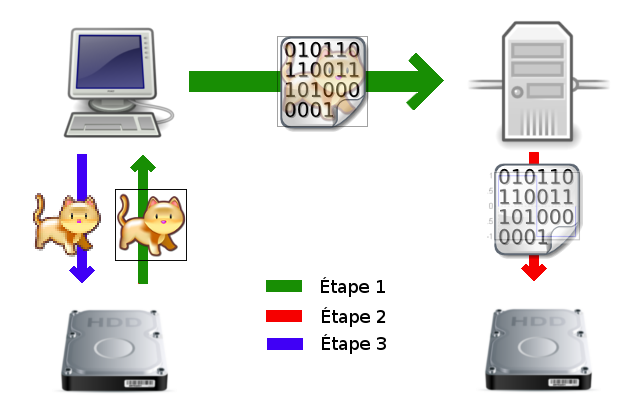
\includegraphics[scale=0.5]{images/save.png}
\caption{Processus d'archivage}
\label{save}
\end{figure}


\subsubsection{Processus de restauration}

\paragraph{Étape 1}

Le client crée une image à partir de celle qui avait été stockée en doublant ses dimensions, ainsi, chaque pixel devient un carré de 4 pixels.

\paragraph{Étape 2}

Le client demande les coefficients d'ondelette au serveur en spécifiant le nom de l'image. Le serveur lit le fichier qui contient les coefficients qu'il avait enregistrés et envoie directement les données au client.

\paragraph{Étape 3}

Le client décode les données binaires reçues et opère la transformation inverse en remplaçant les pixels de chaque carré par les valeurs qu'il obtient. Ensuite, il peut afficher l'image ou la stocker.\\

La figure \ref{load} illustre ce processus

 
\begin{figure}[!h]
\centering
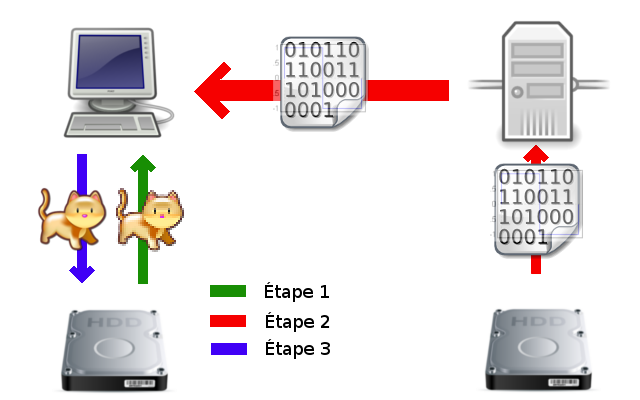
\includegraphics[scale=0.5]{images/load.png}
\caption{Processus de restauration}
\label{load}
\end{figure}


\clearpage

\section{Description du code}

Ce qui suit est une description du code de tous nos programmes.

\subsection{Le fichier ondelettes.py }

Dans ce fichier, nous définissons des classes qui permettent le traitement des images. Il peut très bien être utilisé tout seul (sans l'interface graphique). 

\subsubsection{La classe Matrice }

Au lieu d'utiliser la classe Matrice du module @numpy@, nous avons préféré créer la notre. En effet, nous n'avons pas besoin de toutes les fonctions qu'elle offre. Aussi, nous voulions faire un maximum de choses nous-mêmes.

\paragraph{La fonction init }

Cette fonction prend en argument la taille de la matrice et le premier élément qu'elle doit contenir pour ensuite créer un tableau de tableaux contenant ce premier élément. Elle enregistre aussi les dimensions de la matrice dans l'objet créé.

\paragraph{La fonction transpose }

Comme son nom l'indique, elle transforme la matrice en sa transposée. Elle est utilisée lors de la transformation par ondelettes de Haar.

\paragraph{La fonction add}

Elle permet l'addition de matrices. La matrice sur laquelle est appelée la fonction est replacée par le résultat de l'addition. Elle n'est pas utilisée dans ce programme, mais pour que notre classe soit réutilisable dans d'autres projets, il fallait qu'elle soit créée.

\paragraph{La fonction multiply}

Cette fonction est analogue à la fonction @add@ pour la multiplication.

\paragraph{La fonction copy}

Cette fonction transorme la matrice en celle qui est passée en argument.

\paragraph{La fonction update}

Cette fonction met à jour les dimensions de la matrice si le tableau a changé de taille.

\paragraph{Les fonctions save et save1} 

Elles permettent de sauvegarder l'état de la matrice dans un tableau auxilliaire.

\paragraph{La fonction restore}

Elle remet en place le tableau sauvegardé par la fonction @save@.


\subsubsection{La classe MatriceImage}

Cette classe utilise la classe @Matrice@ pour stocker une image afin de pouvoir travailler dessus. Elle contient également des fonctions de compression et d'enregistrement.

\paragraph{La fonction init}

Cette fonction prend en argument l'emplacement d'une image et la charge à l'aide de PIL. Elle crée puis remplit une @Matrice@ avec les informations des pixels de l'image (cf. fonction @fill@).

\paragraph{La fonction fill}

Cette fonction stocke les pixels de l'image dans la @Matrice@.

\paragraph{Les fonctions grayscalemean et grayscalemeanmatrix}

Elles transforment l'image en nuances de gris en remplaçant chaque couleur de chaque pixel par la moyenne des trois composantes RGB du pixel.
@grayscalemean@ fait l'opération sur l'image directement alors que @grayscalemeanmatrix@ la fait sur la @Matrice@ de l'image.

\paragraph{Les fonctions getmatrixred, getmatrixgreen et getmatrixblue}

Créent des tableaux dans l'objet et les remplissent avec les composantes RGB (respectivement) de l'image. Cela permet de traiter chaque couleur séparément.

\paragraph{La fonction save}

Elle prend en argument une chaîne de caractère et sauvegarde l'image sous ce nom dans le dossier courant.

\paragraph{La fonction ondelette\_{}haar}

Cette fonction prend en argument un tableau de valeurs et le nombre de récursions qu'elle doit faire. Elle renvoie le tableau des coefficients d'approximation ainsi que le tableau des coefficients d'ondelette.

\paragraph{Les fonctions getcolonne et getligne}

Ces fonctions servent à récupérer une liste contenant les données d'une colonne/d'une ligne, pour pouvoir ensuite être traitées par la fonction ondelette\_{}haar.


\paragraph{La fonction setcolonne}

Elle permet de remettre une colonne dans une matrice après traitement.

\paragraph{Les fonctions apply\_{}haar\_{}lig et apply\_{}haar\_{}col}

Ces fonctions appliquent la transformation avec l'ondelette de haar à toutes les lignes/toutes les colonnes d'une matrice.

\paragraph{La fonction haar\_{}grayscale}

Cette fonction convertit une image en nuances de gris, puis applique la transformation par ondelettes sur l'image. Elle l'applique d'abord sur les lignes, puis transpose la @Matrice@, puis la réapplique sur les lignes.

\paragraph{La fonction update}

Elle est similaire à celle qui a été décrite plus haut.

\paragraph{La fonction create\_{}coef\_{}matrix}

Elle crée les tableaux nécessaires à la mise en mémoire des coefficients d'ondelette de chaque couleur.

\paragraph{La fonction haar}

Elle a le même effet que la fonction @haar\_{}grayscale@, mais elle s'applique aux 3 composantes de l'image.

\paragraph{La fonction makeimage}

Cette fonction crée une image à partir des matrices des coefficients d'approximation.

\paragraph{La fonction compression}

Cette fonction, une fois que les matrices de coefficients d'ondelette ont été créées, permet de supprimer les coefficients qui sont inférieurs au @epsilon@ passé en paramètre.

\paragraph{Les fonctions syntheseligne et synthesecolonnes}

Ces fonctions appliquent la transformation inverse à l'image, à partir des coefficients d'approximation et des coefficients d'ondelette qui ont été conservés par la fonction @compression@.

\paragraph{La fonction clearimage}

Elle supprime toutes les données d'une image en la remplissant d'une couleur définie.

\paragraph{La fonction fasthaar}

Cette fonction permet d'appliquer la transformation par ondelettes sans passer par les matrices. Pour cela elle prend tous les <<carrés>> de 4 pixels d'une image et leur applique la transformation et la compression. Elle est plus rapide que les autres fonctions, mais l'inconvénient est que la récursivité n'est pas permise. Elle est donc utilisée pour compresser légèrement une image. Les résulats restent tout de même impressionnants puisqu'elle peut faire gagner jusqu'à 45\% d'espace en seulement quelques secondes.


\subsection{Le fichier ondelettesGUI.py}

Ce fichier est l'interface graphique du programme, qui requiert le fichier @ondelettes.py@ pour fonctionner. En effet, l'interface graphique n'est qu'une façade pour les fonctions qui ont été décrites plus haut.

\subsubsection{La classe Appli}

Cette classe représente la fenêtre principale de l'application.

\paragraph{La fonction init}

Cette fonction définit simplement l'instance de la fenêtre en appelant la fonction @initUI@ décrite plus bas.

\paragraph{La fonction initUI}

Cette fonction crée tous les éléments de la fenêtre (le titre et les menus, entre autres).

\paragraph{La fonction askopenfilename}

Cette fonction ouvre une boîte de dialogue demandant quel fichier ouvrir. La boite de dialogue est incluse dans l'installation de Tkinter.
Une fois que le fichier a été choisi, la fonction crée la zone où l'image sera affichée.

\paragraph{La fonction asksaveasfilename}

Cette fonction ouvre une boîte de dialogue demandant où enregistrer le fichier qui a été modifié.

\paragraph{Les fonctions askcompression et askcompression2}

Elles servent à ouvrir une boîte de dialogue du type @DialogScale@ (défini plus bas) pour demander à l'utilisateur le seuil de compression à utiliser lors de l'appel des fonctions @compression@ ou @compression2@.

\paragraph{Les fonctions compression et compression2}

Ces fonctions utilisent respectivement les fonctions @haar@ et @fasthaar@ de @ondelettes.py@ pour réaliser la compression de l'image avec le seuil donné par les fonctions @askcompression@ et @askcompression2@. L'ancienne image est ensuite effacée de l'écran et la nouvelle est affichée grâce à @displayimage@;

\paragraph{La fonction grayscale}

Elle utilise les fonctions de @ondelettes.py@ pour convertir l'image en nuances de gris.

\paragraph{La fonction displayimage}

Elle crée une zone pour afficher la nouvelle image qui a été créée par compression, puis l'affiche dans cette zone.

\paragraph{La fonction onExit}

Elle est appelée lors de la fermeture de l'application et est là pour être sûr que tout est fermé correctement.


\subsubsection{La classe DialogScale}

C'est la classe qui définit la boîte de dialogue de compression (Fig.\ref{GUI2}). Elle est construite sur la même base de fenêtre que la classe @Appli@.

\paragraph{La fonction initUI}

Cette fonction crée le texte de la boîte de dialogue, la réglette qui permet de choisir la compression, et le bouton <<Ok>>.

\paragraph{La fonction onScale}

Elle est appelée lorsque l'utilisateur modifie la position de la réglette. Elle stocke la position de celle-ci en mémoire. 

\paragraph{La fonction ok}

Elle est appelée lorsque l'utilisateur clique sur le bouton <<ok>>. Elle sauvegarde la valeur de la position de la réglette, puis ferme la boîte de dialogue.

\subsubsection{La fonction main}

Elle crée simplement une instance de la classe @Appli@ et l'exécute.


\subsection{Le fichier bench.py}

Ce fichier a été utilisé pour le chronométrage de l'algorithme @fasthaar@, expliqué plus haut.

\subsubsection{La fonction image\_gen}

Cette fonction crée une instance d'une image PIL dont la taille est passée en paramètre.

\subsubsection{La fonction randomize}

Elle prend en paramètre une image créée par @image_gen@, pour la remplir de pixels aléatoires. Afin d'être sûr que l'algorithme @fasthaar@ fera des calculs.

\subsubsection{La fonction bench\_square}

Cette fonction prend en argument un tableau de nombres qui vont servir à créer des images de tailles différentes avec @image_gen@, puis les remplir avec @randomize@ et enfin chronométrer le traitement de celles-ci avec le module @time@ de Python.

\subsubsection{La fonction fasthaar}

C'est la même que celle du fichier @ondelettes.py@ sauf qu'elle n'a pas besoin de la classe @ImageMatrice@ pour fonctionner.

\subsubsection{La fonction main}

Elle appelle la fonction @bench_square@ sur un tableau de nombres allant de 1 à 1000 (pour des images de 2 à 2000 pixels de côté).



\subsection{Le fichier serveur.py}


Ce fichier est celui qui est exécuté en permanence sur le serveur, comme décrit à la page \pageref{net}.

\subsubsection{La fonction main}

C'est la fonction principale du programme qui contient la boucle d'exécution du serveur. Elle commence par créer un @socket@ qui va attendre un client sur le port @13337@.

Lors de la connexion d'un client, le serveur entre dans la boucle d'exécution, qui tourne jusqu'à ce que le client envoie "stop" au serveur. À chaque fois que le client envoie un message au serveur, ce dernier en analyse les premières lettres pour connaître la commande que le client veut exécuter, puis l'exécute.

\subsubsection{La fonction recvImage}

Cette fonction est exécutée quand le client envoie "sendimg" au serveur. Le serveur récupère les dimensions de l'image, puis se met en attente des pixels de l'image, qu'il réceptionne dans une chaîne de caractères qui fait office de buffer. La réception se termine quand le client envoie "end". Le serveur décode ensuite la chaîne de caractère pixel par pixel en la parcourant par morceaux de 3 bytes, et insère les pixels décodés dans une image aux dimensions égales à celles qui ont été envoyées. Enfin, il enregistre l'image et signale au client que l'opération s'est complétée avec succès.

\subsubsection{La fonction fasthaar\_srv}

C'est une fonction qui ressemble à @fasthaar@ du fichier @ondelettes.py@, mais elle ouvre elle même un image à partir du nom envoyé par le client. Ensuite elle opère la transformation par ondelettes discrète et sauvegarde ceux-ci après les avoir encodés en binaire, uniquement s'ils sont supérieurs au paramètre optionnel epsilon (fixé à 0 par défaut, pour garder des images entières). Une fois que la transformation est terminée, le serveur le signale au client.

\subsubsection{La fonction sendCoef}

Cette fonction est appelée quand le client veut reconstituer une image. Il envoie alors @'coef nom_image'@. Le serveur ouvre le fichier qui contient les coefficients d'ondelette, et les envoie au client sans les décoder. Une fois que c'est terminé, le client envoie @"ok"@ en binaire au serveur pour lui signaler que l'opération s'est bien déroulée.

\subsection{Le fichier client.py}

Ce fichier est exécuté par le l'utilisateur quand il veut demander quelque chose au serveur (soit demander le stockage d'une image, soit demander des coefficients). Celui-ci est appelé de cette façon : \\ @./client.py [arguments:-rsd] image.jpg [optionnel : serveur]@

\subsubsection{La fonction main}

Cette fonction a pour arguments ceux passés par l'utilisateur en ligne de commande. Ils peuvent être :

\begin{itemize}
\item @r@ pour communiquer avec un serveur distant. Ce paramètre peut être omis pour établir la connection à un serveur local.

\item @s@ pour stocker une image. C'est à dire : envoi de l'image au serveur, compression de l'image par le serveur, enregistrement de l'image réduite par le client.

\item @d@ pour récupérer les coefficients d'ondelette d'une image et la reconstituer.

\end{itemize}


Dans le cas de l'utilisation de la commande @r@, on peut utiliser un serveur autre que celui définit par défaut en en spécifiant l'adresse après le nom de l'image à traiter. Une fois que l'échange client/serveur est terminé, la fonction envoie @"stop"@ au serveur, lui signifiant la fin de la connexion.

\subsubsection{La fonction sendImage}

Cette fonction est appelée lors de l'utilisation de la commande @s@, elle envoie au serveur @"sendimg"@ suivi des dimensions du nom de l'image et de ses dimensions. Ensuite l'image est encodée en binaire puis envoyée au serveur. Le client signale ensuite que le transfert est terminé en envoyant @"end"@ au serveur. Le client affiche ensuite la réponse du serveur.

\subsubsection{La fonction askcompress}

C'est la deuxième fonction appelée quand la commande @s@ est utilisée. Elle demande au serveur de compresser l'image qui a été envoyée plus tôt, avec @"compress"@ suivi du nom de l'image. Le client affiche ensuite la réponse du serveur.

\subsubsection{La fonction storeImage}

C'est la dernière fonction appelée quand la commande @s@ est utilisée. Cette fonction crée une image dont les dimensions ont été divisées par deux (par rapport à l'image originale) et y copie les coefficients d'approximation. Cette image est très légère et peut être affichée.

\subsubsection{La fonction askcoeff}

Cette fonction est appelée lors de l'utilisation de la commande @d@. Elle demande au serveur d'envoyer les coefficients d'ondelette de l'image. La fonction décode ensuite les coefficients reçus, puis ouvre l'image réduite qui avait été enregistrée par storeImage. Le client crée une image de la taille de l'image originale, puis opère la transformation par ondelettes inverse. Après ça, le client enregistre l'image.


\section{Conclusion}


La théorie des ondelettes symbolise en quelque sorte l'évolution des sciences mathématiques induite par l'introduction de l'outil informatique.
 
Bien que l'analyse par les ondelettes soit encore loin de nous donner une réponse universelle et finale au problème de la représentation et du codage des signaux, elle se révèle être un outil mathématique particulièrement performant dans plusieurs domaines, comme l'aura très nettement montré notre implémentation informatique.
D'ailleurs, nous aurons nous-mêmes pu exploiter la richesse des ondelettes dans le domaine de transferts-échanges de fichiers en proposant un service qui permet la compression d'images et leur affichage grâce à la connexion à un ordinateur distant.



\section{Bibliographie, Liens et Remerciements}
\label{links}
\begin{itemize}
\item http://www.cmi.univ-mrs.fr/\textasciitilde{}melot/Master2/TPsignal\_PS.html

\item Tous les fichiers .tex, .py de ce document :

https://github.com/timosis/TIPE2013-2014

\item L'interpréteur Python : http://www.python.org/

\item La librairie PIL pour Python : http://www.pythonware.com/products/pil/

\item La licence Creative Commons BY-SA :

http://creativecommons.org/licenses/by-sa/3.0/

\item Remerciements à : M. Petitjean
\end{itemize}


\clearpage
\lstset{language=Python,frame=single,breaklines=true,extendedchars=true, numbers=left,basicstyle=\footnotesize}
\section{Annexes}

Tout le code de ce projet est sous licence Creatice Commons BY-SA (voir p.\pageref{links}).


\subsection{Fichier ondelettes.py}
\lstinputlisting{ondelettes.py}

\subsection{Fichier ondelettesGUI.py}
\lstinputlisting{ondelettesGUI.py}

\subsection{Fichier bench.py}
\lstinputlisting{bench.py}

\subsection{Fichier serveur.py}
\lstinputlisting{serveur.py}

\subsection{Fichier client.py}
\lstinputlisting{client.py}

\begin{center}

\includegraphics{images/88x31.png}

\end{center}


\end{document}

